%%% Local Variables:
%%% mode: latex
%%% TeX-master: t
%%% End:

\documentclass[master, secret]{thuthesis}

\usepackage{thutils}
\usepackage{tabu}

%% Settings for add uppaal code 
\usepackage{pstricks}
\usepackage{latexsym,multicol,color}
\usepackage{listings} % comes with texlive−latex−recomended

\lstdefinelanguage{Uppaal}{ % syntax highlight via font
	basicstyle=\small\sffamily, % small sans−serif font (like verdana)
	keywords={after update,assign,before update,break,case,const,continue,
		default,else,enum,for,guard,if,meta,process,progress,return,select,
		state,sync,switch,trans,system,while},
	keywords={[2]broadcast,bool,clock,chan,commit,init,int,scalar,struct,
		typedef,urgent,void}, keywordstyle={[2]\bfseries},
	keywords={[3]false,true}, otherkeywords={[3]−>},
	morekeywords={[3]−>}, keywordstyle={[3]\bfseries},
	comment=[l]{//}, morecomment=[s]{/∗}{∗/}, % single and multi−line
	commentstyle=\itshape, % appear in italic
	tabsize=4, % tab treatment (going to be fixed in Uppaal)
	captionpos=b, % put captions at the bottom
	escapechar=@ % write LaTeX comments escaped by @ symbol
}
\lstdefinelanguage[GUI]{Uppaal}[]{Uppaal}{ % syntax like in GUI
	keywordstyle={[2]\color{black!50!green}}, % slightly darker than in GUI
	otherkeywords={−>}, keywordstyle={[3]\color{magenta}},
	commentstyle={\color{black!50!red}\itshape}, % dark red
	literate={{−−>}{$−−>$}3} % fix arrows
}
\lstdefinelanguage[LIT]{Uppaal}[GUI]{Uppaal}{ % replace some symbols
	literate={{−>}{{$\leadsto$} }2 {−−>}{{$\longrightarrow$} }2
		{=}{{$\gets$ }}2 {==}{{$==$}}2 {:=}{{$\gets$ }}2 {<=}{{$\leq$ }}2
		{>=}{{$\geq$ }}2 {&&}{{$\land$}}2 {||}{{$\lor$}}2 {<>}{{$\Diamond$}}1
		{[]}{{$\Box$}}1 {forall}{{$\forall$}}1 {exists}{{$\exists$}}1}
}
\lstset{language={[GUI]Uppaal}, % use GUI flavor
	columns={[l]flexible},
	frame=single, rulesepcolor=\color{gray},
	numbers=left,xleftmargin=4em,xrightmargin=4em, aboveskip=1em}
%% End of Setting

\usepackage[shortlabels]{enumitem}
\setlist[description]{style=multiline, leftmargin=7em, labelindent=\parindent}

%% to make use of property
\usepackage[amsmath,thmmarks]{ntheorem}
\newtheorem{property}{性质}[chapter]

\def\mycommand{\bgroup\obeyspaces\mycommandaux}
\def\mycommandaux#1{\mycommandauxii #1\relax\relax\egroup}
\def\mycommandauxii#1{%
	\ifx\relax#1\else \ifcat#1\@sptoken{} \expandafter\expandafter\expandafter\mycommandauxii\else
	\ifnum`#1=\uccode`#1 {\normalsize #1}\else {\footnotesize \uppercase{#1}}\fi \expandafter\expandafter\expandafter\mycommandauxii\expandafter\fi\fi}
\def\uppaal {\mycommand{Uppaal}}

% 你可以在这里修改配置文件中的定义,导言区可以使用中文。
\def\myname{刘盛鹏}
\def\intel{Intel\textsuperscript{\textregistered}}
\def\fpri{get\_highest\_pir}

\begin{document}
	
% 定义所有的eps文件在 figures 子目录下
\graphicspath{{figure/}}


%%% 封面部分
\frontmatter

\ctitle{基于时间自动机的\\中断实时性分析与验证}
% 根据自己的情况选,不用这样复杂
\makeatletter
\ifthu@bachelor\relax\else
  \ifthu@doctor
    \cdegree{工学博士}
  \else
    \ifthu@master
      \cdegree{工学硕士}
    \fi
  \fi
\fi
\makeatother


\cdepartment[软件学院]{软件学院}
\cmajor{软件工程}
\cauthor{刘盛鹏} 
\csupervisor{顾明教授}
% 如果没有副指导老师或者联合指导老师,把下面两行相应的删除即可。
%\cassosupervisor{贺飞教授}
% 日期自动生成,如果你要自己写就改这个cdate
%\cdate{\CJKdigits{\the\year}年\CJKnumber{\the\month}月}

% 博士后部分
% \cfirstdiscipline{计算机科学与技术}
% \cseconddiscipline{系统结构}
% \postdoctordate{2009年7月——2011年7月}

\etitle{Timing Analysis on Interrupt\\Based on Timed Automata} 
% 这块比较复杂,需要分情况讨论:
% 1. 学术型硕士
%    \edegree:必须为Master of Arts或Master of Science(注意大小写)
%              “哲学、文学、历史学、法学、教育学、艺术学门类,公共管理学科
%               填写Master of Arts,其它填写Master of Science”
%    \emajor:“获得一级学科授权的学科填写一级学科名称,其它填写二级学科名称”
% 2. 专业型硕士
%    \edegree:“填写专业学位英文名称全称”
%    \emajor:“工程硕士填写工程领域,其它专业学位不填写此项”
% 3. 学术型博士
%    \edegree:Doctor of Philosophy(注意大小写)
%    \emajor:“获得一级学科授权的学科填写一级学科名称,其它填写二级学科名称”
% 4. 专业型博士
%    \edegree:“填写专业学位英文名称全称”
%    \emajor:不填写此项
\edegree{Master of Engineering} 
\emajor{Software Engineering} 
\eauthor{Liu Shengpeng} 
\esupervisor{Professor Gu Min} 
%\eassosupervisor{Professor He Fei} 
% 这个日期也会自动生成,你要改么?
% \edate{December, 2005}

% 定义中英文摘要和关键字
\begin{cabstract}
   本文总结了三种常见的中断类型,分析了他们的软硬件实现。从实时性角度,本文对这
   些中断构造了相应的时间自动机模型。结合实际项目,本文应用该建模方法对某嵌入式
   平台上的中断驱动程序中的中断在\uppaal 中进行建模,并分析和验证了其实时性性质,
   对其中违反实时性约束的中断设置给出了反例。
\end{cabstract}

\ckeywords{中断,时间自动机,实时性,建模,验证}

\begin{eabstract} 
   The thesis summerized three most common types of interrupts and analyzed
   their implementation from the perspectives of both hardware and software.
   Focusing on the timing property, this thesis constructed models of the 
   timed automata of the thses interrupts .It gives all the specifics on 
   abstraction and modelling. The thesis applied the same approach on a set 
   of interrupt-driven software on some embedded platform from an actual 
   project. After analysis and verification on its timing properties, the 
   thesis proved there was a flaw in the interrupt setting and produced a 
   counter example.
\end{eabstract}

\ekeywords{Interrupt, Timed Automata, Timing, Model, Verification}

\makecover

% 目录
\tableofcontents

% 符号对照表
% \begin{denotation}

\item[HPC] 高性能计算 (High Performance Computing)
\item[cluster] 集群
\item[Itanium] 安腾
\item[SMP] 对称多处理
\item[API] 应用程序编程接口
\item[PI]	聚酰亚胺
\item[MPI]	聚酰亚胺模型化合物,N-苯基邻苯酰亚胺
\item[PBI]	聚苯并咪唑
\item[MPBI]	聚苯并咪唑模型化合物,N-苯基苯并咪唑
\item[PY]	聚吡咙
\item[PMDA-BDA]	均苯四酸二酐与联苯四胺合成的聚吡咙薄膜
\item[$\Delta G$]  	活化自由能~(Activation Free Energy)
\item [$\chi$] 传输系数~(Transmission Coefficient)
\item[$E$] 能量
\item[$m$] 质量
\item[$c$] 光速
\item[$P$] 概率
\item[$T$] 时间
\item[$v$] 速度
\item[劝  学] 君子曰:学不可以已。青,取之于蓝,而青于蓝;冰,水为之,而寒于水。
  木直中绳。(车柔)以为轮,其曲中规。虽有槁暴,不复挺者,(车柔)使之然也。故木
  受绳则直, 金就砺则利,君子博学而日参省乎己,则知明而行无过矣。吾尝终日而思
  矣,  不如须臾之所学也;吾尝(足齐)而望矣,不如登高之博见也。登高而招,臂非加
  长也,  而见者远;  顺风而呼,  声非加疾也,而闻者彰。假舆马者,非利足也,而致
  千里;假舟楫者,非能水也,而绝江河,  君子生非异也,善假于物也。积土成山,风雨
  兴焉;积水成渊,蛟龙生焉;积善成德,而神明自得,圣心备焉。故不积跬步,无以至千
  里;不积小流,无以成江海。骐骥一跃,不能十步;驽马十驾,功在不舍。锲而舍之,朽
  木不折;  锲而不舍,金石可镂。蚓无爪牙之利,筋骨之强,上食埃土,下饮黄泉,用心
  一也。蟹六跪而二螯,非蛇鳝之穴无可寄托者,用心躁也。\pozhehao{} 荀况
\end{denotation}



%%% 正文部分
\mainmatter
%%% Local Variables:
%%% mode: latex
%%% TeX-master: t
%%% End:

\chapter{引言}
\label{cha:intro}
%引出问题。

\section{中断}
\label{sec:intr}
中断(Interrupt)是指处理器接收到特殊信号,提示某个事件发生,应当采取
对应措施的情况。发出这样的信号的行为被称作中断请求(Interrupt Request,
IRQ)。这个信号可以是来自外围硬件的异步信号,也可以是由运行在处理器上的
软件发出同步信号。前者被称为硬件中断(Hardware Interrupt),后者则被
称为软件中断(Software Interrupt,常简称为软中断)。

处理器在接收到中断信号以后,通常会保存当前的执行状态,该执行状态被称为上
下文(Context)。上下文的内容视各个硬件平台的不同而有所区别,但是大多包
含程序计数器和程序状态字以及部分通用计算寄存器。之后,处理器会根据中断向
量表的指示跳转到指定代码片段,即当前中断的处理程序。在执行完中断处理程序
之后,处理器会重新加载之前保存的上下文,继续执行之前被打断的程序。进入中
断和退出中断都包含了将保存当前上下文,载入新的上下文的操作。此类操作被称
作为上下文切换(Context Switch)。\footnote{严格意义上的上下文切换
并不要求保存一个完好的上下文,载入另一个完好的上下文,实际情况中经常发生
载入的上下文只有部分内容有意义的情况。或者对原有上下文并未做出妥善保存即
另行载入,相当于舍弃了当前上下文。这在处理器响应中断时尤其多见。}

人们引入中断是为了提高计算机系统的性能。如果没有中断,处理器在接受外部硬
件通信时只能采取轮询方式。例如,处理器向某硬件发出某指令并需求其回复时,
只能采取繁忙等待(Busy-waiting)模式,这样就会浪费许多处理器周期。即使
在软件层面运用多线程技术进行优化,此类轮询操作依然是性能的损失。在引入中
断之后,处理器就可以专注于当前任务,并且可以在需要时候与外部硬件通信,从
而大幅提高运行效率。\footnote{处理器检查中断的原理其实也类似于一个轮询
操作。每个周期,处理器会检查特定的寄存器的某些位来判断是否有中断需要处理。
只不过这个处理相比于外部硬件通信快速得多。}后来被用于CPU外部与内部紧急事
件的处理、机器故障的处理、时间控制等多个方面,并产生通过软件方式进入中断
处理(软中断)的概念。在处理中断时几乎必然会触发两次切换上下文的操作,该
操作会涉及内存访问,因此其耗时在中断处理程序本身比较短的时候也不可忽略。
过于频繁的中断触发也会在一定程度降低系统的性能。

中断系统在硬件实现上可以是一个包含控制线路的独立系统,也可以被集成进存储
器子系统中。对于前者,在IBM个人机上,广泛使用可编程中断控制器(Programmable 
Interrupt Controller,PIC)来负责中断响应和处理。PIC被连接在若干中
断请求设备和处理器的中断引脚之间,从而实现对处理器中断请求线路(多为一针
或两针)的复用。作为另一种中断实现的形式,即存储器子系统实现方式,可以将
中断端口映射到存储器的地址空间,这样对特定存储器地址的访问实际上是中断请
求。一般桌面领域的PC机中,中断控制器一般是集成在处理器内部,\footnote{
例如\intel{}推出的8086系列处理器中,集成了\intel{} 8259系列中断控制器。}
而在嵌入式领域,很多厂商推出的微控制器实现了外置的中断控制器。\footnote{
例如意法半导体(STMicroelectronics)推出的STM32F4系列微控制器中,在ARM
的CPU外提供了中断控制器。}

\subsection{操作系统中的中断}
\label{subsec:intr_OS}
在实际应用中,中断的行为并不一直忠实地遵从其硬件实现,操作系统可以在一定
程度上改变中断的行为。在嵌入式操作系统中,出于实时性的考虑,一个中断的运
行时间不应该过长,但是许多中断需要实现的逻辑功能却比较复杂。因此一个通用
的解决方案就是在操作系统中将中断分成两段,前一段在中断触发时立即执行,后
一段则延后执行。后一段代码的执行优先级较低,因此有可能被其他低优先级中断
甚至是普通代码抢先执行。这样,在编写中断代码的时候,将需要立即执行不容延
迟同时运行时间较短的代码放在第一段,其他的对延时不敏感,或者任务繁重,或
者需要和其他线程进行同步交互的代码放在第二段,就能在满足实时性要求的前提
下完成该中断。eCos等许多操作系统尽管实现方式各异,采用的都是分段中断的模
式。\cite{ecos}图~\ref{fig:intr_exec} 和图~\ref{fig:ecos_intr_exec} 
分别展示了两种中断的执行流。

\begin{figure}[H]
	\centering
	\subcaptionbox{普通中断的执行流\label{fig:intr_exec}}
	{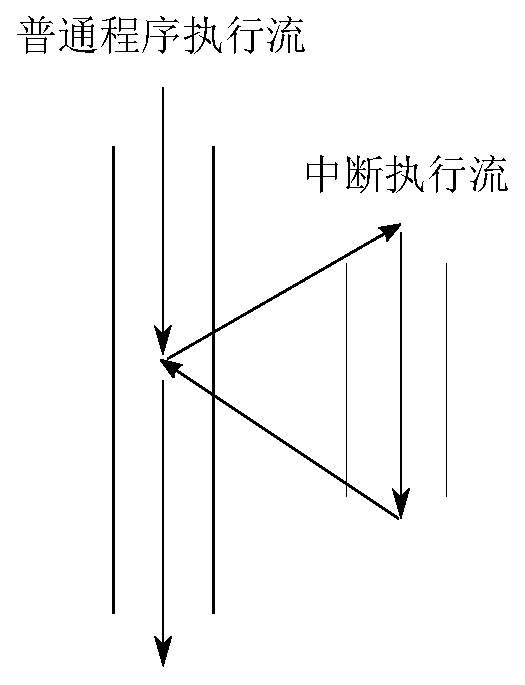
\includegraphics[width=0.35\textwidth]{interrupt_exec_model}}
	\hspace{4em}%
	\subcaptionbox{分段中断的执行流\label{fig:ecos_intr_exec}}
	{\includegraphics[width=0.35\textwidth]{ecos_interrupt_model}}
	\caption{不同的中断执行流}
	\label{fig:two_intr_exec}
\end{figure}

\section{程序的正确性}
\label{sec:correctness}
人们通常关心程序的许多性质。我们常说一个程序是否正确,其实涵盖了很多方面。

程序正确性,从狭义上来说,是指一段代码实现的功能是否如预期。这个要求并没
有看上去那么简单。程序不仅在接受各种合法输入之后需要给出预期的输出,在接
受非法输入之后也应该能判断出输入非法,并作出相应的处理措施。

从广义上来说,程序正确性还包含了其在指定环境下运行的正确性。现在的程序很
少是完全孤立运行。大部分程序运行在操作系统中,需要与其他程序共享CPU,内
存,硬盘,网络等资源。那么,程序的正确性就包含了该程序在共享资源的条件下
依然能保持上述狭义的正确性质。对多线程程序的研究就是着眼于多个线程在共享
CPU的条件下能否保证其功能的正确,尤其是当线程间共享的资源不仅仅是CPU,
还有内存中的变量,共同的文件或网络链接等资源时,情况将变得更加复杂。即使
在单线程的运行环境中,程序还会受到中断的干扰\footnote{上述的多线程的环
境下,通常也是有中断存在的。多线程的时间片轮转模式就完全依赖时钟中断。只
不过由于多线程的运行环境已经十分复杂,许多研究就忽略了中断的参与以简化问
题。}除了时钟中断以外的其他中断相比多线程环境,行为的随机性更高,一旦出现
问题,想要完全重现问题场景更为困难,研究起来更加困难。

由于外部环境的参与,一些原本不属于正确性的性质也会对程序的正确运行产生影
响。举个例子,程序的运行时间在大多数情况,本与程序是否正确没有关系,从软
件工程的需求分析角度来说,运行时间,或者说效率只能算作程序的非功能需求。
一段程序运行时间长短似乎不会影响到程序运行的结果。然而,事实并非总是如此。

当程序的运行时间影响到共享资源的占用,而共享资源又对程序的功能正确性造成
影响的时候,程序的运行时间就会成为程序正确性的内涵之一。这在一些十分接近
硬件底层的程序中,体现得尤为明显。举个简单的例子,一个简单的Clinet-Server
(CS)架构,一个客户端和一个服务器。客户端给服务器发送一个请求,经过一段
时间服务器返回结果,客户端继续一段逻辑。在网络编程中,考虑到网络环境的不
稳定性,程序员通常会设置等待超时,即当一定时间后得不到网络另一端的响应,
就认为此次请求失效,接下来就进行例如重发等措施。在这个场景下,服务器接受
请求返回应答的程序的运行时间就会成为影响客户端程序正确性的因素。在极端情
况下,服务器端程序的运行时间过长,客户端一直无法在超时限制之前得到响应,
那么客户端的正常逻辑就永远无法进行下去。

在实时软件系统中,由于实时性要求非常高,大部分程序的运行时间都是其正确性
的关键内容。在大部分实时软件系统中,中断多且与整个软件系统的功能息息相关。
的正确性就显得尤为重要。中断本身的难以预测,中断之间的相互作用又
使得中断的时间性质验证相对困难。

\section{程序的验证技术}
\label{sec:verification}
编程技术发展至今,软件的验证技术已经日趋成熟。根据是否运行程序,我们可以
将验证技术分为动态验证技术和静态验证技术两大类。

\subsection{动态验证技术}
\label{subsec:dynamic}
动态验证即我们通常所谓的测试。根据测试范围的不同,我们可将测试分为三类。
\cite{SWEBOK}
\begin{itemize}
	\item 小范围测试:测试一个函数或一个类(单元测试)
	\item 大范围测试:测试一组类,例如
	\begin{enumerate}[(1)]
		\item 模块测试(测试一个模块)
		\item 集成测试(测试多个模块)
		\item 系统测试(测试整个系统)
	\end{enumerate}
	\item 验收测试:验证软件是否满足需求的正式测试
	\begin{enumerate}[(1)]
		\item 功能测试
		\item 非功能测试(性能测试,压力测试等)
	\end{enumerate}		
\end{itemize}
测试一直时软件工程中十分重要也是最常规的验证的手段。在大多数场合,软件测
试成本低,效果显著。在成熟的软件公司或软件开发团队中,都有专门从事测试的
部门或人员。

\subsection{静态验证技术}
\label{subsec:static}
静态验证指在不运行程序的前提下,对程序进行的验证。有些程序的测试成本太高,
或者测试用例无法覆盖正常运行时的很多情形,即当我们无法测试程序,或者测试
结果局限性太严重时,我们转向静态验证。静态验证的技术发展多年,已经有了很
多相对成熟的方案。例如:
\begin{itemize}
	\item 代码规范检查
	\item 反例检测
	\item 形式化验证
	\begin{enumerate}[(1)]
		\item 模型检测
		\item 定理证明
	\end{enumerate}	
\end{itemize}

在静态分析技术中,形式化验证利用形式化方法对程序性质进行验证,由于其在理
论上的可靠性受到学术界密切关注。常规的测试很难甚至不可能在可以容忍的时间
内覆盖所有的可能情况,但是形式化验证技术则在理论上有给出一个完全覆盖所有
可能的测试结果的可能。这就是形式化验证相比传统动态验证技术的最大优势。

%这一段加引用
在诸多形式化验证技术中,模型检测由于数学要求相对不高,自动化程度较高,工
具化较为容易,在学术界较为流行。定理证明作为另一个完全不同的分支,由于自
动化程度和工具化程度太低,大量工作需要人的手工参与,因此使用者相对较少,
应用数量较少。但是,这模型检测和定理证明在大规模项目上的应用都有限制。前
者受理论和计算机硬件的限制,状态空间爆炸这个问题一直无法根本解决。这也是
诸多学者一直在努力的方向之一。后者由于其理论依据中对高阶逻辑的支持,看似
可以在理论上解决空间爆炸的问题,但是由于目前定理证明主要还是靠人工参与推
理,面对大型项目,人工的推理几乎不可完成。理论上可以进行验证,但是成本过
于高昂,这也是工业界对形式化验证技术一直难以应用的主要原因。相比之下,传
统的测试技术,对项目敏感度没有形式化技术这么高,反而容易取得不错的结果。

然而,在一些领域,程序的正确性涉及到人身财产安全甚至国家安全,不完备的测
试几乎不可能满足正确性的验证要求。形式化验证看似很美好,但随着验证规模的
增长,成本也成指数级增长,这时一个折中的做法对验证对象进行一定的抽象,然
后再对抽象出的模型进行验证。通常,抽象之后的模型相比原程序在验证规模上会
缩小很多。如果能保证抽象过程对于待验证性质的保持,即针对待验证性质,程序
和抽象模型之间存在一个完好的精化关系,就可以对模型进行形式化验证。

\section{研究课题}
\label{sec:subject}
我的课题是基于Uppaal的中断时间性质分析和验证。课题来源于一个针对某嵌入
式平台的实时软件系统的验证项目。我希望利用时间自动机的理论分析中断的时间
性质,进而对某些性质给出肯定或否定的验证结论。

\subsection{Uppaal简介}
\label{subsec:Uppaal_intro}
%这一段加引用
UPPAAL是一个进行建模,仿真和验证实时系统的集成工具环境,由丹麦奥尔堡大
学的计算机科学基础研究中心(Basic Research in Computer Science, BRICS)和瑞典乌普萨拉大学信息技术系联合开发。它适合那些可以被建模为具有
有限的控制结构和实数值时钟,通过信道或共享变量通信的非确定性过程集合的系
统。典型的应用领域包括实时控制器和特定的实时性至关重要的通信协议。

\subsection{预期成果}
\label{subsec:expectation}
本课题预期有以下成果:
\begin{itemize}
	\item 在Uppaal中针对各类中断的时间自动机模型
	\item 针对某嵌入式平台的实时软件系统的中断的时间性质的验证
\end{itemize}

\section{论文结构}
\label{sec:structure}
本文第一章简要介绍我研究的课题以及相关背景。在第二章,本文将介绍一些有关
中断分析验证以及时间自动机的相关工作。在第三章,本文将描述对中断行为的分
析,中断模型的建立和利用时间自动机的分析过程。在第四章,本文将描述将本文
的理论模型应用某嵌入式平台的实施软件系统进行验证的实验过程以及实验结果。
在第五章,本文将对该课题工作进行总结。



%%% Local Variables:
%%% mode: latex
%%% TeX-master: t
%%% End:

\chapter{相关工作}
\label{cha:related_work}

%  × 时间自动机
%        秒表自动机(stopwatch automata) 
%		 CCS parallele composition
%  × 中断驱动程序验证
%  × 实时性分析

时间自动机是由Alur R.和D.L. Dill在上世纪九十年代出提出来的理论。他们用时间自动
机来描述实时系统在时间上的行为。他们从形式化语言的角度定义了时间自动机的语法和语
义\cite{Alur:1994:TTA:180782.180519}。该理论是对传统自动机理论\cite{Hopcroft:2006:IAT:1196416}
的一个重要扩展。得益于时间自动机的提出,自动机模型以及模型检测技术\cite{Clarke:2000:MC:332656}
才能将时间纳入系统的考虑。

在时间自动机理论中,时钟是一个连续的实数变量。同一个时间自动机系统里的时钟在每个
位置都均匀的增长。时钟的值在一些变迁中可以被重置为0,或者在某些变迁中用时钟的值
的范围作为条件。因此,时间自动机用来描述并发的依赖时间的行为是非常理想的。然而,
在某些情况下,例如抢占式调度,我们需要知道系统在某些位置停留的时间。时钟变量只能
被重置却不能被赋值。这就导致了对时间自动机的扩展。在这项扩展力,时钟在某些位置的
的导数可以是0,即意味着该时钟在该位置下停止计时。这样的自动机被称为聚合图(Integration
Graph)\cite{Kesten:1999:DIG:302392.302397}, 被作为时段演算(Duration Calculus)
\cite{DBLP:journals/ipl/ChaochenHR91}的模型进行研究。其研究成果包括此类自动机
的可达性问题的不可判定\cite{Alur04decisionproblems},以及在这类自动机的一个特
殊子类别上利用基于缩减问题到线性约束满足性问题\cite{Apt:2003:PCP:1237975}时有
一个可判定的过程。在混合自动机\cite{Henzinger96thetheory}的一项判定性研究
\cite{McManis:1994:SAD:647763.735660}中,提到了类似的自动机。同时,一项近似验
证算法的实现工作\cite{Cassez:2000:IPS:646735.701625}里也提到了该自动机。

该自动机由于其时钟暂停的特性有一个形象的名字\pozhehao 秒表自动机。除了上述的理
论性研究以外,还有人做了应用方面的探索\cite{Abdeddaim:2002:PJS:646486.694487}。

来自大阪大学的Makoto Higashi等人提出了一套在一个CPU模拟器上测试中断的方法以
检测中断带来的潜在数据竞争。该方法包含两个方面:第一是在可能产生数据竞争的指令处
触发中断,第二是人为修改外部中断给中断处理程序的输入。中断会在每次读或写内存的指
令之后触发,以此覆盖所有可能产生数据竞争的情况。外部中断的输入序列则是在程序运行
之前就手动准备好。他们已经在\emph{uClinux}上应用此方法做过实验。\cite{Higashi:2010:EMC:1808266.1808278}


%%% Local Variables:
%%% mode: latex
%%% TeX-master: t
%%% End:

\chapter{基于Uppaal的中断模型}
\label{cha:intr}

\section{Uppaal中的模型组成}
\label{sec:model_combine}	
一套Uppaal模型由以下三部分组成。
\begin{itemize}
	\item \emph{声明}:整个模型系统中共有的声明,可以是变量或函数。在整个
	系统中都可以访问。
	\item \emph{自动机模板}:各类自动机的通用模板,一个模型系统可以有多个
	模板,一个模板在系统中可以对应多个实例。
		\begin{enumerate}[(1)]
			\item \emph{声明}:模板内部的变量或函数,只有本模板的实例可
			以访问。
			\item \emph{位置}:时间自动机的位置,每个位置可以有初始(
			initial),紧急(urgent),关键(committed)。关键位置与紧
			急位置上,模型中的时钟都停止。不同的是,当有自动机在关键位置时,
			在下一个状态迁移必须从某一个关键位置发出。
			\item \emph{变迁}:位置到位置的迁移。变迁包含选择(select)
			、条件(guard)、同步(sync)、更新(update)四个属性。其中,
			同步和更新是同时发生的。
		\end{enumerate}	
	\item \emph{模型声明}:定义组成系统的模板实例。
\end{itemize}

\section{基本中断模型}
\label{sec:basic}
通常,在我们接触到的非实时性电脑环境中,中断的行为就是符合一个中断的基本模型。其
行为模式就是简单的抢占当前线程,在执行结束之后恢复上下文继续执行被抢占的线程。

\begin{figure}[H]
	\centering
	%LaTeX with PSTricks extensions
%%Creator: inkscape 0.91
%%Please note this file requires PSTricks extensions
\psset{xunit=.5pt,yunit=.5pt,runit=.5pt}
\begin{pspicture}(438.14290264,242.42857685)
{
\newrgbcolor{curcolor}{0 0 0}
\pscustom[linewidth=0.57914072,linecolor=curcolor]
{
\newpath
\moveto(300.71042076,199.7857195)
\curveto(300.71042076,223.17679387)(263.2000076,242.13900624)(216.92856804,242.13900624)
\curveto(170.65712849,242.13900624)(133.14671532,223.17679387)(133.14671532,199.7857195)
\curveto(133.14671532,176.39464514)(170.65712849,157.43243276)(216.92856804,157.43243276)
\curveto(263.2000076,157.43243276)(300.71042076,176.39464514)(300.71042076,199.7857195)
\closepath
}
}
{
\newrgbcolor{curcolor}{0 0 0}
\pscustom[linestyle=none,fillstyle=solid,fillcolor=curcolor]
{
\newpath
\moveto(217.19642083,184.4732195)
\curveto(216.46725416,183.2232195)(215.26933749,182.5982195)(213.60267083,182.5982195)
\lineto(210.32142083,182.5982195)
\curveto(208.23808749,182.5982195)(207.19642083,183.5357195)(207.19642083,185.4107195)
\lineto(207.19642083,204.4732195)
\lineto(205.16517083,204.4732195)
\curveto(205.26933749,198.74405283)(204.59225416,194.10863617)(203.13392083,190.5669695)
\curveto(201.77975416,187.1294695)(199.07142083,183.90030283)(195.00892083,180.8794695)
\lineto(194.54017083,181.3482195)
\curveto(197.76933749,184.1607195)(200.00892083,187.2857195)(201.25892083,190.7232195)
\curveto(202.61308749,194.26488617)(203.23808749,198.8482195)(203.13392083,204.4732195)
\lineto(201.41517083,204.4732195)
\lineto(200.00892083,204.1607195)
\lineto(198.75892083,205.4107195)
\lineto(203.13392083,205.4107195)
\curveto(203.13392083,212.18155283)(203.08183749,216.08780283)(202.97767083,217.1294695)
\lineto(206.25892083,215.5669695)
\lineto(205.16517083,214.4732195)
\lineto(205.16517083,205.4107195)
\lineto(212.50892083,205.4107195)
\lineto(214.38392083,207.2857195)
\lineto(217.04017083,204.4732195)
\lineto(209.22767083,204.4732195)
\lineto(209.22767083,186.1919695)
\curveto(209.22767083,184.9419695)(209.85267083,184.3169695)(211.10267083,184.3169695)
\lineto(212.35267083,184.3169695)
\curveto(213.49850416,184.3169695)(214.12350416,184.83780283)(214.22767083,185.8794695)
\curveto(214.33183749,187.02530283)(214.38392083,188.6919695)(214.38392083,190.8794695)
\lineto(215.16517083,190.8794695)
\lineto(215.47767083,187.1294695)
\curveto(215.68600416,185.8794695)(216.25892083,184.99405283)(217.19642083,184.4732195)
\closepath
\moveto(208.29017083,214.7857195)
\curveto(210.16517083,213.8482195)(211.46725416,213.01488617)(212.19642083,212.2857195)
\curveto(212.92558749,211.6607195)(213.18600416,210.93155283)(212.97767083,210.0982195)
\curveto(212.76933749,209.36905283)(212.40475416,208.79613617)(211.88392083,208.3794695)
\curveto(211.46725416,208.0669695)(211.05058749,208.58780283)(210.63392083,209.9419695)
\curveto(210.21725416,211.40030283)(209.33183749,212.85863617)(207.97767083,214.3169695)
\lineto(208.29017083,214.7857195)
\closepath
\moveto(186.88392083,204.4732195)
\lineto(186.88392083,198.8482195)
\lineto(195.47767083,198.8482195)
\lineto(195.47767083,204.4732195)
\lineto(186.88392083,204.4732195)
\closepath
\moveto(189.07142083,217.1294695)
\curveto(190.42558749,216.40030283)(191.46725416,215.67113617)(192.19642083,214.9419695)
\curveto(192.92558749,214.21280283)(193.18600416,213.5357195)(192.97767083,212.9107195)
\curveto(192.87350416,212.2857195)(192.56100416,211.71280283)(192.04017083,211.1919695)
\curveto(191.51933749,210.77530283)(191.05058749,211.24405283)(190.63392083,212.5982195)
\curveto(190.32142083,214.05655283)(189.64433749,215.46280283)(188.60267083,216.8169695)
\lineto(189.07142083,217.1294695)
\closepath
\moveto(181.72767083,210.4107195)
\lineto(196.72767083,210.4107195)
\lineto(198.44642083,212.1294695)
\lineto(201.10267083,209.4732195)
\lineto(186.88392083,209.4732195)
\curveto(185.32142083,209.4732195)(184.07142083,209.3169695)(183.13392083,209.0044695)
\lineto(181.72767083,210.4107195)
\closepath
\moveto(184.69642083,196.1919695)
\curveto(184.80058749,197.85863617)(184.85267083,199.57738617)(184.85267083,201.3482195)
\curveto(184.85267083,203.11905283)(184.80058749,204.88988617)(184.69642083,206.6607195)
\lineto(186.88392083,205.4107195)
\lineto(195.32142083,205.4107195)
\lineto(196.57142083,206.8169695)
\lineto(198.75892083,204.7857195)
\lineto(197.50892083,203.8482195)
\curveto(197.50892083,201.0357195)(197.56100416,198.79613617)(197.66517083,197.1294695)
\lineto(195.47767083,196.1919695)
\lineto(195.47767083,197.9107195)
\lineto(192.50892083,197.9107195)
\lineto(192.50892083,185.5669695)
\curveto(192.50892083,184.52530283)(192.24850416,183.74405283)(191.72767083,183.2232195)
\curveto(191.31100416,182.70238617)(190.58183749,182.23363617)(189.54017083,181.8169695)
\curveto(189.43600416,183.0669695)(188.08183749,184.10863617)(185.47767083,184.9419695)
\lineto(185.47767083,185.5669695)
\curveto(187.87350416,185.2544695)(189.33183749,185.0982195)(189.85267083,185.0982195)
\curveto(190.37350416,185.20238617)(190.63392083,185.5669695)(190.63392083,186.1919695)
\lineto(190.63392083,197.9107195)
\lineto(186.88392083,197.9107195)
\lineto(186.88392083,196.9732195)
\lineto(184.69642083,196.1919695)
\closepath
\moveto(188.75892083,193.0669695)
\lineto(187.35267083,192.2857195)
\curveto(185.26933749,189.05655283)(183.29017083,186.45238617)(181.41517083,184.4732195)
\lineto(180.94642083,184.7857195)
\curveto(182.09225416,186.55655283)(183.08183749,188.32738617)(183.91517083,190.0982195)
\curveto(184.85267083,191.86905283)(185.52975416,193.48363617)(185.94642083,194.9419695)
\lineto(188.75892083,193.0669695)
\closepath
\moveto(194.22767083,194.0044695)
\lineto(194.54017083,194.4732195)
\curveto(196.10267083,193.5357195)(197.19642083,192.7544695)(197.82142083,192.1294695)
\curveto(198.44642083,191.5044695)(198.75892083,190.82738617)(198.75892083,190.0982195)
\curveto(198.75892083,189.4732195)(198.44642083,188.79613617)(197.82142083,188.0669695)
\curveto(197.30058749,187.4419695)(196.88392083,187.85863617)(196.57142083,189.3169695)
\curveto(196.25892083,190.77530283)(195.47767083,192.33780283)(194.22767083,194.0044695)
\closepath
}
}
{
\newrgbcolor{curcolor}{0 0 0}
\pscustom[linestyle=none,fillstyle=solid,fillcolor=curcolor]
{
\newpath
\moveto(243.44642083,209.6294695)
\lineto(243.44642083,203.3794695)
\lineto(244.54017083,203.3794695)
\curveto(245.99850416,205.04613617)(247.56100416,207.1294695)(249.22767083,209.6294695)
\lineto(243.44642083,209.6294695)
\closepath
\moveto(240.16517083,196.0357195)
\lineto(240.16517083,191.3482195)
\lineto(250.47767083,191.3482195)
\lineto(250.47767083,196.0357195)
\lineto(240.16517083,196.0357195)
\closepath
\moveto(240.16517083,190.4107195)
\lineto(240.16517083,184.9419695)
\lineto(250.47767083,184.9419695)
\lineto(250.47767083,190.4107195)
\lineto(240.16517083,190.4107195)
\closepath
\moveto(237.97767083,180.8794695)
\curveto(238.08183749,183.48363617)(238.13392083,188.0669695)(238.13392083,194.6294695)
\curveto(235.21725416,192.54613617)(232.97767083,191.13988617)(231.41517083,190.4107195)
\lineto(231.10267083,190.8794695)
\curveto(234.01933749,192.96280283)(236.36308749,194.88988617)(238.13392083,196.6607195)
\curveto(238.13392083,197.18155283)(238.08183749,197.85863617)(237.97767083,198.6919695)
\lineto(239.22767083,197.7544695)
\curveto(240.89433749,199.3169695)(242.45683749,200.8794695)(243.91517083,202.4419695)
\lineto(237.97767083,202.4419695)
\curveto(236.62350416,202.4419695)(235.37350416,202.2857195)(234.22767083,201.9732195)
\lineto(232.82142083,203.3794695)
\lineto(241.41517083,203.3794695)
\lineto(241.41517083,209.6294695)
\lineto(239.85267083,209.6294695)
\curveto(238.49850416,209.6294695)(237.24850416,209.4732195)(236.10267083,209.1607195)
\lineto(234.69642083,210.5669695)
\lineto(241.41517083,210.5669695)
\curveto(241.41517083,214.0044695)(241.36308749,216.3482195)(241.25892083,217.5982195)
\lineto(244.69642083,216.0357195)
\lineto(243.44642083,214.9419695)
\lineto(243.44642083,210.5669695)
\lineto(245.16517083,210.5669695)
\lineto(247.19642083,212.2857195)
\lineto(249.38392083,210.0982195)
\curveto(250.21725416,211.3482195)(251.05058749,212.9107195)(251.88392083,214.7857195)
\lineto(254.85267083,212.5982195)
\curveto(254.01933749,212.38988617)(252.92558749,211.3482195)(251.57142083,209.4732195)
\curveto(250.32142083,207.5982195)(248.81100416,205.5669695)(247.04017083,203.3794695)
\lineto(252.19642083,203.3794695)
\lineto(254.38392083,205.4107195)
\lineto(257.04017083,202.4419695)
\lineto(246.41517083,202.4419695)
\curveto(244.64433749,200.5669695)(242.82142083,198.74405283)(240.94642083,196.9732195)
\lineto(250.16517083,196.9732195)
\lineto(251.25892083,198.5357195)
\lineto(253.75892083,196.5044695)
\lineto(252.50892083,195.5669695)
\lineto(252.50892083,185.5669695)
\curveto(252.50892083,184.21280283)(252.56100416,183.01488617)(252.66517083,181.9732195)
\lineto(250.47767083,181.0357195)
\lineto(250.47767083,184.0044695)
\lineto(240.16517083,184.0044695)
\lineto(240.16517083,181.8169695)
\lineto(237.97767083,180.8794695)
\closepath
\moveto(221.10267083,186.9732195)
\curveto(222.04017083,187.07738617)(223.65475416,187.33780283)(225.94642083,187.7544695)
\curveto(228.34225416,188.17113617)(231.36308749,188.74405283)(235.00892083,189.4732195)
\lineto(235.16517083,188.8482195)
\curveto(232.24850416,188.01488617)(229.69642083,187.23363617)(227.50892083,186.5044695)
\curveto(225.32142083,185.77530283)(223.70683749,184.9419695)(222.66517083,184.0044695)
\lineto(221.10267083,186.9732195)
\closepath
\moveto(228.44642083,217.1294695)
\lineto(231.57142083,215.2544695)
\curveto(230.73808749,214.83780283)(229.64433749,213.58780283)(228.29017083,211.5044695)
\curveto(226.93600416,209.52530283)(225.37350416,207.2857195)(223.60267083,204.7857195)
\lineto(230.79017083,204.9419695)
\curveto(231.62350416,206.29613617)(232.35267083,207.7544695)(232.97767083,209.3169695)
\lineto(235.47767083,207.2857195)
\curveto(234.33183749,206.45238617)(232.97767083,204.99405283)(231.41517083,202.9107195)
\curveto(229.95683749,200.82738617)(227.76933749,198.2232195)(224.85267083,195.0982195)
\curveto(227.76933749,195.51488617)(231.05058749,196.08780283)(234.69642083,196.8169695)
\lineto(234.85267083,196.1919695)
\curveto(232.14433749,195.35863617)(230.00892083,194.68155283)(228.44642083,194.1607195)
\curveto(226.88392083,193.63988617)(225.52975416,192.96280283)(224.38392083,192.1294695)
\lineto(222.35267083,195.4107195)
\curveto(223.18600416,195.7232195)(224.17558749,196.45238617)(225.32142083,197.5982195)
\curveto(226.46725416,198.74405283)(228.13392083,200.93155283)(230.32142083,204.1607195)
\curveto(228.44642083,203.95238617)(226.98808749,203.6919695)(225.94642083,203.3794695)
\curveto(224.90475416,203.17113617)(223.86308749,202.7544695)(222.82142083,202.1294695)
\lineto(221.10267083,204.9419695)
\curveto(222.04017083,205.04613617)(223.23808749,206.29613617)(224.69642083,208.6919695)
\curveto(226.15475416,211.08780283)(227.40475416,213.90030283)(228.44642083,217.1294695)
\closepath
}
}
{
\newrgbcolor{curcolor}{0 0 0}
\pscustom[linestyle=none,fillstyle=solid,fillcolor=curcolor]
{
\newpath
\moveto(61.52679148,62.75447382)
\lineto(75.12054148,62.75447382)
\lineto(77.30804148,64.78572382)
\lineto(80.12054148,61.81697382)
\lineto(65.74554148,61.81697382)
\curveto(65.01637481,61.81697382)(64.07887481,61.66072382)(62.93304148,61.34822382)
\lineto(61.52679148,62.75447382)
\closepath
\moveto(60.58929148,42.44197382)
\curveto(61.63095814,42.65030715)(62.62054148,43.32739048)(63.55804148,44.47322382)
\curveto(64.49554148,45.61905715)(65.48512481,47.07739048)(66.52679148,48.84822382)
\curveto(67.56845814,50.61905715)(68.29762481,52.23364048)(68.71429148,53.69197382)
\lineto(63.08929148,53.69197382)
\curveto(62.25595814,53.69197382)(61.26637481,53.53572382)(60.12054148,53.22322382)
\lineto(58.71429148,54.62947382)
\lineto(78.08929148,54.62947382)
\lineto(80.43304148,56.97322382)
\lineto(83.40179148,53.69197382)
\lineto(69.18304148,53.69197382)
\lineto(71.99554148,51.66072382)
\curveto(71.16220814,51.66072382)(69.91220814,50.51489048)(68.24554148,48.22322382)
\curveto(66.68304148,46.03572382)(64.96429148,44.00447382)(63.08929148,42.12947382)
\lineto(76.99554148,42.75447382)
\curveto(76.26637481,44.31697382)(75.12054148,45.98364048)(73.55804148,47.75447382)
\lineto(74.02679148,48.06697382)
\curveto(76.21429148,46.71280715)(77.88095814,45.41072382)(79.02679148,44.16072382)
\curveto(80.27679148,43.01489048)(80.79762481,41.92114048)(80.58929148,40.87947382)
\curveto(80.48512481,39.94197382)(80.17262481,39.26489048)(79.65179148,38.84822382)
\curveto(79.13095814,38.43155715)(78.71429148,38.63989048)(78.40179148,39.47322382)
\curveto(78.08929148,40.41072382)(77.77679148,41.24405715)(77.46429148,41.97322382)
\curveto(72.04762481,41.45239048)(68.40179148,40.98364048)(66.52679148,40.56697382)
\curveto(64.75595814,40.15030715)(63.40179148,39.62947382)(62.46429148,39.00447382)
\lineto(60.58929148,42.44197382)
\closepath
\moveto(51.37054148,65.56697382)
\lineto(51.83929148,65.87947382)
\curveto(53.92262481,64.83780715)(55.32887481,63.95239048)(56.05804148,63.22322382)
\curveto(56.78720814,62.49405715)(57.09970814,61.71280715)(56.99554148,60.87947382)
\curveto(56.89137481,60.15030715)(56.47470814,59.47322382)(55.74554148,58.84822382)
\curveto(55.12054148,58.32739048)(54.65179148,58.79614048)(54.33929148,60.25447382)
\curveto(54.02679148,61.71280715)(53.03720814,63.48364048)(51.37054148,65.56697382)
\closepath
\moveto(56.21429148,39.94197382)
\curveto(57.15179148,38.90030715)(58.45387481,37.91072382)(60.12054148,36.97322382)
\curveto(61.78720814,36.03572382)(64.18304148,35.46280715)(67.30804148,35.25447382)
\curveto(70.53720814,35.15030715)(73.55804148,35.15030715)(76.37054148,35.25447382)
\curveto(79.28720814,35.35864048)(82.04762481,35.61905715)(84.65179148,36.03572382)
\lineto(84.65179148,35.41072382)
\curveto(82.46429148,34.78572382)(81.37054148,33.90030715)(81.37054148,32.75447382)
\curveto(76.68304148,32.75447382)(72.77679148,32.80655715)(69.65179148,32.91072382)
\curveto(66.63095814,33.01489048)(64.13095814,33.48364048)(62.15179148,34.31697382)
\curveto(60.27679148,35.04614048)(58.76637481,35.93155715)(57.62054148,36.97322382)
\curveto(56.47470814,38.11905715)(55.64137481,38.74405715)(55.12054148,38.84822382)
\curveto(54.59970814,38.95239048)(53.71429148,38.37947382)(52.46429148,37.12947382)
\curveto(51.31845814,35.87947382)(50.48512481,34.88989048)(49.96429148,34.16072382)
\lineto(47.77679148,36.34822382)
\curveto(49.44345814,37.70239048)(51.57887481,38.90030715)(54.18304148,39.94197382)
\lineto(54.18304148,52.59822382)
\lineto(53.08929148,52.59822382)
\curveto(51.73512481,52.59822382)(50.48512481,52.44197382)(49.33929148,52.12947382)
\lineto(47.93304148,53.53572382)
\lineto(53.87054148,53.53572382)
\lineto(54.96429148,55.25447382)
\lineto(57.62054148,53.22322382)
\lineto(56.21429148,52.12947382)
\lineto(56.21429148,39.94197382)
\closepath
}
}
{
\newrgbcolor{curcolor}{0 0 0}
\pscustom[linestyle=none,fillstyle=solid,fillcolor=curcolor]
{
\newpath
\moveto(103.87054148,63.22322382)
\lineto(117.15179148,63.22322382)
\lineto(119.33929148,65.25447382)
\lineto(121.99554148,62.28572382)
\lineto(109.02679148,62.28572382)
\curveto(107.67262481,62.28572382)(106.42262481,62.12947382)(105.27679148,61.81697382)
\lineto(103.87054148,63.22322382)
\closepath
\moveto(105.27679148,35.41072382)
\curveto(108.08929148,35.20239048)(109.96429148,35.09822382)(110.90179148,35.09822382)
\curveto(111.83929148,35.09822382)(112.30804148,35.72322382)(112.30804148,36.97322382)
\lineto(112.30804148,52.91072382)
\lineto(106.37054148,52.91072382)
\curveto(105.01637481,52.91072382)(103.76637481,52.75447382)(102.62054148,52.44197382)
\lineto(101.21429148,53.84822382)
\lineto(119.18304148,53.84822382)
\lineto(121.52679148,56.03572382)
\lineto(124.18304148,52.91072382)
\lineto(114.49554148,52.91072382)
\lineto(114.49554148,36.19197382)
\curveto(114.59970814,33.37947382)(113.29762481,31.71280715)(110.58929148,31.19197382)
\curveto(110.58929148,32.65030715)(108.81845814,33.79614048)(105.27679148,34.62947382)
\lineto(105.27679148,35.41072382)
\closepath
\moveto(97.62054148,67.12947382)
\lineto(100.43304148,64.94197382)
\curveto(99.70387481,64.73364048)(98.45387481,63.58780715)(96.68304148,61.50447382)
\curveto(94.91220814,59.52530715)(92.67262481,57.54614048)(89.96429148,55.56697382)
\lineto(89.65179148,56.03572382)
\curveto(91.42262481,57.70239048)(93.03720814,59.57739048)(94.49554148,61.66072382)
\curveto(96.05804148,63.84822382)(97.09970814,65.67114048)(97.62054148,67.12947382)
\closepath
\moveto(97.93304148,49.31697382)
\lineto(97.93304148,32.28572382)
\lineto(95.58929148,30.87947382)
\curveto(95.69345814,33.17114048)(95.74554148,39.52530715)(95.74554148,49.94197382)
\curveto(93.34970814,47.44197382)(91.00595814,45.41072382)(88.71429148,43.84822382)
\lineto(88.40179148,44.31697382)
\curveto(90.58929148,46.50447382)(92.67262481,48.95239048)(94.65179148,51.66072382)
\curveto(96.73512481,54.36905715)(98.29762481,56.97322382)(99.33929148,59.47322382)
\lineto(101.99554148,57.12947382)
\lineto(100.58929148,56.34822382)
\curveto(99.23512481,54.36905715)(98.08929148,52.80655715)(97.15179148,51.66072382)
\lineto(98.87054148,50.25447382)
\lineto(97.93304148,49.31697382)
\closepath
}
}
{
\newrgbcolor{curcolor}{0 0 0}
\pscustom[linewidth=0.57914072,linecolor=curcolor]
{
\newpath
\moveto(167.85329141,48.35713495)
\curveto(167.85329141,71.74820931)(130.34287825,90.71042169)(84.07143869,90.71042169)
\curveto(37.79999914,90.71042169)(0.28958597,71.74820931)(0.28958597,48.35713495)
\curveto(0.28958597,24.96606059)(37.79999914,6.00384821)(84.07143869,6.00384821)
\curveto(130.34287825,6.00384821)(167.85329141,24.96606059)(167.85329141,48.35713495)
\closepath
}
}
{
\newrgbcolor{curcolor}{0 0 0}
\pscustom[linestyle=none,fillstyle=solid,fillcolor=curcolor]
{
\newpath
\moveto(325.09818896,48.13394253)
\curveto(326.86902229,46.46727587)(328.17110562,44.90477587)(329.00443896,43.44644253)
\curveto(329.83777229,42.09227587)(330.20235562,40.5818592)(330.09818896,38.91519253)
\curveto(330.09818896,37.35269253)(329.68152229,36.10269253)(328.84818896,35.16519253)
\curveto(328.01485562,34.22769253)(326.76485562,33.60269253)(325.09818896,33.29019253)
\curveto(325.09818896,34.6443592)(324.05652229,35.63394253)(321.97318896,36.25894253)
\lineto(321.97318896,36.88394253)
\curveto(323.84818896,36.6756092)(325.20235562,36.57144253)(326.03568896,36.57144253)
\curveto(326.97318896,36.6756092)(327.54610562,37.40477587)(327.75443896,38.75894253)
\curveto(328.06693896,40.21727587)(327.96277229,41.57144253)(327.44193896,42.82144253)
\curveto(327.02527229,44.1756092)(325.98360562,45.94644253)(324.31693896,48.13394253)
\lineto(326.97318896,57.66519253)
\lineto(321.19193896,57.66519253)
\lineto(321.19193896,26.57144253)
\lineto(319.00443896,25.32144253)
\curveto(319.10860562,29.69644253)(319.16068896,36.2068592)(319.16068896,44.85269253)
\curveto(319.16068896,53.49852587)(319.10860562,58.5506092)(319.00443896,60.00894253)
\lineto(321.19193896,58.60269253)
\lineto(326.97318896,58.60269253)
\lineto(328.06693896,60.16519253)
\lineto(330.72318896,58.13394253)
\curveto(329.68152229,57.50894253)(328.79610562,56.41519253)(328.06693896,54.85269253)
\curveto(327.33777229,53.3943592)(326.34818896,51.15477587)(325.09818896,48.13394253)
\closepath
\moveto(335.41068896,57.35269253)
\lineto(335.41068896,48.75894253)
\lineto(345.41068896,48.75894253)
\lineto(345.41068896,57.35269253)
\lineto(335.41068896,57.35269253)
\closepath
\moveto(335.41068896,47.82144253)
\lineto(335.41068896,39.22769253)
\lineto(345.41068896,39.22769253)
\lineto(345.41068896,47.82144253)
\lineto(335.41068896,47.82144253)
\closepath
\moveto(335.41068896,38.29019253)
\lineto(335.41068896,28.75894253)
\lineto(345.41068896,28.75894253)
\lineto(345.41068896,38.29019253)
\lineto(335.41068896,38.29019253)
\closepath
\moveto(326.66068896,28.75894253)
\lineto(333.37943896,28.75894253)
\curveto(333.37943896,46.57144253)(333.32735562,56.88394253)(333.22318896,59.69644253)
\lineto(335.41068896,58.29019253)
\lineto(345.25443896,58.29019253)
\lineto(346.50443896,60.00894253)
\lineto(349.00443896,57.97769253)
\lineto(347.59818896,56.72769253)
\lineto(347.59818896,28.75894253)
\lineto(348.37943896,28.75894253)
\lineto(350.56693896,30.94644253)
\lineto(353.37943896,27.82144253)
\lineto(331.81693896,27.82144253)
\curveto(330.46277229,27.82144253)(329.21277229,27.66519253)(328.06693896,27.35269253)
\lineto(326.66068896,28.75894253)
\closepath
}
}
{
\newrgbcolor{curcolor}{0 0 0}
\pscustom[linestyle=none,fillstyle=solid,fillcolor=curcolor]
{
\newpath
\moveto(370.87943896,45.00894253)
\lineto(370.87943896,41.41519253)
\lineto(378.22318896,41.41519253)
\lineto(378.22318896,45.00894253)
\lineto(370.87943896,45.00894253)
\closepath
\moveto(385.87943896,52.66519253)
\lineto(387.59818896,55.47769253)
\lineto(362.59818896,55.47769253)
\curveto(362.80652229,54.3318592)(362.70235562,53.3943592)(362.28568896,52.66519253)
\curveto(361.86902229,51.93602587)(361.08777229,51.57144253)(359.94193896,51.57144253)
\curveto(358.90027229,51.6756092)(358.84818896,52.24852587)(359.78568896,53.29019253)
\curveto(360.72318896,54.43602587)(361.34818896,56.0506092)(361.66068896,58.13394253)
\lineto(362.28568896,58.13394253)
\lineto(362.44193896,56.41519253)
\lineto(387.44193896,56.41519253)
\lineto(388.69193896,57.82144253)
\lineto(391.03568896,55.16519253)
\curveto(389.57735562,55.06102587)(388.01485562,54.12352587)(386.34818896,52.35269253)
\lineto(385.87943896,52.66519253)
\closepath
\moveto(371.66068896,61.41519253)
\lineto(371.97318896,61.88394253)
\curveto(374.36902229,61.0506092)(375.77527229,60.2693592)(376.19193896,59.54019253)
\curveto(376.71277229,58.91519253)(376.60860562,58.13394253)(375.87943896,57.19644253)
\curveto(375.25443896,56.25894253)(374.73360562,56.3631092)(374.31693896,57.50894253)
\curveto(374.00443896,58.75894253)(373.11902229,60.06102587)(371.66068896,61.41519253)
\closepath
\moveto(361.19193896,50.79019253)
\lineto(368.84818896,50.79019253)
\curveto(368.84818896,52.1443592)(368.79610562,53.5506092)(368.69193896,55.00894253)
\lineto(372.12943896,53.60269253)
\lineto(370.87943896,52.66519253)
\lineto(370.87943896,50.79019253)
\lineto(378.22318896,50.79019253)
\curveto(378.22318896,52.1443592)(378.17110562,53.5506092)(378.06693896,55.00894253)
\lineto(381.66068896,53.60269253)
\lineto(380.25443896,52.50894253)
\lineto(380.25443896,50.79019253)
\lineto(383.06693896,50.79019253)
\lineto(384.94193896,52.66519253)
\lineto(387.75443896,49.85269253)
\lineto(380.25443896,49.85269253)
\lineto(380.25443896,45.94644253)
\lineto(383.22318896,45.94644253)
\lineto(385.09818896,47.82144253)
\lineto(387.91068896,45.00894253)
\lineto(380.25443896,45.00894253)
\lineto(380.25443896,41.41519253)
\lineto(386.81693896,41.41519253)
\lineto(389.00443896,43.60269253)
\lineto(392.12943896,40.47769253)
\lineto(379.78568896,40.47769253)
\curveto(381.55652229,38.29019253)(383.63985562,36.62352587)(386.03568896,35.47769253)
\curveto(388.53568896,34.43602587)(390.77527229,33.8631092)(392.75443896,33.75894253)
\lineto(392.75443896,33.13394253)
\curveto(391.29610562,33.02977587)(390.30652229,32.40477587)(389.78568896,31.25894253)
\curveto(387.59818896,32.19644253)(385.51485562,33.3943592)(383.53568896,34.85269253)
\curveto(381.66068896,36.41519253)(380.09818896,38.29019253)(378.84818896,40.47769253)
\lineto(370.56693896,40.47769253)
\curveto(369.21277229,38.0818592)(367.28568896,35.94644253)(364.78568896,34.07144253)
\curveto(362.38985562,32.19644253)(359.73360562,30.68602587)(356.81693896,29.54019253)
\lineto(356.50443896,30.00894253)
\curveto(359.52527229,31.6756092)(361.97318896,33.3943592)(363.84818896,35.16519253)
\curveto(365.82735562,37.04019253)(367.23360562,38.81102587)(368.06693896,40.47769253)
\lineto(362.59818896,40.47769253)
\curveto(361.24402229,40.47769253)(359.99402229,40.32144253)(358.84818896,40.00894253)
\lineto(357.44193896,41.41519253)
\lineto(368.84818896,41.41519253)
\lineto(368.84818896,45.00894253)
\lineto(367.28568896,45.00894253)
\curveto(365.93152229,45.00894253)(364.68152229,44.85269253)(363.53568896,44.54019253)
\lineto(362.12943896,45.94644253)
\lineto(368.84818896,45.94644253)
\lineto(368.84818896,49.85269253)
\lineto(366.34818896,49.85269253)
\curveto(364.99402229,49.85269253)(363.74402229,49.69644253)(362.59818896,49.38394253)
\lineto(361.19193896,50.79019253)
\closepath
\moveto(370.87943896,49.85269253)
\lineto(370.87943896,45.94644253)
\lineto(378.22318896,45.94644253)
\lineto(378.22318896,49.85269253)
\lineto(370.87943896,49.85269253)
\closepath
\moveto(366.03568896,34.85269253)
\lineto(373.69193896,34.85269253)
\curveto(373.69193896,36.31102587)(373.63985562,37.82144253)(373.53568896,39.38394253)
\lineto(377.12943896,37.82144253)
\lineto(375.87943896,36.72769253)
\lineto(375.87943896,34.85269253)
\lineto(379.47318896,34.85269253)
\lineto(381.19193896,36.57144253)
\lineto(383.84818896,33.91519253)
\lineto(375.87943896,33.91519253)
\lineto(375.87943896,27.97769253)
\lineto(383.37943896,27.97769253)
\lineto(385.56693896,30.16519253)
\lineto(388.69193896,27.04019253)
\lineto(365.56693896,27.04019253)
\curveto(364.21277229,27.04019253)(362.96277229,26.88394253)(361.81693896,26.57144253)
\lineto(360.41068896,27.97769253)
\lineto(373.69193896,27.97769253)
\lineto(373.69193896,33.91519253)
\lineto(371.19193896,33.91519253)
\curveto(369.83777229,33.91519253)(368.58777229,33.75894253)(367.44193896,33.44644253)
\lineto(366.03568896,34.85269253)
\closepath
}
}
{
\newrgbcolor{curcolor}{0 0 0}
\pscustom[linewidth=0.57914072,linecolor=curcolor]
{
\newpath
\moveto(437.85330828,42.64285367)
\curveto(437.85330828,66.03392803)(400.34289511,84.99614041)(354.07145556,84.99614041)
\curveto(307.80001601,84.99614041)(270.28960284,66.03392803)(270.28960284,42.64285367)
\curveto(270.28960284,19.2517793)(307.80001601,0.28956692)(354.07145556,0.28956692)
\curveto(400.34289511,0.28956692)(437.85330828,19.2517793)(437.85330828,42.64285367)
\closepath
}
}
{
\newrgbcolor{curcolor}{0 0 0}
\pscustom[linewidth=0.94413179,linecolor=curcolor]
{
\newpath
\moveto(160.57185526,167.71163985)
\lineto(93.34127526,90.43281985)
\lineto(93.34127526,93.19276985)
}
}
{
\newrgbcolor{curcolor}{0 0 0}
\pscustom[linestyle=none,fillstyle=solid,fillcolor=curcolor]
{
\newpath
\moveto(150.78658032,162.84641486)
\lineto(161.38226153,168.6685066)
\lineto(157.08261526,157.36902604)
\curveto(156.4138523,160.35360553)(153.86412532,162.5579574)(150.78658032,162.84641486)
\closepath
}
}
{
\newrgbcolor{curcolor}{0 0 0}
\pscustom[linewidth=0.64909061,linecolor=curcolor]
{
\newpath
\moveto(150.78658032,162.84641486)
\lineto(161.38226153,168.6685066)
\lineto(157.08261526,157.36902604)
\curveto(156.4138523,160.35360553)(153.86412532,162.5579574)(150.78658032,162.84641486)
\closepath
}
}
{
\newrgbcolor{curcolor}{0 0 0}
\pscustom[linewidth=0.90990525,linecolor=curcolor]
{
\newpath
\moveto(124.27171526,86.00716985)
\lineto(189.51007526,159.97643985)
\lineto(189.51007526,157.33469985)
}
}
{
\newrgbcolor{curcolor}{0 0 0}
\pscustom[linestyle=none,fillstyle=solid,fillcolor=curcolor]
{
\newpath
\moveto(133.73385302,90.63192623)
\lineto(123.48444863,85.09031189)
\lineto(127.70201812,95.95179859)
\curveto(128.32700579,93.07110875)(130.7698293,90.93004464)(133.73385302,90.63192623)
\closepath
}
}
{
\newrgbcolor{curcolor}{0 0 0}
\pscustom[linewidth=0.62555986,linecolor=curcolor]
{
\newpath
\moveto(133.73385302,90.63192623)
\lineto(123.48444863,85.09031189)
\lineto(127.70201812,95.95179859)
\curveto(128.32700579,93.07110875)(130.7698293,90.93004464)(133.73385302,90.63192623)
\closepath
}
}
{
\newrgbcolor{curcolor}{0 0 0}
\pscustom[linewidth=0.94413179,linecolor=curcolor]
{
\newpath
\moveto(160.57185526,167.71163985)
\lineto(93.34127526,90.43281985)
\lineto(93.34127526,93.19276985)
}
}
{
\newrgbcolor{curcolor}{0 0 0}
\pscustom[linestyle=none,fillstyle=solid,fillcolor=curcolor]
{
\newpath
\moveto(150.78658032,162.84641486)
\lineto(161.38226153,168.6685066)
\lineto(157.08261526,157.36902604)
\curveto(156.4138523,160.35360553)(153.86412532,162.5579574)(150.78658032,162.84641486)
\closepath
}
}
{
\newrgbcolor{curcolor}{0 0 0}
\pscustom[linewidth=0.64909061,linecolor=curcolor]
{
\newpath
\moveto(150.78658032,162.84641486)
\lineto(161.38226153,168.6685066)
\lineto(157.08261526,157.36902604)
\curveto(156.4138523,160.35360553)(153.86412532,162.5579574)(150.78658032,162.84641486)
\closepath
}
}
{
\newrgbcolor{curcolor}{0 0 0}
\pscustom[linewidth=1,linecolor=curcolor]
{
\newpath
\moveto(163.35714526,61.92858985)
\lineto(274.78571526,60.50001985)
}
}
{
\newrgbcolor{curcolor}{0 0 0}
\pscustom[linestyle=none,fillstyle=solid,fillcolor=curcolor]
{
\newpath
\moveto(264.15302842,65.07380957)
\lineto(276.11385039,60.50060853)
\lineto(264.03971683,56.2355486)
\curveto(265.99305666,58.81998723)(266.02775873,62.3897658)(264.15302842,65.07380957)
\closepath
}
}
{
\newrgbcolor{curcolor}{0 0 0}
\pscustom[linewidth=0.6875,linecolor=curcolor]
{
\newpath
\moveto(264.15302842,65.07380957)
\lineto(276.11385039,60.50060853)
\lineto(264.03971683,56.2355486)
\curveto(265.99305666,58.81998723)(266.02775873,62.3897658)(264.15302842,65.07380957)
\closepath
}
}
{
\newrgbcolor{curcolor}{0 0 0}
\pscustom[linewidth=0.98835522,linecolor=curcolor]
{
\newpath
\moveto(270.45302526,34.79508985)
\lineto(162.39879526,33.35601985)
}
}
{
\newrgbcolor{curcolor}{0 0 0}
\pscustom[linestyle=none,fillstyle=solid,fillcolor=curcolor]
{
\newpath
\moveto(173.02221727,29.11167449)
\lineto(161.08658952,33.32113284)
\lineto(172.9058811,37.84695908)
\curveto(171.04270228,35.24303385)(171.10062248,31.71513329)(173.02221727,29.11167449)
\closepath
}
}
{
\newrgbcolor{curcolor}{0 0 0}
\pscustom[linewidth=0.67949421,linecolor=curcolor]
{
\newpath
\moveto(173.02221727,29.11167449)
\lineto(161.08658952,33.32113284)
\lineto(172.9058811,37.84695908)
\curveto(171.04270228,35.24303385)(171.10062248,31.71513329)(173.02221727,29.11167449)
\closepath
}
}
\end{pspicture}

	\caption{单个线程的状态}
	\label{fig:thread_state}
\end{figure}

中断处理程序的行为,与多线程程序研究中的线程行为十分相似。我们对中断模型的构建就
参考了多线程程序中的线程模型。如图~\ref{fig:thread_state} 所示,通常,一个线程
会被刻画为以下三个状态。
\begin{itemize}
	\item \emph{就绪}:线程可以运行但是当前并不占有CPU。
	\item \emph{运行}:线程正在运行。
	\item \emph{阻塞}:线程在等待处理器以外的资源,暂时无法运行。
\end{itemize}
由于绝大部分多线程程序研究的场景中,并不关心线程产生和终止。换言之,线程在这类应
用场景里直接存在,且永不终止。中断研究中,一个通常具有一个从产生到终止的完整周期
。而且,一个中断并非只触发一次,因此一个可能重复多次上述周期。这与传统的多线程程
序研究是不同的。所以针对一个,我们类比线程再加以修改可以得到如图~\ref{fig:interrupt_state} 
所示的状态机。每个状态的含义如下。

\begin{figure}[H]
	\centering
	%LaTeX with PSTricks extensions
%%Creator: 0.91_64bit
%%Please note this file requires PSTricks extensions
\psset{xunit=.5pt,yunit=.5pt,runit=.5pt}
\begin{pspicture}(438.14290264,259.57143889)
{
\newrgbcolor{curcolor}{0 0 0}
\pscustom[linewidth=0.57914072,linecolor=curcolor]
{
\newpath
\moveto(172.13899308,215.50001854)
\curveto(172.13899308,238.8910929)(134.62857991,257.85330528)(88.35714036,257.85330528)
\curveto(42.08570081,257.85330528)(4.57528764,238.8910929)(4.57528764,215.50001854)
\curveto(4.57528764,192.10894417)(42.08570081,173.14673179)(88.35714036,173.14673179)
\curveto(134.62857991,173.14673179)(172.13899308,192.10894417)(172.13899308,215.50001854)
\closepath
}
}
{
\newrgbcolor{curcolor}{0 0 0}
\pscustom[linestyle=none,fillstyle=solid,fillcolor=curcolor]
{
\newpath
\moveto(88.62499314,200.18751854)
\curveto(87.89582648,198.93751854)(86.69790981,198.31251854)(85.03124314,198.31251854)
\lineto(81.74999314,198.31251854)
\curveto(79.66665981,198.31251854)(78.62499314,199.25001854)(78.62499314,201.12501854)
\lineto(78.62499314,220.18751854)
\lineto(76.59374314,220.18751854)
\curveto(76.69790981,214.45835187)(76.02082648,209.8229352)(74.56249314,206.28126854)
\curveto(73.20832648,202.84376854)(70.49999314,199.61460187)(66.43749314,196.59376854)
\lineto(65.96874314,197.06251854)
\curveto(69.19790981,199.87501854)(71.43749314,203.00001854)(72.68749314,206.43751854)
\curveto(74.04165981,209.9791852)(74.66665981,214.56251854)(74.56249314,220.18751854)
\lineto(72.84374314,220.18751854)
\lineto(71.43749314,219.87501854)
\lineto(70.18749314,221.12501854)
\lineto(74.56249314,221.12501854)
\curveto(74.56249314,227.89585187)(74.51040981,231.80210187)(74.40624314,232.84376854)
\lineto(77.68749314,231.28126854)
\lineto(76.59374314,230.18751854)
\lineto(76.59374314,221.12501854)
\lineto(83.93749314,221.12501854)
\lineto(85.81249314,223.00001854)
\lineto(88.46874314,220.18751854)
\lineto(80.65624314,220.18751854)
\lineto(80.65624314,201.90626854)
\curveto(80.65624314,200.65626854)(81.28124314,200.03126854)(82.53124314,200.03126854)
\lineto(83.78124314,200.03126854)
\curveto(84.92707648,200.03126854)(85.55207648,200.55210187)(85.65624314,201.59376854)
\curveto(85.76040981,202.73960187)(85.81249314,204.40626854)(85.81249314,206.59376854)
\lineto(86.59374314,206.59376854)
\lineto(86.90624314,202.84376854)
\curveto(87.11457648,201.59376854)(87.68749314,200.70835187)(88.62499314,200.18751854)
\closepath
\moveto(79.71874314,230.50001854)
\curveto(81.59374314,229.56251854)(82.89582648,228.7291852)(83.62499314,228.00001854)
\curveto(84.35415981,227.37501854)(84.61457648,226.64585187)(84.40624314,225.81251854)
\curveto(84.19790981,225.08335187)(83.83332648,224.5104352)(83.31249314,224.09376854)
\curveto(82.89582648,223.78126854)(82.47915981,224.30210187)(82.06249314,225.65626854)
\curveto(81.64582648,227.11460187)(80.76040981,228.5729352)(79.40624314,230.03126854)
\lineto(79.71874314,230.50001854)
\closepath
\moveto(58.31249314,220.18751854)
\lineto(58.31249314,214.56251854)
\lineto(66.90624314,214.56251854)
\lineto(66.90624314,220.18751854)
\lineto(58.31249314,220.18751854)
\closepath
\moveto(60.49999314,232.84376854)
\curveto(61.85415981,232.11460187)(62.89582648,231.3854352)(63.62499314,230.65626854)
\curveto(64.35415981,229.92710187)(64.61457648,229.25001854)(64.40624314,228.62501854)
\curveto(64.30207648,228.00001854)(63.98957648,227.42710187)(63.46874314,226.90626854)
\curveto(62.94790981,226.48960187)(62.47915981,226.95835187)(62.06249314,228.31251854)
\curveto(61.74999314,229.77085187)(61.07290981,231.17710187)(60.03124314,232.53126854)
\lineto(60.49999314,232.84376854)
\closepath
\moveto(53.15624314,226.12501854)
\lineto(68.15624314,226.12501854)
\lineto(69.87499314,227.84376854)
\lineto(72.53124314,225.18751854)
\lineto(58.31249314,225.18751854)
\curveto(56.74999314,225.18751854)(55.49999314,225.03126854)(54.56249314,224.71876854)
\lineto(53.15624314,226.12501854)
\closepath
\moveto(56.12499314,211.90626854)
\curveto(56.22915981,213.5729352)(56.28124314,215.2916852)(56.28124314,217.06251854)
\curveto(56.28124314,218.83335187)(56.22915981,220.6041852)(56.12499314,222.37501854)
\lineto(58.31249314,221.12501854)
\lineto(66.74999314,221.12501854)
\lineto(67.99999314,222.53126854)
\lineto(70.18749314,220.50001854)
\lineto(68.93749314,219.56251854)
\curveto(68.93749314,216.75001854)(68.98957648,214.5104352)(69.09374314,212.84376854)
\lineto(66.90624314,211.90626854)
\lineto(66.90624314,213.62501854)
\lineto(63.93749314,213.62501854)
\lineto(63.93749314,201.28126854)
\curveto(63.93749314,200.23960187)(63.67707648,199.45835187)(63.15624314,198.93751854)
\curveto(62.73957648,198.4166852)(62.01040981,197.9479352)(60.96874314,197.53126854)
\curveto(60.86457648,198.78126854)(59.51040981,199.8229352)(56.90624314,200.65626854)
\lineto(56.90624314,201.28126854)
\curveto(59.30207648,200.96876854)(60.76040981,200.81251854)(61.28124314,200.81251854)
\curveto(61.80207648,200.9166852)(62.06249314,201.28126854)(62.06249314,201.90626854)
\lineto(62.06249314,213.62501854)
\lineto(58.31249314,213.62501854)
\lineto(58.31249314,212.68751854)
\lineto(56.12499314,211.90626854)
\closepath
\moveto(60.18749314,208.78126854)
\lineto(58.78124314,208.00001854)
\curveto(56.69790981,204.77085187)(54.71874314,202.1666852)(52.84374314,200.18751854)
\lineto(52.37499314,200.50001854)
\curveto(53.52082648,202.27085187)(54.51040981,204.0416852)(55.34374314,205.81251854)
\curveto(56.28124314,207.58335187)(56.95832648,209.1979352)(57.37499314,210.65626854)
\lineto(60.18749314,208.78126854)
\closepath
\moveto(65.65624314,209.71876854)
\lineto(65.96874314,210.18751854)
\curveto(67.53124314,209.25001854)(68.62499314,208.46876854)(69.24999314,207.84376854)
\curveto(69.87499314,207.21876854)(70.18749314,206.5416852)(70.18749314,205.81251854)
\curveto(70.18749314,205.18751854)(69.87499314,204.5104352)(69.24999314,203.78126854)
\curveto(68.72915981,203.15626854)(68.31249314,203.5729352)(67.99999314,205.03126854)
\curveto(67.68749314,206.48960187)(66.90624314,208.05210187)(65.65624314,209.71876854)
\closepath
}
}
{
\newrgbcolor{curcolor}{0 0 0}
\pscustom[linestyle=none,fillstyle=solid,fillcolor=curcolor]
{
\newpath
\moveto(114.87499314,225.34376854)
\lineto(114.87499314,219.09376854)
\lineto(115.96874314,219.09376854)
\curveto(117.42707648,220.7604352)(118.98957648,222.84376854)(120.65624314,225.34376854)
\lineto(114.87499314,225.34376854)
\closepath
\moveto(111.59374314,211.75001854)
\lineto(111.59374314,207.06251854)
\lineto(121.90624314,207.06251854)
\lineto(121.90624314,211.75001854)
\lineto(111.59374314,211.75001854)
\closepath
\moveto(111.59374314,206.12501854)
\lineto(111.59374314,200.65626854)
\lineto(121.90624314,200.65626854)
\lineto(121.90624314,206.12501854)
\lineto(111.59374314,206.12501854)
\closepath
\moveto(109.40624314,196.59376854)
\curveto(109.51040981,199.1979352)(109.56249314,203.78126854)(109.56249314,210.34376854)
\curveto(106.64582648,208.2604352)(104.40624314,206.8541852)(102.84374314,206.12501854)
\lineto(102.53124314,206.59376854)
\curveto(105.44790981,208.67710187)(107.79165981,210.6041852)(109.56249314,212.37501854)
\curveto(109.56249314,212.89585187)(109.51040981,213.5729352)(109.40624314,214.40626854)
\lineto(110.65624314,213.46876854)
\curveto(112.32290981,215.03126854)(113.88540981,216.59376854)(115.34374314,218.15626854)
\lineto(109.40624314,218.15626854)
\curveto(108.05207648,218.15626854)(106.80207648,218.00001854)(105.65624314,217.68751854)
\lineto(104.24999314,219.09376854)
\lineto(112.84374314,219.09376854)
\lineto(112.84374314,225.34376854)
\lineto(111.28124314,225.34376854)
\curveto(109.92707648,225.34376854)(108.67707648,225.18751854)(107.53124314,224.87501854)
\lineto(106.12499314,226.28126854)
\lineto(112.84374314,226.28126854)
\curveto(112.84374314,229.71876854)(112.79165981,232.06251854)(112.68749314,233.31251854)
\lineto(116.12499314,231.75001854)
\lineto(114.87499314,230.65626854)
\lineto(114.87499314,226.28126854)
\lineto(116.59374314,226.28126854)
\lineto(118.62499314,228.00001854)
\lineto(120.81249314,225.81251854)
\curveto(121.64582648,227.06251854)(122.47915981,228.62501854)(123.31249314,230.50001854)
\lineto(126.28124314,228.31251854)
\curveto(125.44790981,228.1041852)(124.35415981,227.06251854)(122.99999314,225.18751854)
\curveto(121.74999314,223.31251854)(120.23957648,221.28126854)(118.46874314,219.09376854)
\lineto(123.62499314,219.09376854)
\lineto(125.81249314,221.12501854)
\lineto(128.46874314,218.15626854)
\lineto(117.84374314,218.15626854)
\curveto(116.07290981,216.28126854)(114.24999314,214.45835187)(112.37499314,212.68751854)
\lineto(121.59374314,212.68751854)
\lineto(122.68749314,214.25001854)
\lineto(125.18749314,212.21876854)
\lineto(123.93749314,211.28126854)
\lineto(123.93749314,201.28126854)
\curveto(123.93749314,199.92710187)(123.98957648,198.7291852)(124.09374314,197.68751854)
\lineto(121.90624314,196.75001854)
\lineto(121.90624314,199.71876854)
\lineto(111.59374314,199.71876854)
\lineto(111.59374314,197.53126854)
\lineto(109.40624314,196.59376854)
\closepath
\moveto(92.53124314,202.68751854)
\curveto(93.46874314,202.7916852)(95.08332648,203.05210187)(97.37499314,203.46876854)
\curveto(99.77082648,203.8854352)(102.79165981,204.45835187)(106.43749314,205.18751854)
\lineto(106.59374314,204.56251854)
\curveto(103.67707648,203.7291852)(101.12499314,202.9479352)(98.93749314,202.21876854)
\curveto(96.74999314,201.48960187)(95.13540981,200.65626854)(94.09374314,199.71876854)
\lineto(92.53124314,202.68751854)
\closepath
\moveto(99.87499314,232.84376854)
\lineto(102.99999314,230.96876854)
\curveto(102.16665981,230.55210187)(101.07290981,229.30210187)(99.71874314,227.21876854)
\curveto(98.36457648,225.23960187)(96.80207648,223.00001854)(95.03124314,220.50001854)
\lineto(102.21874314,220.65626854)
\curveto(103.05207648,222.0104352)(103.78124314,223.46876854)(104.40624314,225.03126854)
\lineto(106.90624314,223.00001854)
\curveto(105.76040981,222.1666852)(104.40624314,220.70835187)(102.84374314,218.62501854)
\curveto(101.38540981,216.5416852)(99.19790981,213.93751854)(96.28124314,210.81251854)
\curveto(99.19790981,211.2291852)(102.47915981,211.80210187)(106.12499314,212.53126854)
\lineto(106.28124314,211.90626854)
\curveto(103.57290981,211.0729352)(101.43749314,210.39585187)(99.87499314,209.87501854)
\curveto(98.31249314,209.3541852)(96.95832648,208.67710187)(95.81249314,207.84376854)
\lineto(93.78124314,211.12501854)
\curveto(94.61457648,211.43751854)(95.60415981,212.1666852)(96.74999314,213.31251854)
\curveto(97.89582648,214.45835187)(99.56249314,216.64585187)(101.74999314,219.87501854)
\curveto(99.87499314,219.6666852)(98.41665981,219.40626854)(97.37499314,219.09376854)
\curveto(96.33332648,218.8854352)(95.29165981,218.46876854)(94.24999314,217.84376854)
\lineto(92.53124314,220.65626854)
\curveto(93.46874314,220.7604352)(94.66665981,222.0104352)(96.12499314,224.40626854)
\curveto(97.58332648,226.80210187)(98.83332648,229.61460187)(99.87499314,232.84376854)
\closepath
}
}
{
\newrgbcolor{curcolor}{0 0 0}
\pscustom[linestyle=none,fillstyle=solid,fillcolor=curcolor]
{
\newpath
\moveto(61.52678999,62.75448575)
\lineto(75.12053999,62.75448575)
\lineto(77.30803999,64.78573575)
\lineto(80.12053999,61.81698575)
\lineto(65.74553999,61.81698575)
\curveto(65.01637333,61.81698575)(64.07887333,61.66073575)(62.93303999,61.34823575)
\lineto(61.52678999,62.75448575)
\closepath
\moveto(60.58928999,42.44198575)
\curveto(61.63095666,42.65031909)(62.62053999,43.32740242)(63.55803999,44.47323575)
\curveto(64.49553999,45.61906909)(65.48512333,47.07740242)(66.52678999,48.84823575)
\curveto(67.56845666,50.61906909)(68.29762333,52.23365242)(68.71428999,53.69198575)
\lineto(63.08928999,53.69198575)
\curveto(62.25595666,53.69198575)(61.26637333,53.53573575)(60.12053999,53.22323575)
\lineto(58.71428999,54.62948575)
\lineto(78.08928999,54.62948575)
\lineto(80.43303999,56.97323575)
\lineto(83.40178999,53.69198575)
\lineto(69.18303999,53.69198575)
\lineto(71.99553999,51.66073575)
\curveto(71.16220666,51.66073575)(69.91220666,50.51490242)(68.24553999,48.22323575)
\curveto(66.68303999,46.03573575)(64.96428999,44.00448575)(63.08928999,42.12948575)
\lineto(76.99553999,42.75448575)
\curveto(76.26637333,44.31698575)(75.12053999,45.98365242)(73.55803999,47.75448575)
\lineto(74.02678999,48.06698575)
\curveto(76.21428999,46.71281909)(77.88095666,45.41073575)(79.02678999,44.16073575)
\curveto(80.27678999,43.01490242)(80.79762333,41.92115242)(80.58928999,40.87948575)
\curveto(80.48512333,39.94198575)(80.17262333,39.26490242)(79.65178999,38.84823575)
\curveto(79.13095666,38.43156909)(78.71428999,38.63990242)(78.40178999,39.47323575)
\curveto(78.08928999,40.41073575)(77.77678999,41.24406909)(77.46428999,41.97323575)
\curveto(72.04762333,41.45240242)(68.40178999,40.98365242)(66.52678999,40.56698575)
\curveto(64.75595666,40.15031909)(63.40178999,39.62948575)(62.46428999,39.00448575)
\lineto(60.58928999,42.44198575)
\closepath
\moveto(51.37053999,65.56698575)
\lineto(51.83928999,65.87948575)
\curveto(53.92262333,64.83781909)(55.32887333,63.95240242)(56.05803999,63.22323575)
\curveto(56.78720666,62.49406909)(57.09970666,61.71281909)(56.99553999,60.87948575)
\curveto(56.89137333,60.15031909)(56.47470666,59.47323575)(55.74553999,58.84823575)
\curveto(55.12053999,58.32740242)(54.65178999,58.79615242)(54.33928999,60.25448575)
\curveto(54.02678999,61.71281909)(53.03720666,63.48365242)(51.37053999,65.56698575)
\closepath
\moveto(56.21428999,39.94198575)
\curveto(57.15178999,38.90031909)(58.45387333,37.91073575)(60.12053999,36.97323575)
\curveto(61.78720666,36.03573575)(64.18303999,35.46281909)(67.30803999,35.25448575)
\curveto(70.53720666,35.15031909)(73.55803999,35.15031909)(76.37053999,35.25448575)
\curveto(79.28720666,35.35865242)(82.04762333,35.61906909)(84.65178999,36.03573575)
\lineto(84.65178999,35.41073575)
\curveto(82.46428999,34.78573575)(81.37053999,33.90031909)(81.37053999,32.75448575)
\curveto(76.68303999,32.75448575)(72.77678999,32.80656909)(69.65178999,32.91073575)
\curveto(66.63095666,33.01490242)(64.13095666,33.48365242)(62.15178999,34.31698575)
\curveto(60.27678999,35.04615242)(58.76637333,35.93156909)(57.62053999,36.97323575)
\curveto(56.47470666,38.11906909)(55.64137333,38.74406909)(55.12053999,38.84823575)
\curveto(54.59970666,38.95240242)(53.71428999,38.37948575)(52.46428999,37.12948575)
\curveto(51.31845666,35.87948575)(50.48512333,34.88990242)(49.96428999,34.16073575)
\lineto(47.77678999,36.34823575)
\curveto(49.44345666,37.70240242)(51.57887333,38.90031909)(54.18303999,39.94198575)
\lineto(54.18303999,52.59823575)
\lineto(53.08928999,52.59823575)
\curveto(51.73512333,52.59823575)(50.48512333,52.44198575)(49.33928999,52.12948575)
\lineto(47.93303999,53.53573575)
\lineto(53.87053999,53.53573575)
\lineto(54.96428999,55.25448575)
\lineto(57.62053999,53.22323575)
\lineto(56.21428999,52.12948575)
\lineto(56.21428999,39.94198575)
\closepath
}
}
{
\newrgbcolor{curcolor}{0 0 0}
\pscustom[linestyle=none,fillstyle=solid,fillcolor=curcolor]
{
\newpath
\moveto(103.87053999,63.22323575)
\lineto(117.15178999,63.22323575)
\lineto(119.33928999,65.25448575)
\lineto(121.99553999,62.28573575)
\lineto(109.02678999,62.28573575)
\curveto(107.67262333,62.28573575)(106.42262333,62.12948575)(105.27678999,61.81698575)
\lineto(103.87053999,63.22323575)
\closepath
\moveto(105.27678999,35.41073575)
\curveto(108.08928999,35.20240242)(109.96428999,35.09823575)(110.90178999,35.09823575)
\curveto(111.83928999,35.09823575)(112.30803999,35.72323575)(112.30803999,36.97323575)
\lineto(112.30803999,52.91073575)
\lineto(106.37053999,52.91073575)
\curveto(105.01637333,52.91073575)(103.76637333,52.75448575)(102.62053999,52.44198575)
\lineto(101.21428999,53.84823575)
\lineto(119.18303999,53.84823575)
\lineto(121.52678999,56.03573575)
\lineto(124.18303999,52.91073575)
\lineto(114.49553999,52.91073575)
\lineto(114.49553999,36.19198575)
\curveto(114.59970666,33.37948575)(113.29762333,31.71281909)(110.58928999,31.19198575)
\curveto(110.58928999,32.65031909)(108.81845666,33.79615242)(105.27678999,34.62948575)
\lineto(105.27678999,35.41073575)
\closepath
\moveto(97.62053999,67.12948575)
\lineto(100.43303999,64.94198575)
\curveto(99.70387333,64.73365242)(98.45387333,63.58781909)(96.68303999,61.50448575)
\curveto(94.91220666,59.52531909)(92.67262333,57.54615242)(89.96428999,55.56698575)
\lineto(89.65178999,56.03573575)
\curveto(91.42262333,57.70240242)(93.03720666,59.57740242)(94.49553999,61.66073575)
\curveto(96.05803999,63.84823575)(97.09970666,65.67115242)(97.62053999,67.12948575)
\closepath
\moveto(97.93303999,49.31698575)
\lineto(97.93303999,32.28573575)
\lineto(95.58928999,30.87948575)
\curveto(95.69345666,33.17115242)(95.74553999,39.52531909)(95.74553999,49.94198575)
\curveto(93.34970666,47.44198575)(91.00595666,45.41073575)(88.71428999,43.84823575)
\lineto(88.40178999,44.31698575)
\curveto(90.58928999,46.50448575)(92.67262333,48.95240242)(94.65178999,51.66073575)
\curveto(96.73512333,54.36906909)(98.29762333,56.97323575)(99.33928999,59.47323575)
\lineto(101.99553999,57.12948575)
\lineto(100.58928999,56.34823575)
\curveto(99.23512333,54.36906909)(98.08928999,52.80656909)(97.15178999,51.66073575)
\lineto(98.87053999,50.25448575)
\lineto(97.93303999,49.31698575)
\closepath
}
}
{
\newrgbcolor{curcolor}{0 0 0}
\pscustom[linewidth=0.57914072,linecolor=curcolor]
{
\newpath
\moveto(167.85328993,48.35714689)
\curveto(167.85328993,71.74822125)(130.34287676,90.71043363)(84.07143721,90.71043363)
\curveto(37.79999766,90.71043363)(0.28958449,71.74822125)(0.28958449,48.35714689)
\curveto(0.28958449,24.96607252)(37.79999766,6.00386014)(84.07143721,6.00386014)
\curveto(130.34287676,6.00386014)(167.85328993,24.96607252)(167.85328993,48.35714689)
\closepath
}
}
{
\newrgbcolor{curcolor}{0 0 0}
\pscustom[linestyle=none,fillstyle=solid,fillcolor=curcolor]
{
\newpath
\moveto(325.09818748,48.13395297)
\curveto(326.86902081,46.4672863)(328.17110414,44.9047863)(329.00443748,43.44645297)
\curveto(329.83777081,42.0922863)(330.20235414,40.58186964)(330.09818748,38.91520297)
\curveto(330.09818748,37.35270297)(329.68152081,36.10270297)(328.84818748,35.16520297)
\curveto(328.01485414,34.22770297)(326.76485414,33.60270297)(325.09818748,33.29020297)
\curveto(325.09818748,34.64436964)(324.05652081,35.63395297)(321.97318748,36.25895297)
\lineto(321.97318748,36.88395297)
\curveto(323.84818748,36.67561964)(325.20235414,36.57145297)(326.03568748,36.57145297)
\curveto(326.97318748,36.67561964)(327.54610414,37.4047863)(327.75443748,38.75895297)
\curveto(328.06693748,40.2172863)(327.96277081,41.57145297)(327.44193748,42.82145297)
\curveto(327.02527081,44.17561964)(325.98360414,45.94645297)(324.31693748,48.13395297)
\lineto(326.97318748,57.66520297)
\lineto(321.19193748,57.66520297)
\lineto(321.19193748,26.57145297)
\lineto(319.00443748,25.32145297)
\curveto(319.10860414,29.69645297)(319.16068748,36.20686964)(319.16068748,44.85270297)
\curveto(319.16068748,53.4985363)(319.10860414,58.55061964)(319.00443748,60.00895297)
\lineto(321.19193748,58.60270297)
\lineto(326.97318748,58.60270297)
\lineto(328.06693748,60.16520297)
\lineto(330.72318748,58.13395297)
\curveto(329.68152081,57.50895297)(328.79610414,56.41520297)(328.06693748,54.85270297)
\curveto(327.33777081,53.39436964)(326.34818748,51.1547863)(325.09818748,48.13395297)
\closepath
\moveto(335.41068748,57.35270297)
\lineto(335.41068748,48.75895297)
\lineto(345.41068748,48.75895297)
\lineto(345.41068748,57.35270297)
\lineto(335.41068748,57.35270297)
\closepath
\moveto(335.41068748,47.82145297)
\lineto(335.41068748,39.22770297)
\lineto(345.41068748,39.22770297)
\lineto(345.41068748,47.82145297)
\lineto(335.41068748,47.82145297)
\closepath
\moveto(335.41068748,38.29020297)
\lineto(335.41068748,28.75895297)
\lineto(345.41068748,28.75895297)
\lineto(345.41068748,38.29020297)
\lineto(335.41068748,38.29020297)
\closepath
\moveto(326.66068748,28.75895297)
\lineto(333.37943748,28.75895297)
\curveto(333.37943748,46.57145297)(333.32735414,56.88395297)(333.22318748,59.69645297)
\lineto(335.41068748,58.29020297)
\lineto(345.25443748,58.29020297)
\lineto(346.50443748,60.00895297)
\lineto(349.00443748,57.97770297)
\lineto(347.59818748,56.72770297)
\lineto(347.59818748,28.75895297)
\lineto(348.37943748,28.75895297)
\lineto(350.56693748,30.94645297)
\lineto(353.37943748,27.82145297)
\lineto(331.81693748,27.82145297)
\curveto(330.46277081,27.82145297)(329.21277081,27.66520297)(328.06693748,27.35270297)
\lineto(326.66068748,28.75895297)
\closepath
}
}
{
\newrgbcolor{curcolor}{0 0 0}
\pscustom[linestyle=none,fillstyle=solid,fillcolor=curcolor]
{
\newpath
\moveto(370.87943748,45.00895297)
\lineto(370.87943748,41.41520297)
\lineto(378.22318748,41.41520297)
\lineto(378.22318748,45.00895297)
\lineto(370.87943748,45.00895297)
\closepath
\moveto(385.87943748,52.66520297)
\lineto(387.59818748,55.47770297)
\lineto(362.59818748,55.47770297)
\curveto(362.80652081,54.33186964)(362.70235414,53.39436964)(362.28568748,52.66520297)
\curveto(361.86902081,51.9360363)(361.08777081,51.57145297)(359.94193748,51.57145297)
\curveto(358.90027081,51.67561964)(358.84818748,52.2485363)(359.78568748,53.29020297)
\curveto(360.72318748,54.4360363)(361.34818748,56.05061964)(361.66068748,58.13395297)
\lineto(362.28568748,58.13395297)
\lineto(362.44193748,56.41520297)
\lineto(387.44193748,56.41520297)
\lineto(388.69193748,57.82145297)
\lineto(391.03568748,55.16520297)
\curveto(389.57735414,55.0610363)(388.01485414,54.1235363)(386.34818748,52.35270297)
\lineto(385.87943748,52.66520297)
\closepath
\moveto(371.66068748,61.41520297)
\lineto(371.97318748,61.88395297)
\curveto(374.36902081,61.05061964)(375.77527081,60.26936964)(376.19193748,59.54020297)
\curveto(376.71277081,58.91520297)(376.60860414,58.13395297)(375.87943748,57.19645297)
\curveto(375.25443748,56.25895297)(374.73360414,56.36311964)(374.31693748,57.50895297)
\curveto(374.00443748,58.75895297)(373.11902081,60.0610363)(371.66068748,61.41520297)
\closepath
\moveto(361.19193748,50.79020297)
\lineto(368.84818748,50.79020297)
\curveto(368.84818748,52.14436964)(368.79610414,53.55061964)(368.69193748,55.00895297)
\lineto(372.12943748,53.60270297)
\lineto(370.87943748,52.66520297)
\lineto(370.87943748,50.79020297)
\lineto(378.22318748,50.79020297)
\curveto(378.22318748,52.14436964)(378.17110414,53.55061964)(378.06693748,55.00895297)
\lineto(381.66068748,53.60270297)
\lineto(380.25443748,52.50895297)
\lineto(380.25443748,50.79020297)
\lineto(383.06693748,50.79020297)
\lineto(384.94193748,52.66520297)
\lineto(387.75443748,49.85270297)
\lineto(380.25443748,49.85270297)
\lineto(380.25443748,45.94645297)
\lineto(383.22318748,45.94645297)
\lineto(385.09818748,47.82145297)
\lineto(387.91068748,45.00895297)
\lineto(380.25443748,45.00895297)
\lineto(380.25443748,41.41520297)
\lineto(386.81693748,41.41520297)
\lineto(389.00443748,43.60270297)
\lineto(392.12943748,40.47770297)
\lineto(379.78568748,40.47770297)
\curveto(381.55652081,38.29020297)(383.63985414,36.6235363)(386.03568748,35.47770297)
\curveto(388.53568748,34.4360363)(390.77527081,33.86311964)(392.75443748,33.75895297)
\lineto(392.75443748,33.13395297)
\curveto(391.29610414,33.0297863)(390.30652081,32.4047863)(389.78568748,31.25895297)
\curveto(387.59818748,32.19645297)(385.51485414,33.39436964)(383.53568748,34.85270297)
\curveto(381.66068748,36.41520297)(380.09818748,38.29020297)(378.84818748,40.47770297)
\lineto(370.56693748,40.47770297)
\curveto(369.21277081,38.08186964)(367.28568748,35.94645297)(364.78568748,34.07145297)
\curveto(362.38985414,32.19645297)(359.73360414,30.6860363)(356.81693748,29.54020297)
\lineto(356.50443748,30.00895297)
\curveto(359.52527081,31.67561964)(361.97318748,33.39436964)(363.84818748,35.16520297)
\curveto(365.82735414,37.04020297)(367.23360414,38.8110363)(368.06693748,40.47770297)
\lineto(362.59818748,40.47770297)
\curveto(361.24402081,40.47770297)(359.99402081,40.32145297)(358.84818748,40.00895297)
\lineto(357.44193748,41.41520297)
\lineto(368.84818748,41.41520297)
\lineto(368.84818748,45.00895297)
\lineto(367.28568748,45.00895297)
\curveto(365.93152081,45.00895297)(364.68152081,44.85270297)(363.53568748,44.54020297)
\lineto(362.12943748,45.94645297)
\lineto(368.84818748,45.94645297)
\lineto(368.84818748,49.85270297)
\lineto(366.34818748,49.85270297)
\curveto(364.99402081,49.85270297)(363.74402081,49.69645297)(362.59818748,49.38395297)
\lineto(361.19193748,50.79020297)
\closepath
\moveto(370.87943748,49.85270297)
\lineto(370.87943748,45.94645297)
\lineto(378.22318748,45.94645297)
\lineto(378.22318748,49.85270297)
\lineto(370.87943748,49.85270297)
\closepath
\moveto(366.03568748,34.85270297)
\lineto(373.69193748,34.85270297)
\curveto(373.69193748,36.3110363)(373.63985414,37.82145297)(373.53568748,39.38395297)
\lineto(377.12943748,37.82145297)
\lineto(375.87943748,36.72770297)
\lineto(375.87943748,34.85270297)
\lineto(379.47318748,34.85270297)
\lineto(381.19193748,36.57145297)
\lineto(383.84818748,33.91520297)
\lineto(375.87943748,33.91520297)
\lineto(375.87943748,27.97770297)
\lineto(383.37943748,27.97770297)
\lineto(385.56693748,30.16520297)
\lineto(388.69193748,27.04020297)
\lineto(365.56693748,27.04020297)
\curveto(364.21277081,27.04020297)(362.96277081,26.88395297)(361.81693748,26.57145297)
\lineto(360.41068748,27.97770297)
\lineto(373.69193748,27.97770297)
\lineto(373.69193748,33.91520297)
\lineto(371.19193748,33.91520297)
\curveto(369.83777081,33.91520297)(368.58777081,33.75895297)(367.44193748,33.44645297)
\lineto(366.03568748,34.85270297)
\closepath
}
}
{
\newrgbcolor{curcolor}{0 0 0}
\pscustom[linewidth=0.57914072,linecolor=curcolor]
{
\newpath
\moveto(437.8533068,42.6428641)
\curveto(437.8533068,66.03393847)(400.34289363,84.99615084)(354.07145408,84.99615084)
\curveto(307.80001452,84.99615084)(270.28960135,66.03393847)(270.28960135,42.6428641)
\curveto(270.28960135,19.25178974)(307.80001452,0.28957736)(354.07145408,0.28957736)
\curveto(400.34289363,0.28957736)(437.8533068,19.25178974)(437.8533068,42.6428641)
\closepath
}
}
{
\newrgbcolor{curcolor}{0 0 0}
\pscustom[linewidth=1.25399995,linecolor=curcolor]
{
\newpath
\moveto(89.12134578,89.37438889)
\lineto(88.85882578,175.65171889)
\lineto(88.85882578,172.57039889)
}
}
{
\newrgbcolor{curcolor}{0 0 0}
\pscustom[linestyle=none,fillstyle=solid,fillcolor=curcolor]
{
\newpath
\moveto(94.64466381,102.79707646)
\lineto(89.14850153,87.70912874)
\lineto(83.5606255,102.76335137)
\curveto(86.83995713,100.36557801)(91.31658636,100.39307277)(94.64466381,102.79707646)
\closepath
}
}
{
\newrgbcolor{curcolor}{0 0 0}
\pscustom[linewidth=0.86212496,linecolor=curcolor]
{
\newpath
\moveto(94.64466381,102.79707646)
\lineto(89.14850153,87.70912874)
\lineto(83.5606255,102.76335137)
\curveto(86.83995713,100.36557801)(91.31658636,100.39307277)(94.64466381,102.79707646)
\closepath
}
}
{
\newrgbcolor{curcolor}{0 0 0}
\pscustom[linewidth=1.34200001,linecolor=curcolor]
{
\newpath
\moveto(125.59134578,87.00878889)
\lineto(351.19624578,174.70453889)
\lineto(351.19624578,171.57257889)
}
}
{
\newrgbcolor{curcolor}{0 0 0}
\pscustom[linestyle=none,fillstyle=solid,fillcolor=curcolor]
{
\newpath
\moveto(141.1205939,86.65657675)
\lineto(123.93879257,86.3410567)
\lineto(136.82296682,97.71259647)
\curveto(135.68998274,93.51531028)(137.43956642,89.05533439)(141.1205939,86.65657675)
\closepath
}
}
{
\newrgbcolor{curcolor}{0 0 0}
\pscustom[linewidth=0.92262501,linecolor=curcolor]
{
\newpath
\moveto(141.1205939,86.65657675)
\lineto(123.93879257,86.3410567)
\lineto(136.82296682,97.71259647)
\curveto(135.68998274,93.51531028)(137.43956642,89.05533439)(141.1205939,86.65657675)
\closepath
}
}
{
\newrgbcolor{curcolor}{0 0 0}
\pscustom[linewidth=1.3884443,linecolor=curcolor]
{
\newpath
\moveto(310.81111578,179.71843889)
\lineto(94.51310578,92.63512889)
\lineto(94.51310578,95.74522889)
}
}
{
\newrgbcolor{curcolor}{0 0 0}
\pscustom[linestyle=none,fillstyle=solid,fillcolor=curcolor]
{
\newpath
\moveto(294.74120904,179.88980336)
\lineto(312.51243846,180.42976963)
\lineto(299.32466239,168.50539395)
\curveto(300.44460504,172.86170929)(298.57916951,177.45395892)(294.74120904,179.88980336)
\closepath
}
}
{
\newrgbcolor{curcolor}{0 0 0}
\pscustom[linewidth=0.95455546,linecolor=curcolor]
{
\newpath
\moveto(294.74120904,179.88980336)
\lineto(312.51243846,180.42976963)
\lineto(299.32466239,168.50539395)
\curveto(300.44460504,172.86170929)(298.57916951,177.45395892)(294.74120904,179.88980336)
\closepath
}
}
{
\newrgbcolor{curcolor}{0 0 0}
\pscustom[linewidth=1.29999995,linecolor=curcolor]
{
\newpath
\moveto(163.35714578,61.92859889)
\lineto(274.78571578,60.50002889)
}
}
{
\newrgbcolor{curcolor}{0 0 0}
\pscustom[linestyle=none,fillstyle=solid,fillcolor=curcolor]
{
\newpath
\moveto(260.96322339,66.44595531)
\lineto(276.51229139,60.50079417)
\lineto(260.81591833,54.95621647)
\curveto(263.35526001,58.31598656)(263.40037271,62.95669853)(260.96322339,66.44595531)
\closepath
}
}
{
\newrgbcolor{curcolor}{0 0 0}
\pscustom[linewidth=0.89374997,linecolor=curcolor]
{
\newpath
\moveto(260.96322339,66.44595531)
\lineto(276.51229139,60.50079417)
\lineto(260.81591833,54.95621647)
\curveto(263.35526001,58.31598656)(263.40037271,62.95669853)(260.96322339,66.44595531)
\closepath
}
}
{
\newrgbcolor{curcolor}{0 0 0}
\pscustom[linewidth=1.19559932,linecolor=curcolor]
{
\newpath
\moveto(271.98802578,38.45679889)
\lineto(168.04163578,38.48199889)
}
}
{
\newrgbcolor{curcolor}{0 0 0}
\pscustom[linestyle=none,fillstyle=solid,fillcolor=curcolor]
{
\newpath
\moveto(180.82183993,33.17389623)
\lineto(166.45385276,38.46132383)
\lineto(180.82440272,43.74178311)
\curveto(178.52803812,40.6227019)(178.54023071,36.35449282)(180.82183993,33.17389623)
\closepath
}
}
{
\newrgbcolor{curcolor}{0 0 0}
\pscustom[linewidth=0.82197453,linecolor=curcolor]
{
\newpath
\moveto(180.82183993,33.17389623)
\lineto(166.45385276,38.46132383)
\lineto(180.82440272,43.74178311)
\curveto(178.52803812,40.6227019)(178.54023071,36.35449282)(180.82183993,33.17389623)
\closepath
}
}
{
\newrgbcolor{curcolor}{0 0 0}
\pscustom[linewidth=0.57914072,linecolor=curcolor]
{
\newpath
\moveto(437.85329737,216.92858575)
\curveto(437.85329737,240.31966012)(400.3428842,259.2818725)(354.07144464,259.2818725)
\curveto(307.80000509,259.2818725)(270.28959192,240.31966012)(270.28959192,216.92858575)
\curveto(270.28959192,193.53751139)(307.80000509,174.57529901)(354.07144464,174.57529901)
\curveto(400.3428842,174.57529901)(437.85329737,193.53751139)(437.85329737,216.92858575)
\closepath
}
}
{
\newrgbcolor{curcolor}{0 0 0}
\pscustom[linestyle=none,fillstyle=solid,fillcolor=curcolor]
{
\newpath
\moveto(313.87051691,221.4821441)
\curveto(314.18301691,225.33631077)(314.39135024,228.8258941)(314.49551691,231.9508941)
\lineto(306.05801691,231.9508941)
\curveto(304.70385024,231.9508941)(303.45385024,231.7946441)(302.30801691,231.4821441)
\lineto(300.90176691,232.8883941)
\lineto(326.05801691,232.8883941)
\lineto(328.40176691,235.2321441)
\lineto(331.68301691,231.9508941)
\lineto(316.83926691,231.9508941)
\curveto(316.73510024,229.65922744)(316.52676691,226.1696441)(316.21426691,221.4821441)
\lineto(327.46426691,221.4821441)
\lineto(330.12051691,224.1383941)
\lineto(333.71426691,220.5446441)
\lineto(319.65176691,220.5446441)
\lineto(319.65176691,204.9196441)
\curveto(319.75593358,203.56547744)(320.64135024,202.94047744)(322.30801691,203.0446441)
\lineto(328.71426691,203.0446441)
\curveto(329.96426691,203.14881077)(330.69343358,203.72172744)(330.90176691,204.7633941)
\curveto(331.11010024,205.90922744)(331.26635024,207.94047744)(331.37051691,210.8571441)
\lineto(332.15176691,210.8571441)
\curveto(332.04760024,206.1696441)(332.82885024,203.8258941)(334.49551691,203.8258941)
\curveto(333.66218358,201.84672744)(331.83926691,200.96131077)(329.02676691,201.1696441)
\lineto(320.74551691,201.1696441)
\curveto(318.55801691,201.1696441)(317.46426691,202.05506077)(317.46426691,203.8258941)
\lineto(317.46426691,220.5446441)
\lineto(316.05801691,220.5446441)
\curveto(315.32885024,215.33631077)(313.71426691,211.06547744)(311.21426691,207.7321441)
\curveto(308.71426691,204.50297744)(304.39135024,201.74256077)(298.24551691,199.4508941)
\lineto(298.08926691,200.0758941)
\curveto(303.29760024,202.5758941)(306.99551691,205.3883941)(309.18301691,208.5133941)
\curveto(311.47468358,211.74256077)(312.98510024,215.75297744)(313.71426691,220.5446441)
\lineto(303.40176691,220.5446441)
\curveto(302.04760024,220.5446441)(300.79760024,220.3883941)(299.65176691,220.0758941)
\lineto(298.24551691,221.4821441)
\lineto(313.87051691,221.4821441)
\closepath
}
}
{
\newrgbcolor{curcolor}{0 0 0}
\pscustom[linestyle=none,fillstyle=solid,fillcolor=curcolor]
{
\newpath
\moveto(356.99551691,226.0133941)
\lineto(356.99551691,215.7008941)
\lineto(368.24551691,215.7008941)
\lineto(368.24551691,226.0133941)
\lineto(356.99551691,226.0133941)
\closepath
\moveto(354.65176691,226.9508941)
\curveto(354.65176691,231.0133941)(354.59968358,234.08631077)(354.49551691,236.1696441)
\lineto(358.24551691,234.4508941)
\lineto(356.99551691,233.2008941)
\lineto(356.99551691,226.9508941)
\lineto(367.93301691,226.9508941)
\lineto(369.18301691,228.8258941)
\lineto(371.83926691,226.7946441)
\lineto(370.43301691,225.5446441)
\lineto(370.43301691,216.4821441)
\curveto(370.43301691,215.33631077)(370.48510024,214.1383941)(370.58926691,212.8883941)
\lineto(368.24551691,211.9508941)
\lineto(368.24551691,214.7633941)
\lineto(356.99551691,214.7633941)
\curveto(356.99551691,206.84672744)(357.04760024,202.21131077)(357.15176691,200.8571441)
\lineto(354.49551691,199.4508941)
\curveto(354.59968358,201.84672744)(354.65176691,206.9508941)(354.65176691,214.7633941)
\lineto(343.87051691,214.7633941)
\lineto(343.87051691,212.8883941)
\lineto(341.52676691,211.6383941)
\curveto(341.63093358,213.5133941)(341.68301691,216.22172744)(341.68301691,219.7633941)
\curveto(341.68301691,223.30506077)(341.63093358,226.1696441)(341.52676691,228.3571441)
\lineto(343.87051691,226.9508941)
\lineto(354.65176691,226.9508941)
\closepath
\moveto(343.87051691,226.0133941)
\lineto(343.87051691,215.7008941)
\lineto(354.65176691,215.7008941)
\lineto(354.65176691,226.0133941)
\lineto(343.87051691,226.0133941)
\closepath
}
}
{
\newrgbcolor{curcolor}{0 0 0}
\pscustom[linestyle=none,fillstyle=solid,fillcolor=curcolor]
{
\newpath
\moveto(384.33926691,230.8571441)
\curveto(385.90176691,229.71131077)(386.99551691,228.6696441)(387.62051691,227.7321441)
\curveto(388.34968358,226.89881077)(388.34968358,225.96131077)(387.62051691,224.9196441)
\curveto(386.99551691,223.87797744)(386.52676691,224.03422744)(386.21426691,225.3883941)
\curveto(385.90176691,226.84672744)(385.17260024,228.56547744)(384.02676691,230.5446441)
\lineto(384.33926691,230.8571441)
\closepath
\moveto(395.12051691,231.6383941)
\lineto(397.93301691,229.6071441)
\curveto(397.30801691,229.39881077)(396.73510024,228.93006077)(396.21426691,228.2008941)
\curveto(395.69343358,227.47172744)(394.59968358,225.90922744)(392.93301691,223.5133941)
\lineto(392.46426691,223.8258941)
\curveto(393.92260024,227.15922744)(394.80801691,229.7633941)(395.12051691,231.6383941)
\closepath
\moveto(391.52676691,218.8258941)
\curveto(391.52676691,213.5133941)(391.57885024,209.55506077)(391.68301691,206.9508941)
\lineto(389.33926691,206.0133941)
\curveto(389.44343358,208.93006077)(389.49551691,212.78422744)(389.49551691,217.5758941)
\curveto(388.34968358,214.65922744)(386.37051691,211.69047744)(383.55801691,208.6696441)
\lineto(383.08926691,208.9821441)
\curveto(385.69343358,212.62797744)(387.51635024,216.74256077)(388.55801691,221.3258941)
\lineto(385.58926691,221.3258941)
\lineto(384.18301691,221.0133941)
\lineto(382.93301691,222.2633941)
\lineto(389.49551691,222.2633941)
\curveto(389.49551691,227.68006077)(389.44343358,232.15922744)(389.33926691,235.7008941)
\lineto(392.77676691,233.9821441)
\lineto(391.52676691,232.8883941)
\lineto(391.52676691,222.2633941)
\lineto(394.65176691,222.2633941)
\lineto(396.21426691,223.8258941)
\lineto(398.71426691,221.3258941)
\lineto(391.52676691,221.3258941)
\lineto(391.52676691,219.6071441)
\curveto(394.23510024,217.94047744)(396.00593358,216.6383941)(396.83926691,215.7008941)
\curveto(397.77676691,214.7633941)(397.93301691,213.72172744)(397.30801691,212.5758941)
\curveto(396.68301691,211.43006077)(396.00593358,211.69047744)(395.27676691,213.3571441)
\curveto(394.65176691,215.12797744)(393.40176691,216.9508941)(391.52676691,218.8258941)
\closepath
\moveto(380.58926691,206.0133941)
\lineto(380.58926691,222.8883941)
\curveto(380.58926691,225.28422744)(380.53718358,229.19047744)(380.43301691,234.6071441)
\lineto(383.87051691,232.8883941)
\lineto(382.62051691,231.7946441)
\lineto(382.62051691,205.2321441)
\lineto(391.83926691,205.2321441)
\lineto(393.55801691,206.9508941)
\lineto(396.21426691,204.2946441)
\lineto(382.77676691,204.2946441)
\lineto(381.52676691,202.8883941)
\lineto(379.33926691,204.9196441)
\lineto(380.58926691,206.0133941)
\closepath
\moveto(407.30801691,200.0758941)
\curveto(407.41218358,206.0133941)(407.46426691,212.99256077)(407.46426691,221.0133941)
\lineto(401.68301691,221.0133941)
\curveto(401.89135024,214.4508941)(401.26635024,209.7633941)(399.80801691,206.9508941)
\curveto(398.45385024,204.1383941)(396.16218358,201.58631077)(392.93301691,199.2946441)
\lineto(392.46426691,199.7633941)
\curveto(394.65176691,201.74256077)(396.26635024,203.6696441)(397.30801691,205.5446441)
\curveto(398.34968358,207.4196441)(398.97468358,209.50297744)(399.18301691,211.7946441)
\curveto(399.49551691,214.08631077)(399.65176691,217.31547744)(399.65176691,221.4821441)
\curveto(399.65176691,225.75297744)(399.59968358,229.6071441)(399.49551691,233.0446441)
\lineto(401.52676691,231.7946441)
\curveto(403.71426691,232.21131077)(405.53718358,232.68006077)(406.99551691,233.2008941)
\curveto(408.55801691,233.72172744)(409.75593358,234.34672744)(410.58926691,235.0758941)
\lineto(413.08926691,232.4196441)
\curveto(412.15176691,232.4196441)(411.21426691,232.31547744)(410.27676691,232.1071441)
\curveto(409.33926691,232.00297744)(406.47468358,231.6383941)(401.68301691,231.0133941)
\lineto(401.68301691,221.9508941)
\lineto(409.80801691,221.9508941)
\lineto(411.68301691,223.8258941)
\lineto(414.49551691,221.0133941)
\lineto(409.49551691,221.0133941)
\lineto(409.49551691,207.5758941)
\curveto(409.49551691,206.43006077)(409.54760024,204.2946441)(409.65176691,201.1696441)
\lineto(407.30801691,200.0758941)
\closepath
}
}
{
\newrgbcolor{curcolor}{0 0 0}
\pscustom[linewidth=1.39199996,linecolor=curcolor]
{
\newpath
\moveto(173.05083578,216.20244889)
\lineto(267.91342578,214.67605889)
\lineto(267.91342578,214.73055889)
}
}
{
\newrgbcolor{curcolor}{0 0 0}
\pscustom[linestyle=none,fillstyle=solid,fillcolor=curcolor]
{
\newpath
\moveto(187.83064135,209.78737921)
\lineto(171.20207893,216.2076737)
\lineto(188.02859251,222.08965671)
\curveto(185.2977965,218.50102698)(185.23324566,213.53207983)(187.83064135,209.78737921)
\closepath
}
}
{
\newrgbcolor{curcolor}{0 0 0}
\pscustom[linewidth=0.95699997,linecolor=curcolor]
{
\newpath
\moveto(187.83064135,209.78737921)
\lineto(171.20207893,216.2076737)
\lineto(188.02859251,222.08965671)
\curveto(185.2977965,218.50102698)(185.23324566,213.53207983)(187.83064135,209.78737921)
\closepath
}
}
\end{pspicture}

	\caption{单个的状态}
	\label{fig:interrupt_state}
\end{figure}

\begin{itemize}
	\item \emph{无中断}:当前中断没有触发。
	\item \emph{就绪}:中断触发但是有优先级更高的中断在执行。
	\item \emph{运行}:正在运行。
	\item \emph{阻塞}:被优先级更高的中断打断。
\end{itemize}

在多线程的场景中,线程之间的切换往往由线程调度器掌管。线程调度器不是硬件,而是一
段代码,负责实现线程的调度算法。时间片轮转,优先级不同的线程之间的抢占,甚至是线
程优先级的动态变化,都由线程调度器实现。一般而言,线程调度器是系统内核的一重要组
成部分。线程调度器工作的基础就是如图~\ref{fig:thread_table} 所示的线程表结构。
线程表通常是一个二维的表,由系统所支持的线程优先级数构成表的行,每一行内是属于该
优先级的所有线程。通常情况下,系统中会有一个就绪线程表和一个阻塞线程表,当前线程
不在任何一个表中。所有的线程调度算法其实都是对这个表的调整。

\begin{figure}
	\centering
	%LaTeX with PSTricks extensions
%%Creator: inkscape 0.91
%%Please note this file requires PSTricks extensions
\psset{xunit=.5pt,yunit=.5pt,runit=.5pt}
\begin{pspicture}(537.12817815,493.16870021)
{
\newrgbcolor{curcolor}{0 0 0}
\pscustom[linewidth=1.46099997,linecolor=curcolor]
{
\newpath
\moveto(0.73049971,492.43820515)
\lineto(80.36925551,492.43820515)
\lineto(80.36925551,412.79944935)
\lineto(0.73049971,412.79944935)
\closepath
}
}
{
\newrgbcolor{curcolor}{0 0 0}
\pscustom[linestyle=none,fillstyle=solid,fillcolor=curcolor]
{
\newpath
\moveto(39.82280775,464.01521626)
\curveto(37.79155775,464.01521626)(36.26160984,463.01261209)(35.232964,461.00740376)
\curveto(34.217339,459.01521626)(33.7095265,456.01391417)(33.7095265,452.00349751)
\curveto(33.7095265,448.00610167)(34.217339,445.00479959)(35.232964,442.99959126)
\curveto(36.26160984,441.00740376)(37.79155775,440.01131001)(39.82280775,440.01131001)
\curveto(41.86707859,440.01131001)(43.3970265,441.00740376)(44.4126515,442.99959126)
\curveto(45.44129734,445.00479959)(45.95562025,448.00610167)(45.95562025,452.00349751)
\curveto(45.95562025,456.01391417)(45.44129734,459.01521626)(44.4126515,461.00740376)
\curveto(43.3970265,463.01261209)(41.86707859,464.01521626)(39.82280775,464.01521626)
\closepath
\moveto(39.82280775,467.14021626)
\curveto(43.09103692,467.14021626)(45.5845265,465.84464334)(47.3032765,463.25349751)
\curveto(49.03504734,460.67537251)(49.90093275,456.92537251)(49.90093275,452.00349751)
\curveto(49.90093275,447.09464334)(49.03504734,443.34464334)(47.3032765,440.75349751)
\curveto(45.5845265,438.17537251)(43.09103692,436.88631001)(39.82280775,436.88631001)
\curveto(36.55457859,436.88631001)(34.05457859,438.17537251)(32.32280775,440.75349751)
\curveto(30.60405775,443.34464334)(29.74468275,447.09464334)(29.74468275,452.00349751)
\curveto(29.74468275,456.92537251)(30.60405775,460.67537251)(32.32280775,463.25349751)
\curveto(34.05457859,465.84464334)(36.55457859,467.14021626)(39.82280775,467.14021626)
\closepath
}
}
{
\newrgbcolor{curcolor}{0 0 0}
\pscustom[linewidth=1.46099997,linecolor=curcolor]
{
\newpath
\moveto(0.73049971,383.81752338)
\lineto(80.36925551,383.81752338)
\lineto(80.36925551,304.17876759)
\lineto(0.73049971,304.17876759)
\closepath
}
}
{
\newrgbcolor{curcolor}{0 0 0}
\pscustom[linestyle=none,fillstyle=solid,fillcolor=curcolor]
{
\newpath
\moveto(32.0689015,332.15233173)
\lineto(38.514214,332.15233173)
\lineto(38.514214,354.39842548)
\lineto(31.50249525,352.99217548)
\lineto(31.50249525,356.58592548)
\lineto(38.4751515,357.99217548)
\lineto(42.420464,357.99217548)
\lineto(42.420464,332.15233173)
\lineto(48.8657765,332.15233173)
\lineto(48.8657765,328.83201923)
\lineto(32.0689015,328.83201923)
\lineto(32.0689015,332.15233173)
\closepath
}
}
{
\newrgbcolor{curcolor}{0 0 0}
\pscustom[linewidth=1.46099997,linecolor=curcolor]
{
\newpath
\moveto(0.73049971,274.66533222)
\lineto(80.36925551,274.66533222)
\lineto(80.36925551,195.02657642)
\lineto(0.73049971,195.02657642)
\closepath
}
}
{
\newrgbcolor{curcolor}{0 0 0}
\pscustom[linestyle=none,fillstyle=solid,fillcolor=curcolor]
{
\newpath
\moveto(34.78374525,225.25578632)
\lineto(48.5532765,225.25578632)
\lineto(48.5532765,221.93547382)
\lineto(30.0376515,221.93547382)
\lineto(30.0376515,225.25578632)
\curveto(31.53504734,226.80526549)(33.57280775,228.88208841)(36.15093275,231.48625507)
\curveto(38.74207859,234.10344257)(40.36968275,235.78964049)(41.03374525,236.54484882)
\curveto(42.29676609,237.96411966)(43.17567234,239.16203632)(43.670464,240.13859882)
\curveto(44.1782765,241.12818216)(44.43218275,242.09823424)(44.43218275,243.04875507)
\curveto(44.43218275,244.59823424)(43.88530775,245.86125507)(42.79155775,246.83781757)
\curveto(41.71082859,247.81438007)(40.29806817,248.30266132)(38.5532765,248.30266132)
\curveto(37.31629734,248.30266132)(36.00770359,248.08781757)(34.62749525,247.65813007)
\curveto(33.26030775,247.22844257)(31.795464,246.57740091)(30.232964,245.70500507)
\lineto(30.232964,249.68938007)
\curveto(31.82150567,250.32740091)(33.30588067,250.80917174)(34.686089,251.13469257)
\curveto(36.06629734,251.46021341)(37.32931817,251.62297382)(38.4751515,251.62297382)
\curveto(41.49598484,251.62297382)(43.904839,250.86776549)(45.701714,249.35734882)
\curveto(47.498589,247.84693216)(48.3970265,245.82870299)(48.3970265,243.30266132)
\curveto(48.3970265,242.10474466)(48.16916192,240.96542174)(47.71343275,239.88469257)
\curveto(47.27072442,238.81698424)(46.45692234,237.55396341)(45.2720265,236.09563007)
\curveto(44.94650567,235.71802591)(43.91134942,234.62427591)(42.16655775,232.81438007)
\curveto(40.42176609,231.01750507)(37.96082859,228.49797382)(34.78374525,225.25578632)
\closepath
}
}
{
\newrgbcolor{curcolor}{0 0 0}
\pscustom[linewidth=1.46099997,linecolor=curcolor]
{
\newpath
\moveto(0.73049971,80.36925068)
\lineto(80.36925551,80.36925068)
\lineto(80.36925551,0.73049488)
\lineto(0.73049971,0.73049488)
\closepath
}
}
{
\newrgbcolor{curcolor}{0 0 0}
\pscustom[linestyle=none,fillstyle=solid,fillcolor=curcolor]
{
\newpath
\moveto(31.03374525,54.5439333)
\lineto(36.34624525,54.5439333)
\lineto(49.27593275,30.14940205)
\lineto(49.27593275,54.5439333)
\lineto(53.10405775,54.5439333)
\lineto(53.10405775,25.38377705)
\lineto(47.79155775,25.38377705)
\lineto(34.86187025,49.7783083)
\lineto(34.86187025,25.38377705)
\lineto(31.03374525,25.38377705)
\lineto(31.03374525,54.5439333)
\closepath
}
}
{
\newrgbcolor{curcolor}{0 0 0}
\pscustom[linewidth=1.69400001,linecolor=curcolor]
{
\newpath
\moveto(40.496173,412.86923021)
\lineto(40.644803,383.38698021)
}
}
{
\newrgbcolor{curcolor}{0 0 0}
\pscustom[linewidth=1.69400001,linecolor=curcolor]
{
\newpath
\moveto(40.496173,303.84667021)
\lineto(40.644803,274.36442021)
}
}
{
\newrgbcolor{curcolor}{0 0 0}
\pscustom[linewidth=1.69400001,linecolor=curcolor]
{
\newpath
\moveto(40.496113,194.82411021)
\lineto(40.644743,165.34186021)
}
}
{
\newrgbcolor{curcolor}{0 0 0}
\pscustom[linewidth=1.69400001,linecolor=curcolor]
{
\newpath
\moveto(40.496173,109.86171021)
\lineto(40.644803,80.37946021)
}
}
{
\newrgbcolor{curcolor}{0 0 0}
\pscustom[linewidth=2.33164072,linecolor=curcolor,linestyle=dashed,dash=2.33164072 4.66328144]
{
\newpath
\moveto(40.498063,165.53101021)
\lineto(40.642793,108.16882021)
}
}
{
\newrgbcolor{curcolor}{0 0 0}
\pscustom[linewidth=1.44017947,linecolor=curcolor]
{
\newpath
\moveto(122.65953108,481.54864826)
\lineto(216.90806624,481.54864826)
\lineto(216.90806624,419.95049229)
\lineto(122.65953108,419.95049229)
\closepath
}
}
{
\newrgbcolor{curcolor}{0 0 0}
\pscustom[linestyle=none,fillstyle=solid,fillcolor=curcolor]
{
\newpath
\moveto(141.17225691,466.49618855)
\lineto(165.84022566,466.49618855)
\lineto(165.84022566,463.17587605)
\lineto(155.48866316,463.17587605)
\lineto(155.48866316,437.3360323)
\lineto(151.52381941,437.3360323)
\lineto(151.52381941,463.17587605)
\lineto(141.17225691,463.17587605)
\lineto(141.17225691,466.49618855)
\closepath
}
}
{
\newrgbcolor{curcolor}{0 0 0}
\pscustom[linestyle=none,fillstyle=solid,fillcolor=curcolor]
{
\newpath
\moveto(174.08534285,446.6016573)
\curveto(172.76503035,446.6016573)(171.7705642,445.94996459)(171.10194441,444.64657917)
\curveto(170.44178816,443.3516573)(170.11171004,441.40081094)(170.11171004,438.79404011)
\curveto(170.11171004,436.19573282)(170.44178816,434.24488646)(171.10194441,432.94150105)
\curveto(171.7705642,431.64657917)(172.76503035,430.99911823)(174.08534285,430.99911823)
\curveto(175.41411889,430.99911823)(176.40858504,431.64657917)(177.06874129,432.94150105)
\curveto(177.73736108,434.24488646)(178.07167097,436.19573282)(178.07167097,438.79404011)
\curveto(178.07167097,441.40081094)(177.73736108,443.3516573)(177.06874129,444.64657917)
\curveto(176.40858504,445.94996459)(175.41411889,446.6016573)(174.08534285,446.6016573)
\closepath
\moveto(174.08534285,448.6329073)
\curveto(176.20969181,448.6329073)(177.83046004,447.7907849)(178.94764754,446.10654011)
\curveto(180.07329858,444.43075886)(180.6361241,441.99325886)(180.6361241,438.79404011)
\curveto(180.6361241,435.6032849)(180.07329858,433.1657849)(178.94764754,431.48154011)
\curveto(177.83046004,429.80575886)(176.20969181,428.96786823)(174.08534285,428.96786823)
\curveto(171.96099389,428.96786823)(170.33599389,429.80575886)(169.21034285,431.48154011)
\curveto(168.09315535,433.1657849)(167.5345616,435.6032849)(167.5345616,438.79404011)
\curveto(167.5345616,441.99325886)(168.09315535,444.43075886)(169.21034285,446.10654011)
\curveto(170.33599389,447.7907849)(171.96099389,448.6329073)(174.08534285,448.6329073)
\closepath
}
}
{
\newrgbcolor{curcolor}{0 0 0}
\pscustom[linestyle=none,fillstyle=solid,fillcolor=curcolor]
{
\newpath
\moveto(190.64003035,446.6016573)
\curveto(189.31971785,446.6016573)(188.3252517,445.94996459)(187.65663191,444.64657917)
\curveto(186.99647566,443.3516573)(186.66639754,441.40081094)(186.66639754,438.79404011)
\curveto(186.66639754,436.19573282)(186.99647566,434.24488646)(187.65663191,432.94150105)
\curveto(188.3252517,431.64657917)(189.31971785,430.99911823)(190.64003035,430.99911823)
\curveto(191.96880639,430.99911823)(192.96327254,431.64657917)(193.62342879,432.94150105)
\curveto(194.29204858,434.24488646)(194.62635847,436.19573282)(194.62635847,438.79404011)
\curveto(194.62635847,441.40081094)(194.29204858,443.3516573)(193.62342879,444.64657917)
\curveto(192.96327254,445.94996459)(191.96880639,446.6016573)(190.64003035,446.6016573)
\closepath
\moveto(190.64003035,448.6329073)
\curveto(192.76437931,448.6329073)(194.38514754,447.7907849)(195.50233504,446.10654011)
\curveto(196.62798608,444.43075886)(197.1908116,441.99325886)(197.1908116,438.79404011)
\curveto(197.1908116,435.6032849)(196.62798608,433.1657849)(195.50233504,431.48154011)
\curveto(194.38514754,429.80575886)(192.76437931,428.96786823)(190.64003035,428.96786823)
\curveto(188.51568139,428.96786823)(186.89068139,429.80575886)(185.76503035,431.48154011)
\curveto(184.64784285,433.1657849)(184.0892491,435.6032849)(184.0892491,438.79404011)
\curveto(184.0892491,441.99325886)(184.64784285,444.43075886)(185.76503035,446.10654011)
\curveto(186.89068139,447.7907849)(188.51568139,448.6329073)(190.64003035,448.6329073)
\closepath
}
}
{
\newrgbcolor{curcolor}{0 0 0}
\pscustom[linewidth=1.44017947,linecolor=curcolor]
{
\newpath
\moveto(243.65953108,481.54906116)
\lineto(337.90806624,481.54906116)
\lineto(337.90806624,419.95090519)
\lineto(243.65953108,419.95090519)
\closepath
}
}
{
\newrgbcolor{curcolor}{0 0 0}
\pscustom[linestyle=none,fillstyle=solid,fillcolor=curcolor]
{
\newpath
\moveto(262.17225691,466.49660145)
\lineto(286.84022566,466.49660145)
\lineto(286.84022566,463.17628895)
\lineto(276.48866316,463.17628895)
\lineto(276.48866316,437.3364452)
\lineto(272.52381941,437.3364452)
\lineto(272.52381941,463.17628895)
\lineto(262.17225691,463.17628895)
\lineto(262.17225691,466.49660145)
\closepath
}
}
{
\newrgbcolor{curcolor}{0 0 0}
\pscustom[linestyle=none,fillstyle=solid,fillcolor=curcolor]
{
\newpath
\moveto(295.08534285,446.6020702)
\curveto(293.76503035,446.6020702)(292.7705642,445.95037749)(292.10194441,444.64699207)
\curveto(291.44178816,443.3520702)(291.11171004,441.40122384)(291.11171004,438.79445301)
\curveto(291.11171004,436.19614572)(291.44178816,434.24529936)(292.10194441,432.94191395)
\curveto(292.7705642,431.64699207)(293.76503035,430.99953113)(295.08534285,430.99953113)
\curveto(296.41411889,430.99953113)(297.40858504,431.64699207)(298.06874129,432.94191395)
\curveto(298.73736108,434.24529936)(299.07167097,436.19614572)(299.07167097,438.79445301)
\curveto(299.07167097,441.40122384)(298.73736108,443.3520702)(298.06874129,444.64699207)
\curveto(297.40858504,445.95037749)(296.41411889,446.6020702)(295.08534285,446.6020702)
\closepath
\moveto(295.08534285,448.6333202)
\curveto(297.20969181,448.6333202)(298.83046004,447.7911978)(299.94764754,446.10695301)
\curveto(301.07329858,444.43117176)(301.6361241,441.99367176)(301.6361241,438.79445301)
\curveto(301.6361241,435.6036978)(301.07329858,433.1661978)(299.94764754,431.48195301)
\curveto(298.83046004,429.80617176)(297.20969181,428.96828113)(295.08534285,428.96828113)
\curveto(292.96099389,428.96828113)(291.33599389,429.80617176)(290.21034285,431.48195301)
\curveto(289.09315535,433.1661978)(288.5345616,435.6036978)(288.5345616,438.79445301)
\curveto(288.5345616,441.99367176)(289.09315535,444.43117176)(290.21034285,446.10695301)
\curveto(291.33599389,447.7911978)(292.96099389,448.6333202)(295.08534285,448.6333202)
\closepath
}
}
{
\newrgbcolor{curcolor}{0 0 0}
\pscustom[linestyle=none,fillstyle=solid,fillcolor=curcolor]
{
\newpath
\moveto(306.59999129,431.49464832)
\lineto(310.78944441,431.49464832)
\lineto(310.78944441,445.95460926)
\lineto(306.23182722,445.04054676)
\lineto(306.23182722,447.37648426)
\lineto(310.76405379,448.29054676)
\lineto(313.32850691,448.29054676)
\lineto(313.32850691,431.49464832)
\lineto(317.51796004,431.49464832)
\lineto(317.51796004,429.3364452)
\lineto(306.59999129,429.3364452)
\lineto(306.59999129,431.49464832)
\closepath
}
}
{
\newrgbcolor{curcolor}{0 0 0}
\pscustom[linewidth=1.44017947,linecolor=curcolor]
{
\newpath
\moveto(442.15953108,481.54864826)
\lineto(536.40806624,481.54864826)
\lineto(536.40806624,419.95049229)
\lineto(442.15953108,419.95049229)
\closepath
}
}
{
\newrgbcolor{curcolor}{0 0 0}
\pscustom[linestyle=none,fillstyle=solid,fillcolor=curcolor]
{
\newpath
\moveto(460.67225691,466.49618855)
\lineto(485.34022566,466.49618855)
\lineto(485.34022566,463.17587605)
\lineto(474.98866316,463.17587605)
\lineto(474.98866316,437.3360323)
\lineto(471.02381941,437.3360323)
\lineto(471.02381941,463.17587605)
\lineto(460.67225691,463.17587605)
\lineto(460.67225691,466.49618855)
\closepath
}
}
{
\newrgbcolor{curcolor}{0 0 0}
\pscustom[linestyle=none,fillstyle=solid,fillcolor=curcolor]
{
\newpath
\moveto(493.58534285,446.6016573)
\curveto(492.26503035,446.6016573)(491.2705642,445.94996459)(490.60194441,444.64657917)
\curveto(489.94178816,443.3516573)(489.61171004,441.40081094)(489.61171004,438.79404011)
\curveto(489.61171004,436.19573282)(489.94178816,434.24488646)(490.60194441,432.94150105)
\curveto(491.2705642,431.64657917)(492.26503035,430.99911823)(493.58534285,430.99911823)
\curveto(494.91411889,430.99911823)(495.90858504,431.64657917)(496.56874129,432.94150105)
\curveto(497.23736108,434.24488646)(497.57167097,436.19573282)(497.57167097,438.79404011)
\curveto(497.57167097,441.40081094)(497.23736108,443.3516573)(496.56874129,444.64657917)
\curveto(495.90858504,445.94996459)(494.91411889,446.6016573)(493.58534285,446.6016573)
\closepath
\moveto(493.58534285,448.6329073)
\curveto(495.70969181,448.6329073)(497.33046004,447.7907849)(498.44764754,446.10654011)
\curveto(499.57329858,444.43075886)(500.1361241,441.99325886)(500.1361241,438.79404011)
\curveto(500.1361241,435.6032849)(499.57329858,433.1657849)(498.44764754,431.48154011)
\curveto(497.33046004,429.80575886)(495.70969181,428.96786823)(493.58534285,428.96786823)
\curveto(491.46099389,428.96786823)(489.83599389,429.80575886)(488.71034285,431.48154011)
\curveto(487.59315535,433.1657849)(487.0345616,435.6032849)(487.0345616,438.79404011)
\curveto(487.0345616,441.99325886)(487.59315535,444.43075886)(488.71034285,446.10654011)
\curveto(489.83599389,447.7907849)(491.46099389,448.6329073)(493.58534285,448.6329073)
\closepath
}
}
{
\newrgbcolor{curcolor}{0 0 0}
\pscustom[linestyle=none,fillstyle=solid,fillcolor=curcolor]
{
\newpath
\moveto(516.14491316,437.91806355)
\lineto(516.14491316,429.3360323)
\lineto(513.80897566,429.3360323)
\lineto(513.80897566,437.84189167)
\curveto(513.80897566,439.1875948)(513.54660587,440.19475625)(513.02186629,440.86337605)
\curveto(512.4971267,441.53199584)(511.71001733,441.86630573)(510.66053816,441.86630573)
\curveto(509.39947045,441.86630573)(508.40500431,441.4642875)(507.67713972,440.66025105)
\curveto(506.94927514,439.85621459)(506.58534285,438.76018594)(506.58534285,437.37216511)
\lineto(506.58534285,429.3360323)
\lineto(504.23671004,429.3360323)
\lineto(504.23671004,443.5547823)
\lineto(506.58534285,443.5547823)
\lineto(506.58534285,441.34579792)
\curveto(507.1439366,442.20061563)(507.79986108,442.83961302)(508.55311629,443.26279011)
\curveto(509.31483504,443.68596719)(510.1908116,443.89755573)(511.18104597,443.89755573)
\curveto(512.81450952,443.89755573)(514.0501866,443.38974323)(514.88807722,442.37411823)
\curveto(515.72596785,441.36695677)(516.14491316,439.88160521)(516.14491316,437.91806355)
\closepath
}
}
{
\newrgbcolor{curcolor}{0 0 0}
\pscustom[linestyle=none,fillstyle=solid,fillcolor=curcolor]
{
\newpath
\moveto(524.73671004,434.6172823)
\curveto(523.72108504,434.6172823)(522.95611108,434.11598021)(522.44178816,433.11337605)
\curveto(521.93397566,432.1172823)(521.68006941,430.61663125)(521.68006941,428.61142292)
\curveto(521.68006941,426.612725)(521.93397566,425.11207396)(522.44178816,424.1094698)
\curveto(522.95611108,423.11337605)(523.72108504,422.61532917)(524.73671004,422.61532917)
\curveto(525.75884545,422.61532917)(526.52381941,423.11337605)(527.03163191,424.1094698)
\curveto(527.54595483,425.11207396)(527.80311629,426.612725)(527.80311629,428.61142292)
\curveto(527.80311629,430.61663125)(527.54595483,432.1172823)(527.03163191,433.11337605)
\curveto(526.52381941,434.11598021)(525.75884545,434.6172823)(524.73671004,434.6172823)
\closepath
\moveto(524.73671004,436.1797823)
\curveto(526.37082462,436.1797823)(527.61756941,435.53199584)(528.47694441,434.23642292)
\curveto(529.34282983,432.94736042)(529.77577254,431.07236042)(529.77577254,428.61142292)
\curveto(529.77577254,426.15699584)(529.34282983,424.28199584)(528.47694441,422.98642292)
\curveto(527.61756941,421.69736042)(526.37082462,421.05282917)(524.73671004,421.05282917)
\curveto(523.10259545,421.05282917)(521.85259545,421.69736042)(520.98671004,422.98642292)
\curveto(520.12733504,424.28199584)(519.69764754,426.15699584)(519.69764754,428.61142292)
\curveto(519.69764754,431.07236042)(520.12733504,432.94736042)(520.98671004,434.23642292)
\curveto(521.85259545,435.53199584)(523.10259545,436.1797823)(524.73671004,436.1797823)
\closepath
}
}
{
\newrgbcolor{curcolor}{0 0 0}
\pscustom[linewidth=2.00947523,linecolor=curcolor]
{
\newpath
\moveto(81.317743,450.05471021)
\lineto(123.323233,450.20150021)
}
}
{
\newrgbcolor{curcolor}{0 0 0}
\pscustom[linewidth=1.64936423,linecolor=curcolor]
{
\newpath
\moveto(216.326583,449.87449021)
\lineto(244.314393,450.02290021)
}
}
{
\newrgbcolor{curcolor}{0 0 0}
\pscustom[linewidth=1.61660137,linecolor=curcolor]
{
\newpath
\moveto(442.78992475,450.36593213)
\lineto(416.01406747,450.21689215)
}
}
{
\newrgbcolor{curcolor}{0 0 0}
\pscustom[linewidth=1.61660137,linecolor=curcolor]
{
\newpath
\moveto(365.62684877,450.36587197)
\lineto(338.85099148,450.21683198)
}
}
{
\newrgbcolor{curcolor}{0 0 0}
\pscustom[linewidth=2.22510836,linecolor=curcolor,linestyle=dashed,dash=2.33164072 4.66328144]
{
\newpath
\moveto(416.18585399,450.36397675)
\lineto(364.0893616,450.21884753)
}
}
{
\newrgbcolor{curcolor}{0 0 0}
\pscustom[linewidth=1.44017947,linecolor=curcolor]
{
\newpath
\moveto(122.65953108,372.35325947)
\lineto(216.90806624,372.35325947)
\lineto(216.90806624,310.75510349)
\lineto(122.65953108,310.75510349)
\closepath
}
}
{
\newrgbcolor{curcolor}{0 0 0}
\pscustom[linestyle=none,fillstyle=solid,fillcolor=curcolor]
{
\newpath
\moveto(141.17225691,357.30079975)
\lineto(165.84022566,357.30079975)
\lineto(165.84022566,353.98048725)
\lineto(155.48866316,353.98048725)
\lineto(155.48866316,328.1406435)
\lineto(151.52381941,328.1406435)
\lineto(151.52381941,353.98048725)
\lineto(141.17225691,353.98048725)
\lineto(141.17225691,357.30079975)
\closepath
}
}
{
\newrgbcolor{curcolor}{0 0 0}
\pscustom[linestyle=none,fillstyle=solid,fillcolor=curcolor]
{
\newpath
\moveto(169.04530379,322.29884663)
\lineto(173.23475691,322.29884663)
\lineto(173.23475691,336.75880756)
\lineto(168.67713972,335.84474506)
\lineto(168.67713972,338.18068256)
\lineto(173.20936629,339.09474506)
\lineto(175.77381941,339.09474506)
\lineto(175.77381941,322.29884663)
\lineto(179.96327254,322.29884663)
\lineto(179.96327254,320.1406435)
\lineto(169.04530379,320.1406435)
\lineto(169.04530379,322.29884663)
\closepath
}
}
{
\newrgbcolor{curcolor}{0 0 0}
\pscustom[linestyle=none,fillstyle=solid,fillcolor=curcolor]
{
\newpath
\moveto(190.64003035,337.4062685)
\curveto(189.31971785,337.4062685)(188.3252517,336.75457579)(187.65663191,335.45119038)
\curveto(186.99647566,334.1562685)(186.66639754,332.20542215)(186.66639754,329.59865131)
\curveto(186.66639754,327.00034402)(186.99647566,325.04949767)(187.65663191,323.74611225)
\curveto(188.3252517,322.45119038)(189.31971785,321.80372944)(190.64003035,321.80372944)
\curveto(191.96880639,321.80372944)(192.96327254,322.45119038)(193.62342879,323.74611225)
\curveto(194.29204858,325.04949767)(194.62635847,327.00034402)(194.62635847,329.59865131)
\curveto(194.62635847,332.20542215)(194.29204858,334.1562685)(193.62342879,335.45119038)
\curveto(192.96327254,336.75457579)(191.96880639,337.4062685)(190.64003035,337.4062685)
\closepath
\moveto(190.64003035,339.4375185)
\curveto(192.76437931,339.4375185)(194.38514754,338.59539611)(195.50233504,336.91115131)
\curveto(196.62798608,335.23537006)(197.1908116,332.79787006)(197.1908116,329.59865131)
\curveto(197.1908116,326.40789611)(196.62798608,323.97039611)(195.50233504,322.28615131)
\curveto(194.38514754,320.61037006)(192.76437931,319.77247944)(190.64003035,319.77247944)
\curveto(188.51568139,319.77247944)(186.89068139,320.61037006)(185.76503035,322.28615131)
\curveto(184.64784285,323.97039611)(184.0892491,326.40789611)(184.0892491,329.59865131)
\curveto(184.0892491,332.79787006)(184.64784285,335.23537006)(185.76503035,336.91115131)
\curveto(186.89068139,338.59539611)(188.51568139,339.4375185)(190.64003035,339.4375185)
\closepath
}
}
{
\newrgbcolor{curcolor}{0 0 0}
\pscustom[linewidth=1.44017947,linecolor=curcolor]
{
\newpath
\moveto(243.65953108,372.35365826)
\lineto(337.90806624,372.35365826)
\lineto(337.90806624,310.75550229)
\lineto(243.65953108,310.75550229)
\closepath
}
}
{
\newrgbcolor{curcolor}{0 0 0}
\pscustom[linestyle=none,fillstyle=solid,fillcolor=curcolor]
{
\newpath
\moveto(262.17225691,357.30119855)
\lineto(286.84022566,357.30119855)
\lineto(286.84022566,353.98088605)
\lineto(276.48866316,353.98088605)
\lineto(276.48866316,328.1410423)
\lineto(272.52381941,328.1410423)
\lineto(272.52381941,353.98088605)
\lineto(262.17225691,353.98088605)
\lineto(262.17225691,357.30119855)
\closepath
}
}
{
\newrgbcolor{curcolor}{0 0 0}
\pscustom[linestyle=none,fillstyle=solid,fillcolor=curcolor]
{
\newpath
\moveto(290.04530379,322.29924542)
\lineto(294.23475691,322.29924542)
\lineto(294.23475691,336.75920636)
\lineto(289.67713972,335.84514386)
\lineto(289.67713972,338.18108136)
\lineto(294.20936629,339.09514386)
\lineto(296.77381941,339.09514386)
\lineto(296.77381941,322.29924542)
\lineto(300.96327254,322.29924542)
\lineto(300.96327254,320.1410423)
\lineto(290.04530379,320.1410423)
\lineto(290.04530379,322.29924542)
\closepath
}
}
{
\newrgbcolor{curcolor}{0 0 0}
\pscustom[linestyle=none,fillstyle=solid,fillcolor=curcolor]
{
\newpath
\moveto(306.59999129,322.29924542)
\lineto(310.78944441,322.29924542)
\lineto(310.78944441,336.75920636)
\lineto(306.23182722,335.84514386)
\lineto(306.23182722,338.18108136)
\lineto(310.76405379,339.09514386)
\lineto(313.32850691,339.09514386)
\lineto(313.32850691,322.29924542)
\lineto(317.51796004,322.29924542)
\lineto(317.51796004,320.1410423)
\lineto(306.59999129,320.1410423)
\lineto(306.59999129,322.29924542)
\closepath
}
}
{
\newrgbcolor{curcolor}{0 0 0}
\pscustom[linewidth=1.44017947,linecolor=curcolor]
{
\newpath
\moveto(442.15953108,372.35324826)
\lineto(536.40806624,372.35324826)
\lineto(536.40806624,310.75509229)
\lineto(442.15953108,310.75509229)
\closepath
}
}
{
\newrgbcolor{curcolor}{0 0 0}
\pscustom[linestyle=none,fillstyle=solid,fillcolor=curcolor]
{
\newpath
\moveto(460.67225691,357.30078855)
\lineto(485.34022566,357.30078855)
\lineto(485.34022566,353.98047605)
\lineto(474.98866316,353.98047605)
\lineto(474.98866316,328.1406323)
\lineto(471.02381941,328.1406323)
\lineto(471.02381941,353.98047605)
\lineto(460.67225691,353.98047605)
\lineto(460.67225691,357.30078855)
\closepath
}
}
{
\newrgbcolor{curcolor}{0 0 0}
\pscustom[linestyle=none,fillstyle=solid,fillcolor=curcolor]
{
\newpath
\moveto(488.54530379,322.29883542)
\lineto(492.73475691,322.29883542)
\lineto(492.73475691,336.75879636)
\lineto(488.17713972,335.84473386)
\lineto(488.17713972,338.18067136)
\lineto(492.70936629,339.09473386)
\lineto(495.27381941,339.09473386)
\lineto(495.27381941,322.29883542)
\lineto(499.46327254,322.29883542)
\lineto(499.46327254,320.1406323)
\lineto(488.54530379,320.1406323)
\lineto(488.54530379,322.29883542)
\closepath
}
}
{
\newrgbcolor{curcolor}{0 0 0}
\pscustom[linestyle=none,fillstyle=solid,fillcolor=curcolor]
{
\newpath
\moveto(516.14491316,328.72266355)
\lineto(516.14491316,320.1406323)
\lineto(513.80897566,320.1406323)
\lineto(513.80897566,328.64649167)
\curveto(513.80897566,329.9921948)(513.54660587,330.99935625)(513.02186629,331.66797605)
\curveto(512.4971267,332.33659584)(511.71001733,332.67090573)(510.66053816,332.67090573)
\curveto(509.39947045,332.67090573)(508.40500431,332.2688875)(507.67713972,331.46485105)
\curveto(506.94927514,330.66081459)(506.58534285,329.56478594)(506.58534285,328.17676511)
\lineto(506.58534285,320.1406323)
\lineto(504.23671004,320.1406323)
\lineto(504.23671004,334.3593823)
\lineto(506.58534285,334.3593823)
\lineto(506.58534285,332.15039792)
\curveto(507.1439366,333.00521563)(507.79986108,333.64421302)(508.55311629,334.06739011)
\curveto(509.31483504,334.49056719)(510.1908116,334.70215573)(511.18104597,334.70215573)
\curveto(512.81450952,334.70215573)(514.0501866,334.19434323)(514.88807722,333.17871823)
\curveto(515.72596785,332.17155677)(516.14491316,330.68620521)(516.14491316,328.72266355)
\closepath
}
}
{
\newrgbcolor{curcolor}{0 0 0}
\pscustom[linestyle=none,fillstyle=solid,fillcolor=curcolor]
{
\newpath
\moveto(520.85975691,313.80078855)
\lineto(524.08241316,313.80078855)
\lineto(524.08241316,324.92383542)
\lineto(520.57655379,324.22071042)
\lineto(520.57655379,326.01758542)
\lineto(524.06288191,326.72071042)
\lineto(526.03553816,326.72071042)
\lineto(526.03553816,313.80078855)
\lineto(529.25819441,313.80078855)
\lineto(529.25819441,312.1406323)
\lineto(520.85975691,312.1406323)
\lineto(520.85975691,313.80078855)
\closepath
}
}
{
\newrgbcolor{curcolor}{0 0 0}
\pscustom[linewidth=2.00947523,linecolor=curcolor]
{
\newpath
\moveto(81.317743,340.85931021)
\lineto(123.323233,341.00610021)
}
}
{
\newrgbcolor{curcolor}{0 0 0}
\pscustom[linewidth=1.64936423,linecolor=curcolor]
{
\newpath
\moveto(216.326583,340.67909021)
\lineto(244.314393,340.82750021)
}
}
{
\newrgbcolor{curcolor}{0 0 0}
\pscustom[linewidth=1.61660137,linecolor=curcolor]
{
\newpath
\moveto(442.78992475,341.17053513)
\lineto(416.01406747,341.02149515)
}
}
{
\newrgbcolor{curcolor}{0 0 0}
\pscustom[linewidth=1.61660137,linecolor=curcolor]
{
\newpath
\moveto(365.62684877,341.17047497)
\lineto(338.85099148,341.02143498)
}
}
{
\newrgbcolor{curcolor}{0 0 0}
\pscustom[linewidth=2.22510836,linecolor=curcolor,linestyle=dashed,dash=2.33164072 4.66328144]
{
\newpath
\moveto(416.18585399,341.16857975)
\lineto(364.0893616,341.02345053)
}
}
{
\newrgbcolor{curcolor}{0 0 0}
\pscustom[linewidth=1.44017947,linecolor=curcolor]
{
\newpath
\moveto(122.65953108,266.60611826)
\lineto(216.90806624,266.60611826)
\lineto(216.90806624,205.00796229)
\lineto(122.65953108,205.00796229)
\closepath
}
}
{
\newrgbcolor{curcolor}{0 0 0}
\pscustom[linestyle=none,fillstyle=solid,fillcolor=curcolor]
{
\newpath
\moveto(141.17225691,251.55365855)
\lineto(165.84022566,251.55365855)
\lineto(165.84022566,248.23334605)
\lineto(155.48866316,248.23334605)
\lineto(155.48866316,222.3935023)
\lineto(151.52381941,222.3935023)
\lineto(151.52381941,248.23334605)
\lineto(141.17225691,248.23334605)
\lineto(141.17225691,251.55365855)
\closepath
}
}
{
\newrgbcolor{curcolor}{0 0 0}
\pscustom[linestyle=none,fillstyle=solid,fillcolor=curcolor]
{
\newpath
\moveto(170.80995222,216.55170542)
\lineto(179.76014754,216.55170542)
\lineto(179.76014754,214.3935023)
\lineto(167.72499129,214.3935023)
\lineto(167.72499129,216.55170542)
\curveto(168.69829858,217.55886688)(170.02284285,218.90880177)(171.6986241,220.60151011)
\curveto(173.38286889,222.30268198)(174.4408116,223.39871063)(174.87245222,223.88959605)
\curveto(175.69341577,224.81212209)(176.26470483,225.59076792)(176.58631941,226.22553355)
\curveto(176.91639754,226.86876271)(177.0814366,227.49929657)(177.0814366,228.11713511)
\curveto(177.0814366,229.12429657)(176.72596785,229.94526011)(176.01503035,230.58002573)
\curveto(175.31255639,231.21479136)(174.39426212,231.53217417)(173.26014754,231.53217417)
\curveto(172.45611108,231.53217417)(171.60552514,231.39252573)(170.70838972,231.11322886)
\curveto(169.81971785,230.83393198)(168.86756941,230.4107549)(167.85194441,229.84369761)
\lineto(167.85194441,232.43354136)
\curveto(168.88449649,232.8482549)(169.84934024,233.16140594)(170.74647566,233.37299448)
\curveto(171.64361108,233.58458302)(172.46457462,233.6903773)(173.20936629,233.6903773)
\curveto(175.17290795,233.6903773)(176.73866316,233.19949188)(177.90663191,232.21772105)
\curveto(179.07460066,231.23595021)(179.65858504,229.92410125)(179.65858504,228.28217417)
\curveto(179.65858504,227.50352834)(179.51047306,226.76296844)(179.2142491,226.06049448)
\curveto(178.92648868,225.36648407)(178.39751733,224.54552052)(177.62733504,223.59760386)
\curveto(177.41574649,223.35216115)(176.74289493,222.64122365)(175.60878035,221.46479136)
\curveto(174.47466577,220.29682261)(172.87505639,218.6591273)(170.80995222,216.55170542)
\closepath
}
}
{
\newrgbcolor{curcolor}{0 0 0}
\pscustom[linestyle=none,fillstyle=solid,fillcolor=curcolor]
{
\newpath
\moveto(190.64003035,231.6591273)
\curveto(189.31971785,231.6591273)(188.3252517,231.00743459)(187.65663191,229.70404917)
\curveto(186.99647566,228.4091273)(186.66639754,226.45828094)(186.66639754,223.85151011)
\curveto(186.66639754,221.25320282)(186.99647566,219.30235646)(187.65663191,217.99897105)
\curveto(188.3252517,216.70404917)(189.31971785,216.05658823)(190.64003035,216.05658823)
\curveto(191.96880639,216.05658823)(192.96327254,216.70404917)(193.62342879,217.99897105)
\curveto(194.29204858,219.30235646)(194.62635847,221.25320282)(194.62635847,223.85151011)
\curveto(194.62635847,226.45828094)(194.29204858,228.4091273)(193.62342879,229.70404917)
\curveto(192.96327254,231.00743459)(191.96880639,231.6591273)(190.64003035,231.6591273)
\closepath
\moveto(190.64003035,233.6903773)
\curveto(192.76437931,233.6903773)(194.38514754,232.8482549)(195.50233504,231.16401011)
\curveto(196.62798608,229.48822886)(197.1908116,227.05072886)(197.1908116,223.85151011)
\curveto(197.1908116,220.6607549)(196.62798608,218.2232549)(195.50233504,216.53901011)
\curveto(194.38514754,214.86322886)(192.76437931,214.02533823)(190.64003035,214.02533823)
\curveto(188.51568139,214.02533823)(186.89068139,214.86322886)(185.76503035,216.53901011)
\curveto(184.64784285,218.2232549)(184.0892491,220.6607549)(184.0892491,223.85151011)
\curveto(184.0892491,227.05072886)(184.64784285,229.48822886)(185.76503035,231.16401011)
\curveto(186.89068139,232.8482549)(188.51568139,233.6903773)(190.64003035,233.6903773)
\closepath
}
}
{
\newrgbcolor{curcolor}{0 0 0}
\pscustom[linewidth=1.44017947,linecolor=curcolor]
{
\newpath
\moveto(243.65953108,266.60653116)
\lineto(337.90806624,266.60653116)
\lineto(337.90806624,205.00837519)
\lineto(243.65953108,205.00837519)
\closepath
}
}
{
\newrgbcolor{curcolor}{0 0 0}
\pscustom[linestyle=none,fillstyle=solid,fillcolor=curcolor]
{
\newpath
\moveto(262.17225691,251.55407145)
\lineto(286.84022566,251.55407145)
\lineto(286.84022566,248.23375895)
\lineto(276.48866316,248.23375895)
\lineto(276.48866316,222.3939152)
\lineto(272.52381941,222.3939152)
\lineto(272.52381941,248.23375895)
\lineto(262.17225691,248.23375895)
\lineto(262.17225691,251.55407145)
\closepath
}
}
{
\newrgbcolor{curcolor}{0 0 0}
\pscustom[linestyle=none,fillstyle=solid,fillcolor=curcolor]
{
\newpath
\moveto(291.80995222,216.55211832)
\lineto(300.76014754,216.55211832)
\lineto(300.76014754,214.3939152)
\lineto(288.72499129,214.3939152)
\lineto(288.72499129,216.55211832)
\curveto(289.69829858,217.55927978)(291.02284285,218.90921467)(292.6986241,220.60192301)
\curveto(294.38286889,222.30309488)(295.4408116,223.39912353)(295.87245222,223.89000895)
\curveto(296.69341577,224.81253499)(297.26470483,225.59118082)(297.58631941,226.22594645)
\curveto(297.91639754,226.86917561)(298.0814366,227.49970947)(298.0814366,228.11754801)
\curveto(298.0814366,229.12470947)(297.72596785,229.94567301)(297.01503035,230.58043863)
\curveto(296.31255639,231.21520426)(295.39426212,231.53258707)(294.26014754,231.53258707)
\curveto(293.45611108,231.53258707)(292.60552514,231.39293863)(291.70838972,231.11364176)
\curveto(290.81971785,230.83434488)(289.86756941,230.4111678)(288.85194441,229.84411051)
\lineto(288.85194441,232.43395426)
\curveto(289.88449649,232.8486678)(290.84934024,233.16181884)(291.74647566,233.37340738)
\curveto(292.64361108,233.58499592)(293.46457462,233.6907902)(294.20936629,233.6907902)
\curveto(296.17290795,233.6907902)(297.73866316,233.19990478)(298.90663191,232.21813395)
\curveto(300.07460066,231.23636311)(300.65858504,229.92451415)(300.65858504,228.28258707)
\curveto(300.65858504,227.50394124)(300.51047306,226.76338134)(300.2142491,226.06090738)
\curveto(299.92648868,225.36689697)(299.39751733,224.54593342)(298.62733504,223.59801676)
\curveto(298.41574649,223.35257405)(297.74289493,222.64163655)(296.60878035,221.46520426)
\curveto(295.47466577,220.29723551)(293.87505639,218.6595402)(291.80995222,216.55211832)
\closepath
}
}
{
\newrgbcolor{curcolor}{0 0 0}
\pscustom[linestyle=none,fillstyle=solid,fillcolor=curcolor]
{
\newpath
\moveto(306.59999129,216.55211832)
\lineto(310.78944441,216.55211832)
\lineto(310.78944441,231.01207926)
\lineto(306.23182722,230.09801676)
\lineto(306.23182722,232.43395426)
\lineto(310.76405379,233.34801676)
\lineto(313.32850691,233.34801676)
\lineto(313.32850691,216.55211832)
\lineto(317.51796004,216.55211832)
\lineto(317.51796004,214.3939152)
\lineto(306.59999129,214.3939152)
\lineto(306.59999129,216.55211832)
\closepath
}
}
{
\newrgbcolor{curcolor}{0 0 0}
\pscustom[linewidth=1.44017947,linecolor=curcolor]
{
\newpath
\moveto(442.15953108,266.60611826)
\lineto(536.40806624,266.60611826)
\lineto(536.40806624,205.00796229)
\lineto(442.15953108,205.00796229)
\closepath
}
}
{
\newrgbcolor{curcolor}{0 0 0}
\pscustom[linestyle=none,fillstyle=solid,fillcolor=curcolor]
{
\newpath
\moveto(460.67225691,251.55365855)
\lineto(485.34022566,251.55365855)
\lineto(485.34022566,248.23334605)
\lineto(474.98866316,248.23334605)
\lineto(474.98866316,222.3935023)
\lineto(471.02381941,222.3935023)
\lineto(471.02381941,248.23334605)
\lineto(460.67225691,248.23334605)
\lineto(460.67225691,251.55365855)
\closepath
}
}
{
\newrgbcolor{curcolor}{0 0 0}
\pscustom[linestyle=none,fillstyle=solid,fillcolor=curcolor]
{
\newpath
\moveto(490.30995222,216.55170542)
\lineto(499.26014754,216.55170542)
\lineto(499.26014754,214.3935023)
\lineto(487.22499129,214.3935023)
\lineto(487.22499129,216.55170542)
\curveto(488.19829858,217.55886688)(489.52284285,218.90880177)(491.1986241,220.60151011)
\curveto(492.88286889,222.30268198)(493.9408116,223.39871063)(494.37245222,223.88959605)
\curveto(495.19341577,224.81212209)(495.76470483,225.59076792)(496.08631941,226.22553355)
\curveto(496.41639754,226.86876271)(496.5814366,227.49929657)(496.5814366,228.11713511)
\curveto(496.5814366,229.12429657)(496.22596785,229.94526011)(495.51503035,230.58002573)
\curveto(494.81255639,231.21479136)(493.89426212,231.53217417)(492.76014754,231.53217417)
\curveto(491.95611108,231.53217417)(491.10552514,231.39252573)(490.20838972,231.11322886)
\curveto(489.31971785,230.83393198)(488.36756941,230.4107549)(487.35194441,229.84369761)
\lineto(487.35194441,232.43354136)
\curveto(488.38449649,232.8482549)(489.34934024,233.16140594)(490.24647566,233.37299448)
\curveto(491.14361108,233.58458302)(491.96457462,233.6903773)(492.70936629,233.6903773)
\curveto(494.67290795,233.6903773)(496.23866316,233.19949188)(497.40663191,232.21772105)
\curveto(498.57460066,231.23595021)(499.15858504,229.92410125)(499.15858504,228.28217417)
\curveto(499.15858504,227.50352834)(499.01047306,226.76296844)(498.7142491,226.06049448)
\curveto(498.42648868,225.36648407)(497.89751733,224.54552052)(497.12733504,223.59760386)
\curveto(496.91574649,223.35216115)(496.24289493,222.64122365)(495.10878035,221.46479136)
\curveto(493.97466577,220.29682261)(492.37505639,218.6591273)(490.30995222,216.55170542)
\closepath
}
}
{
\newrgbcolor{curcolor}{0 0 0}
\pscustom[linestyle=none,fillstyle=solid,fillcolor=curcolor]
{
\newpath
\moveto(516.14491316,222.97553355)
\lineto(516.14491316,214.3935023)
\lineto(513.80897566,214.3935023)
\lineto(513.80897566,222.89936167)
\curveto(513.80897566,224.2450648)(513.54660587,225.25222625)(513.02186629,225.92084605)
\curveto(512.4971267,226.58946584)(511.71001733,226.92377573)(510.66053816,226.92377573)
\curveto(509.39947045,226.92377573)(508.40500431,226.5217575)(507.67713972,225.71772105)
\curveto(506.94927514,224.91368459)(506.58534285,223.81765594)(506.58534285,222.42963511)
\lineto(506.58534285,214.3935023)
\lineto(504.23671004,214.3935023)
\lineto(504.23671004,228.6122523)
\lineto(506.58534285,228.6122523)
\lineto(506.58534285,226.40326792)
\curveto(507.1439366,227.25808563)(507.79986108,227.89708302)(508.55311629,228.32026011)
\curveto(509.31483504,228.74343719)(510.1908116,228.95502573)(511.18104597,228.95502573)
\curveto(512.81450952,228.95502573)(514.0501866,228.44721323)(514.88807722,227.43158823)
\curveto(515.72596785,226.42442677)(516.14491316,224.93907521)(516.14491316,222.97553355)
\closepath
}
}
{
\newrgbcolor{curcolor}{0 0 0}
\pscustom[linestyle=none,fillstyle=solid,fillcolor=curcolor]
{
\newpath
\moveto(522.21717879,208.05365855)
\lineto(529.10194441,208.05365855)
\lineto(529.10194441,206.3935023)
\lineto(519.84413191,206.3935023)
\lineto(519.84413191,208.05365855)
\curveto(520.59282983,208.82839813)(521.61171004,209.86680959)(522.90077254,211.16889292)
\curveto(524.19634545,212.47748667)(525.01014754,213.32058563)(525.34217879,213.6981898)
\curveto(525.9736892,214.40782521)(526.41314233,215.00678355)(526.66053816,215.4950648)
\curveto(526.91444441,215.98985646)(527.04139754,216.4748825)(527.04139754,216.95014292)
\curveto(527.04139754,217.7248825)(526.76796004,218.35639292)(526.22108504,218.84467417)
\curveto(525.68072045,219.33295542)(524.97434024,219.57709605)(524.10194441,219.57709605)
\curveto(523.48345483,219.57709605)(522.82915795,219.46967417)(522.13905379,219.25483042)
\curveto(521.45546004,219.03998667)(520.72303816,218.71446584)(519.94178816,218.27826792)
\lineto(519.94178816,220.27045542)
\curveto(520.73605899,220.58946584)(521.47824649,220.83035125)(522.16835066,220.99311167)
\curveto(522.85845483,221.15587209)(523.48996524,221.2372523)(524.06288191,221.2372523)
\curveto(525.57329858,221.2372523)(526.77772566,220.85964813)(527.67616316,220.1044398)
\curveto(528.57460066,219.34923146)(529.02381941,218.34011688)(529.02381941,217.07709605)
\curveto(529.02381941,216.47813771)(528.90988712,215.90847625)(528.68202254,215.36811167)
\curveto(528.46066837,214.8342575)(528.05376733,214.20274709)(527.46131941,213.47358042)
\curveto(527.29855899,213.28477834)(526.78098087,212.73790334)(525.90858504,211.83295542)
\curveto(525.0361892,210.93451792)(523.80572045,209.6747523)(522.21717879,208.05365855)
\closepath
}
}
{
\newrgbcolor{curcolor}{0 0 0}
\pscustom[linewidth=2.00947523,linecolor=curcolor]
{
\newpath
\moveto(81.317743,235.11218021)
\lineto(123.323233,235.25897021)
}
}
{
\newrgbcolor{curcolor}{0 0 0}
\pscustom[linewidth=1.64936423,linecolor=curcolor]
{
\newpath
\moveto(216.326583,234.93196021)
\lineto(244.314393,235.08037021)
}
}
{
\newrgbcolor{curcolor}{0 0 0}
\pscustom[linewidth=1.61660137,linecolor=curcolor]
{
\newpath
\moveto(442.78992475,235.42340213)
\lineto(416.01406747,235.27436215)
}
}
{
\newrgbcolor{curcolor}{0 0 0}
\pscustom[linewidth=1.61660137,linecolor=curcolor]
{
\newpath
\moveto(365.62684877,235.42334197)
\lineto(338.85099148,235.27430198)
}
}
{
\newrgbcolor{curcolor}{0 0 0}
\pscustom[linewidth=2.22510836,linecolor=curcolor,linestyle=dashed,dash=2.33164072 4.66328144]
{
\newpath
\moveto(416.18585399,235.42144675)
\lineto(364.0893616,235.27631753)
}
}
{
\newrgbcolor{curcolor}{0 0 0}
\pscustom[linewidth=1.44017947,linecolor=curcolor]
{
\newpath
\moveto(122.65942216,68.90496826)
\lineto(216.90795731,68.90496826)
\lineto(216.90795731,7.30681229)
\lineto(122.65942216,7.30681229)
\closepath
}
}
{
\newrgbcolor{curcolor}{0 0 0}
\pscustom[linestyle=none,fillstyle=solid,fillcolor=curcolor]
{
\newpath
\moveto(141.17214799,53.85250855)
\lineto(165.84011674,53.85250855)
\lineto(165.84011674,50.53219605)
\lineto(155.48855424,50.53219605)
\lineto(155.48855424,24.6923523)
\lineto(151.52371049,24.6923523)
\lineto(151.52371049,50.53219605)
\lineto(141.17214799,50.53219605)
\lineto(141.17214799,53.85250855)
\closepath
}
}
{
\newrgbcolor{curcolor}{0 0 0}
\pscustom[linestyle=none,fillstyle=solid,fillcolor=curcolor]
{
\newpath
\moveto(168.3723433,35.64645386)
\lineto(171.8254683,35.64645386)
\lineto(180.22976518,19.79000855)
\lineto(180.22976518,35.64645386)
\lineto(182.71804643,35.64645386)
\lineto(182.71804643,16.6923523)
\lineto(179.26492143,16.6923523)
\lineto(170.86062455,32.54879761)
\lineto(170.86062455,16.6923523)
\lineto(168.3723433,16.6923523)
\lineto(168.3723433,35.64645386)
\closepath
}
}
{
\newrgbcolor{curcolor}{0 0 0}
\pscustom[linestyle=none,fillstyle=solid,fillcolor=curcolor]
{
\newpath
\moveto(193.53445268,33.9579773)
\curveto(192.21414018,33.9579773)(191.21967403,33.30628459)(190.55105424,32.00289917)
\curveto(189.89089799,30.7079773)(189.56081986,28.75713094)(189.56081986,26.15036011)
\curveto(189.56081986,23.55205282)(189.89089799,21.60120646)(190.55105424,20.29782105)
\curveto(191.21967403,19.00289917)(192.21414018,18.35543823)(193.53445268,18.35543823)
\curveto(194.86322872,18.35543823)(195.85769486,19.00289917)(196.51785111,20.29782105)
\curveto(197.18647091,21.60120646)(197.5207808,23.55205282)(197.5207808,26.15036011)
\curveto(197.5207808,28.75713094)(197.18647091,30.7079773)(196.51785111,32.00289917)
\curveto(195.85769486,33.30628459)(194.86322872,33.9579773)(193.53445268,33.9579773)
\closepath
\moveto(193.53445268,35.9892273)
\curveto(195.65880163,35.9892273)(197.27956986,35.1471049)(198.39675736,33.46286011)
\curveto(199.52240841,31.78707886)(200.08523393,29.34957886)(200.08523393,26.15036011)
\curveto(200.08523393,22.9596049)(199.52240841,20.5221049)(198.39675736,18.83786011)
\curveto(197.27956986,17.16207886)(195.65880163,16.32418823)(193.53445268,16.32418823)
\curveto(191.41010372,16.32418823)(189.78510372,17.16207886)(188.65945268,18.83786011)
\curveto(187.54226518,20.5221049)(186.98367143,22.9596049)(186.98367143,26.15036011)
\curveto(186.98367143,29.34957886)(187.54226518,31.78707886)(188.65945268,33.46286011)
\curveto(189.78510372,35.1471049)(191.41010372,35.9892273)(193.53445268,35.9892273)
\closepath
}
}
{
\newrgbcolor{curcolor}{0 0 0}
\pscustom[linewidth=1.44017947,linecolor=curcolor]
{
\newpath
\moveto(243.65942216,68.90538116)
\lineto(337.90795731,68.90538116)
\lineto(337.90795731,7.30722519)
\lineto(243.65942216,7.30722519)
\closepath
}
}
{
\newrgbcolor{curcolor}{0 0 0}
\pscustom[linestyle=none,fillstyle=solid,fillcolor=curcolor]
{
\newpath
\moveto(262.17214799,53.85292145)
\lineto(286.84011674,53.85292145)
\lineto(286.84011674,50.53260895)
\lineto(276.48855424,50.53260895)
\lineto(276.48855424,24.6927652)
\lineto(272.52371049,24.6927652)
\lineto(272.52371049,50.53260895)
\lineto(262.17214799,50.53260895)
\lineto(262.17214799,53.85292145)
\closepath
}
}
{
\newrgbcolor{curcolor}{0 0 0}
\pscustom[linestyle=none,fillstyle=solid,fillcolor=curcolor]
{
\newpath
\moveto(289.3723433,35.64686676)
\lineto(292.8254683,35.64686676)
\lineto(301.22976518,19.79042145)
\lineto(301.22976518,35.64686676)
\lineto(303.71804643,35.64686676)
\lineto(303.71804643,16.6927652)
\lineto(300.26492143,16.6927652)
\lineto(291.86062455,32.54921051)
\lineto(291.86062455,16.6927652)
\lineto(289.3723433,16.6927652)
\lineto(289.3723433,35.64686676)
\closepath
}
}
{
\newrgbcolor{curcolor}{0 0 0}
\pscustom[linestyle=none,fillstyle=solid,fillcolor=curcolor]
{
\newpath
\moveto(309.49441361,18.85096832)
\lineto(313.68386674,18.85096832)
\lineto(313.68386674,33.31092926)
\lineto(309.12624955,32.39686676)
\lineto(309.12624955,34.73280426)
\lineto(313.65847611,35.64686676)
\lineto(316.22292924,35.64686676)
\lineto(316.22292924,18.85096832)
\lineto(320.41238236,18.85096832)
\lineto(320.41238236,16.6927652)
\lineto(309.49441361,16.6927652)
\lineto(309.49441361,18.85096832)
\closepath
}
}
{
\newrgbcolor{curcolor}{0 0 0}
\pscustom[linewidth=1.44017947,linecolor=curcolor]
{
\newpath
\moveto(442.15942216,68.90496826)
\lineto(536.40795731,68.90496826)
\lineto(536.40795731,7.30681229)
\lineto(442.15942216,7.30681229)
\closepath
}
}
{
\newrgbcolor{curcolor}{0 0 0}
\pscustom[linestyle=none,fillstyle=solid,fillcolor=curcolor]
{
\newpath
\moveto(460.67214799,53.85250855)
\lineto(485.34011674,53.85250855)
\lineto(485.34011674,50.53219605)
\lineto(474.98855424,50.53219605)
\lineto(474.98855424,24.6923523)
\lineto(471.02371049,24.6923523)
\lineto(471.02371049,50.53219605)
\lineto(460.67214799,50.53219605)
\lineto(460.67214799,53.85250855)
\closepath
}
}
{
\newrgbcolor{curcolor}{0 0 0}
\pscustom[linestyle=none,fillstyle=solid,fillcolor=curcolor]
{
\newpath
\moveto(487.8723433,35.64645386)
\lineto(491.3254683,35.64645386)
\lineto(499.72976518,19.79000855)
\lineto(499.72976518,35.64645386)
\lineto(502.21804643,35.64645386)
\lineto(502.21804643,16.6923523)
\lineto(498.76492143,16.6923523)
\lineto(490.36062455,32.54879761)
\lineto(490.36062455,16.6923523)
\lineto(487.8723433,16.6923523)
\lineto(487.8723433,35.64645386)
\closepath
}
}
{
\newrgbcolor{curcolor}{0 0 0}
\pscustom[linestyle=none,fillstyle=solid,fillcolor=curcolor]
{
\newpath
\moveto(519.03933549,25.27438355)
\lineto(519.03933549,16.6923523)
\lineto(516.70339799,16.6923523)
\lineto(516.70339799,25.19821167)
\curveto(516.70339799,26.5439148)(516.4410282,27.55107625)(515.91628861,28.21969605)
\curveto(515.39154903,28.88831584)(514.60443966,29.22262573)(513.55496049,29.22262573)
\curveto(512.29389278,29.22262573)(511.29942663,28.8206075)(510.57156205,28.01657105)
\curveto(509.84369747,27.21253459)(509.47976518,26.11650594)(509.47976518,24.72848511)
\lineto(509.47976518,16.6923523)
\lineto(507.13113236,16.6923523)
\lineto(507.13113236,30.9111023)
\lineto(509.47976518,30.9111023)
\lineto(509.47976518,28.70211792)
\curveto(510.03835893,29.55693563)(510.69428341,30.19593302)(511.44753861,30.61911011)
\curveto(512.20925736,31.04228719)(513.08523393,31.25387573)(514.0754683,31.25387573)
\curveto(515.70893184,31.25387573)(516.94460893,30.74606323)(517.78249955,29.73043823)
\curveto(518.62039018,28.72327677)(519.03933549,27.23792521)(519.03933549,25.27438355)
\closepath
}
}
{
\newrgbcolor{curcolor}{0 0 0}
\pscustom[linestyle=none,fillstyle=solid,fillcolor=curcolor]
{
\newpath
\moveto(523.23660111,23.27243042)
\lineto(525.89285111,23.27243042)
\lineto(532.35769486,11.0751648)
\lineto(532.35769486,23.27243042)
\lineto(534.27175736,23.27243042)
\lineto(534.27175736,8.6923523)
\lineto(531.61550736,8.6923523)
\lineto(525.15066361,20.88961792)
\lineto(525.15066361,8.6923523)
\lineto(523.23660111,8.6923523)
\lineto(523.23660111,23.27243042)
\closepath
}
}
{
\newrgbcolor{curcolor}{0 0 0}
\pscustom[linewidth=2.00947523,linecolor=curcolor]
{
\newpath
\moveto(81.31763408,37.41103021)
\lineto(123.32312408,37.55782021)
}
}
{
\newrgbcolor{curcolor}{0 0 0}
\pscustom[linewidth=1.64936423,linecolor=curcolor]
{
\newpath
\moveto(216.32647408,37.23081021)
\lineto(244.31428408,37.37922021)
}
}
{
\newrgbcolor{curcolor}{0 0 0}
\pscustom[linewidth=1.61660137,linecolor=curcolor]
{
\newpath
\moveto(442.78981583,37.72225213)
\lineto(416.01395854,37.57321215)
}
}
{
\newrgbcolor{curcolor}{0 0 0}
\pscustom[linewidth=1.61660137,linecolor=curcolor]
{
\newpath
\moveto(365.62673985,37.72219197)
\lineto(338.85088256,37.57315198)
}
}
{
\newrgbcolor{curcolor}{0 0 0}
\pscustom[linewidth=2.22510836,linecolor=curcolor,linestyle=dashed,dash=2.33164072 4.66328144]
{
\newpath
\moveto(416.18574507,37.72029675)
\lineto(364.08925268,37.57516753)
}
}
\end{pspicture}

	\caption{线程表}
	\label{fig:thread_table}
\end{figure}

相比而言,多中断场景比多线程场景简单许多。通常情况下,一个中断优先级对应一个中断
处理程序。所以,中断处理程序的组织形式也是一个表,但是从二维降到了一维。在大部分
文档中,这个表被称为中断向量表(Interrupt Vector Table),如图~\ref{fig:interrupt_vector_table} 
所示。中断向量表中的每个表项被称为一个中断向量(Interrupt Vector),指代一个中
断处理程序。在实现时,一个中断向量通常是一个函数指针,指向某个函数,该函数的内容
就是中断处理。因此,不同于多线程场景中,一个线程优先级可以对应多个线程,如图~
\ref{fig:thread_table}中所示,一个中断优先级对应最多一个中断。中断优先级是由CPU
或外部中断控制器等硬件决定的,实际使用时可能用不到所有的优先级,因此会有大量的中
断向量表项为空。

\begin{figure}[H]
	\centering
	%LaTeX with PSTricks extensions
%%Creator: 0.91_64bit
%%Please note this file requires PSTricks extensions
\psset{xunit=.5pt,yunit=.5pt,runit=.5pt}
\begin{pspicture}(217.62815761,493.16870021)
{
\newrgbcolor{curcolor}{0 0 0}
\pscustom[linewidth=1.46099997,linecolor=curcolor]
{
\newpath
\moveto(0.73049998,492.43820023)
\lineto(80.36925578,492.43820023)
\lineto(80.36925578,412.79944443)
\lineto(0.73049998,412.79944443)
\closepath
}
}
{
\newrgbcolor{curcolor}{0 0 0}
\pscustom[linestyle=none,fillstyle=solid,fillcolor=curcolor]
{
\newpath
\moveto(37.10796428,463.85896134)
\curveto(35.64963094,463.85896134)(34.39963094,462.713128)(33.35796428,460.42146134)
\curveto(32.42046428,458.23396134)(31.95171428,455.26521134)(31.95171428,451.51521134)
\curveto(31.95171428,447.556878)(32.42046428,444.48396134)(33.35796428,442.29646134)
\curveto(34.39963094,440.10896134)(35.64963094,439.01521134)(37.10796428,439.01521134)
\curveto(38.67046428,439.01521134)(39.86838094,440.10896134)(40.70171428,442.29646134)
\curveto(41.63921428,444.48396134)(42.10796428,447.556878)(42.10796428,451.51521134)
\curveto(42.10796428,455.26521134)(41.69129761,458.23396134)(40.85796428,460.42146134)
\curveto(40.02463094,462.713128)(38.77463094,463.85896134)(37.10796428,463.85896134)
\closepath
\moveto(37.10796428,437.76521134)
\curveto(34.81629761,437.76521134)(32.88921428,438.963128)(31.32671428,441.35896134)
\curveto(29.76421428,443.75479467)(28.98296428,447.14021134)(28.98296428,451.51521134)
\curveto(28.98296428,455.57771134)(29.71213094,458.85896134)(31.17046428,461.35896134)
\curveto(32.73296428,463.85896134)(34.71213094,465.10896134)(37.10796428,465.10896134)
\curveto(39.39963094,465.10896134)(41.27463094,463.91104467)(42.73296428,461.51521134)
\curveto(44.29546428,459.119378)(45.07671428,455.78604467)(45.07671428,451.51521134)
\curveto(45.07671428,447.244378)(44.29546428,443.85896134)(42.73296428,441.35896134)
\curveto(41.27463094,438.963128)(39.39963094,437.76521134)(37.10796428,437.76521134)
\closepath
}
}
{
\newrgbcolor{curcolor}{0 0 0}
\pscustom[linewidth=1.46099997,linecolor=curcolor]
{
\newpath
\moveto(0.73049998,383.81751847)
\lineto(80.36925578,383.81751847)
\lineto(80.36925578,304.17876267)
\lineto(0.73049998,304.17876267)
\closepath
}
}
{
\newrgbcolor{curcolor}{0 0 0}
\pscustom[linestyle=none,fillstyle=solid,fillcolor=curcolor]
{
\newpath
\moveto(38.51421428,356.64451431)
\lineto(38.51421428,332.89451431)
\curveto(38.51421428,332.06118098)(38.77463094,331.43618098)(39.29546428,331.01951431)
\curveto(39.81629761,330.60284765)(40.54546428,330.39451431)(41.48296428,330.39451431)
\lineto(43.04546428,330.39451431)
\lineto(43.04546428,329.45701431)
\lineto(31.63921428,329.45701431)
\lineto(31.63921428,330.39451431)
\lineto(33.04546428,330.39451431)
\curveto(34.08713094,330.39451431)(34.81629761,330.60284765)(35.23296428,331.01951431)
\curveto(35.75379761,331.43618098)(36.01421428,332.06118098)(36.01421428,332.89451431)
\lineto(36.01421428,351.80076431)
\curveto(36.01421428,352.21743098)(35.85796428,352.52993098)(35.54546428,352.73826431)
\curveto(35.33713094,353.05076431)(34.97254761,353.20701431)(34.45171428,353.20701431)
\lineto(31.63921428,353.20701431)
\lineto(31.63921428,354.14451431)
\lineto(33.04546428,354.14451431)
\curveto(34.29546428,354.14451431)(35.28504761,354.35284765)(36.01421428,354.76951431)
\curveto(36.84754761,355.18618098)(37.47254761,355.81118098)(37.88921428,356.64451431)
\lineto(38.51421428,356.64451431)
\closepath
}
}
{
\newrgbcolor{curcolor}{0 0 0}
\pscustom[linewidth=1.46099997,linecolor=curcolor]
{
\newpath
\moveto(0.73049998,274.6653273)
\lineto(80.36925578,274.6653273)
\lineto(80.36925578,195.0265715)
\lineto(0.73049998,195.0265715)
\closepath
}
}
{
\newrgbcolor{curcolor}{0 0 0}
\pscustom[linestyle=none,fillstyle=solid,fillcolor=curcolor]
{
\newpath
\moveto(41.63921428,242.7167189)
\curveto(41.63921428,244.5917189)(41.22254761,245.9979689)(40.38921428,246.9354689)
\curveto(39.55588094,247.97713557)(38.30588094,248.4979689)(36.63921428,248.4979689)
\curveto(35.38921428,248.4979689)(34.29546428,248.13338557)(33.35796428,247.4042189)
\curveto(32.52463094,246.7792189)(32.10796428,245.94588557)(32.10796428,244.9042189)
\curveto(32.10796428,244.2792189)(32.26421428,243.75838557)(32.57671428,243.3417189)
\curveto(32.99338094,242.92505224)(33.20171428,242.50838557)(33.20171428,242.0917189)
\curveto(33.20171428,241.57088557)(33.04546428,241.1542189)(32.73296428,240.8417189)
\curveto(32.52463094,240.63338557)(32.16004761,240.5292189)(31.63921428,240.5292189)
\curveto(31.01421428,240.5292189)(30.49338094,240.6854689)(30.07671428,240.9979689)
\curveto(29.76421428,241.41463557)(29.60796428,242.03963557)(29.60796428,242.8729689)
\curveto(29.60796428,245.0604689)(30.38921428,246.72713557)(31.95171428,247.8729689)
\curveto(33.51421428,249.01880224)(35.18088094,249.5917189)(36.95171428,249.5917189)
\curveto(39.45171428,249.5917189)(41.27463094,248.9667189)(42.42046428,247.7167189)
\curveto(43.67046428,246.4667189)(44.29546428,244.9042189)(44.29546428,243.0292189)
\curveto(44.29546428,241.7792189)(43.98296428,240.5292189)(43.35796428,239.2792189)
\curveto(42.83713094,238.0292189)(41.95171428,236.83130224)(40.70171428,235.6854689)
\curveto(37.68088094,232.76880224)(35.33713094,230.3729689)(33.67046428,228.4979689)
\curveto(32.10796428,226.72713557)(31.17046428,225.5292189)(30.85796428,224.9042189)
\lineto(40.07671428,224.9042189)
\curveto(41.01421428,224.9042189)(41.79546428,225.26880224)(42.42046428,225.9979689)
\curveto(43.04546428,226.72713557)(43.46213094,227.82088557)(43.67046428,229.2792189)
\lineto(44.60796428,229.2792189)
\lineto(43.67046428,222.5604689)
\lineto(29.13921428,222.5604689)
\lineto(29.13921428,224.5917189)
\curveto(29.66004761,225.5292189)(30.49338094,226.72713557)(31.63921428,228.1854689)
\curveto(32.88921428,229.64380224)(34.50379761,231.36255224)(36.48296428,233.3417189)
\curveto(38.25379761,235.11255224)(39.55588094,236.7792189)(40.38921428,238.3417189)
\curveto(41.22254761,239.9042189)(41.63921428,241.36255224)(41.63921428,242.7167189)
\closepath
}
}
{
\newrgbcolor{curcolor}{0 0 0}
\pscustom[linewidth=1.46099997,linecolor=curcolor]
{
\newpath
\moveto(0.73049998,80.36924576)
\lineto(80.36925578,80.36924576)
\lineto(80.36925578,0.73048996)
\lineto(0.73049998,0.73048996)
\closepath
}
}
{
\newrgbcolor{curcolor}{0 0 0}
\pscustom[linestyle=none,fillstyle=solid,fillcolor=curcolor]
{
\newpath
\moveto(53.20171428,25.38377213)
\lineto(48.41655803,25.38377213)
\lineto(34.62749553,51.39939713)
\lineto(34.62749553,25.38377213)
\lineto(31.01421428,25.38377213)
\lineto(31.01421428,54.46580338)
\lineto(37.01030803,54.46580338)
\lineto(49.58843303,30.71580338)
\lineto(49.58843303,54.46580338)
\lineto(53.20171428,54.46580338)
\lineto(53.20171428,25.38377213)
\closepath
}
}
{
\newrgbcolor{curcolor}{0 0 0}
\pscustom[linewidth=1.69400001,linecolor=curcolor]
{
\newpath
\moveto(40.49617327,412.86922529)
\lineto(40.64480327,383.38697529)
}
}
{
\newrgbcolor{curcolor}{0 0 0}
\pscustom[linewidth=1.69400001,linecolor=curcolor]
{
\newpath
\moveto(40.49617327,303.84666529)
\lineto(40.64480327,274.36441529)
}
}
{
\newrgbcolor{curcolor}{0 0 0}
\pscustom[linewidth=1.69400001,linecolor=curcolor]
{
\newpath
\moveto(40.49611327,194.82410529)
\lineto(40.64474327,165.34185529)
}
}
{
\newrgbcolor{curcolor}{0 0 0}
\pscustom[linewidth=1.69400001,linecolor=curcolor]
{
\newpath
\moveto(40.49617327,109.86170529)
\lineto(40.64480327,80.37945529)
}
}
{
\newrgbcolor{curcolor}{0 0 0}
\pscustom[linewidth=2.33164072,linecolor=curcolor,linestyle=dashed,dash=2.33164072 4.66328144]
{
\newpath
\moveto(40.49806327,165.53100529)
\lineto(40.64279327,108.16881529)
}
}
{
\newrgbcolor{curcolor}{0 0 0}
\pscustom[linewidth=1.44017947,linecolor=curcolor]
{
\newpath
\moveto(122.65953135,481.54864334)
\lineto(216.90806651,481.54864334)
\lineto(216.90806651,419.95048737)
\lineto(122.65953135,419.95048737)
\closepath
}
}
{
\newrgbcolor{curcolor}{0 0 0}
\pscustom[linestyle=none,fillstyle=solid,fillcolor=curcolor]
{
\newpath
\moveto(179.61962962,465.26862931)
\lineto(169.03369212,436.18659806)
\lineto(163.87744212,436.18659806)
\lineto(153.29150462,465.26862931)
\lineto(157.43212962,465.26862931)
\lineto(166.55322337,439.68269181)
\lineto(175.67431712,465.26862931)
\lineto(179.61962962,465.26862931)
\closepath
}
}
{
\newrgbcolor{curcolor}{0 0 0}
\pscustom[linestyle=none,fillstyle=solid,fillcolor=curcolor]
{
\newpath
\moveto(194.94287181,437.64460587)
\curveto(194.94287181,434.25072566)(194.40966868,431.75821264)(193.34326243,430.16706681)
\curveto(192.28531973,428.58438451)(190.63916087,427.79304337)(188.40478587,427.79304337)
\curveto(186.1365567,427.79304337)(184.47770254,428.59707983)(183.42822337,430.20515274)
\curveto(182.38720775,431.81322566)(181.86669993,434.28457983)(181.86669993,437.61921524)
\curveto(181.86669993,440.97924128)(182.39567129,443.45905899)(183.453614,445.05866837)
\curveto(184.5115567,446.66674128)(186.16194733,447.47077774)(188.40478587,447.47077774)
\curveto(190.67301504,447.47077774)(192.32763743,446.65404597)(193.36865306,445.02058243)
\curveto(194.41813223,443.39558243)(194.94287181,440.93692358)(194.94287181,437.64460587)
\closepath
\moveto(191.60400462,431.88093399)
\curveto(191.90022858,432.56648087)(192.09912181,433.37051733)(192.20068431,434.29304337)
\curveto(192.31071035,435.22403295)(192.36572337,436.34122045)(192.36572337,437.64460587)
\curveto(192.36572337,438.9310642)(192.31071035,440.0482517)(192.20068431,440.99616837)
\curveto(192.09912181,441.94408503)(191.89599681,442.74812149)(191.59130931,443.40827774)
\curveto(191.29508535,444.05997045)(190.88883535,444.55085587)(190.37255931,444.88093399)
\curveto(189.86474681,445.21101212)(189.20882233,445.37605118)(188.40478587,445.37605118)
\curveto(187.60921295,445.37605118)(186.9490567,445.21101212)(186.42431712,444.88093399)
\curveto(185.90804108,444.55085587)(185.49755931,444.05150691)(185.19287181,443.38288712)
\curveto(184.90511139,442.75658503)(184.70621816,441.93985326)(184.59619212,440.93269181)
\curveto(184.49462962,439.92553035)(184.44384837,438.82103816)(184.44384837,437.61921524)
\curveto(184.44384837,436.29890274)(184.49039785,435.19441056)(184.58349681,434.30573868)
\curveto(184.67659577,433.41706681)(184.875489,432.62149389)(185.1801765,431.91901993)
\curveto(185.45947337,431.25886368)(185.85302806,430.75528295)(186.36084056,430.40827774)
\curveto(186.8771166,430.06127253)(187.5584317,429.88776993)(188.40478587,429.88776993)
\curveto(189.20035879,429.88776993)(189.86051504,430.05280899)(190.38525462,430.38288712)
\curveto(190.9099942,430.71296524)(191.3162442,431.2123142)(191.60400462,431.88093399)
\closepath
}
}
{
\newrgbcolor{curcolor}{0 0 0}
\pscustom[linewidth=2.00947523,linecolor=curcolor]
{
\newpath
\moveto(81.31774327,450.05470529)
\lineto(123.32323327,450.20149529)
}
}
{
\newrgbcolor{curcolor}{0 0 0}
\pscustom[linewidth=1.44017947,linecolor=curcolor]
{
\newpath
\moveto(122.65953135,372.35325455)
\lineto(216.90806651,372.35325455)
\lineto(216.90806651,310.75509857)
\lineto(122.65953135,310.75509857)
\closepath
}
}
{
\newrgbcolor{curcolor}{0 0 0}
\pscustom[linestyle=none,fillstyle=solid,fillcolor=curcolor]
{
\newpath
\moveto(179.61962962,357.22266983)
\lineto(169.03369212,328.14063858)
\lineto(163.87744212,328.14063858)
\lineto(153.29150462,357.22266983)
\lineto(157.43212962,357.22266983)
\lineto(166.55322337,331.63673233)
\lineto(175.67431712,357.22266983)
\lineto(179.61962962,357.22266983)
\closepath
}
}
{
\newrgbcolor{curcolor}{0 0 0}
\pscustom[linestyle=none,fillstyle=solid,fillcolor=curcolor]
{
\newpath
\moveto(193.88916087,320.14063858)
\lineto(183.656739,320.14063858)
\lineto(183.656739,322.07032608)
\lineto(187.59228587,322.07032608)
\lineto(187.59228587,334.74024796)
\lineto(183.656739,334.74024796)
\lineto(183.656739,336.46681046)
\curveto(184.18994212,336.46681046)(184.76123118,336.50912817)(185.37060618,336.59376358)
\curveto(185.97998118,336.68686254)(186.4412442,336.81804744)(186.75439525,336.98731827)
\curveto(187.14371816,337.19890681)(187.44840566,337.46550837)(187.66845775,337.78712296)
\curveto(187.89697337,338.11720108)(188.02815827,338.55730525)(188.06201243,339.10743546)
\lineto(190.02978587,339.10743546)
\lineto(190.02978587,322.07032608)
\lineto(193.88916087,322.07032608)
\lineto(193.88916087,320.14063858)
\closepath
}
}
{
\newrgbcolor{curcolor}{0 0 0}
\pscustom[linewidth=2.00947523,linecolor=curcolor]
{
\newpath
\moveto(81.31774327,340.85930529)
\lineto(123.32323327,341.00609529)
}
}
{
\newrgbcolor{curcolor}{0 0 0}
\pscustom[linewidth=1.44017947,linecolor=curcolor]
{
\newpath
\moveto(122.65953135,266.6061232)
\lineto(216.90806651,266.6061232)
\lineto(216.90806651,205.00796723)
\lineto(122.65953135,205.00796723)
\closepath
}
}
{
\newrgbcolor{curcolor}{0 0 0}
\pscustom[linewidth=2.00947523,linecolor=curcolor]
{
\newpath
\moveto(81.31774327,235.11217529)
\lineto(123.32323327,235.25896529)
}
}
{
\newrgbcolor{curcolor}{0 0 0}
\pscustom[linewidth=1.44017947,linecolor=curcolor]
{
\newpath
\moveto(122.65942454,68.90495133)
\lineto(216.9079597,68.90495133)
\lineto(216.9079597,7.30679535)
\lineto(122.65942454,7.30679535)
\closepath
}
}
{
\newrgbcolor{curcolor}{0 0 0}
\pscustom[linestyle=none,fillstyle=solid,fillcolor=curcolor]
{
\newpath
\moveto(176.1712501,54.92381119)
\lineto(165.5853126,25.84177994)
\lineto(160.4290626,25.84177994)
\lineto(149.8431251,54.92381119)
\lineto(153.9837501,54.92381119)
\lineto(163.10484385,29.33787369)
\lineto(172.2259376,54.92381119)
\lineto(176.1712501,54.92381119)
\closepath
}
}
{
\newrgbcolor{curcolor}{0 0 0}
\pscustom[linestyle=none,fillstyle=solid,fillcolor=curcolor]
{
\newpath
\moveto(193.6400001,17.84177994)
\lineto(190.52964854,17.84177994)
\lineto(181.56675792,34.75193619)
\lineto(181.56675792,17.84177994)
\lineto(179.2181251,17.84177994)
\lineto(179.2181251,36.74510025)
\lineto(183.11558604,36.74510025)
\lineto(191.29136729,21.30760025)
\lineto(191.29136729,36.74510025)
\lineto(193.6400001,36.74510025)
\lineto(193.6400001,17.84177994)
\closepath
}
}
{
\newrgbcolor{curcolor}{0 0 0}
\pscustom[linewidth=2.00947523,linecolor=curcolor]
{
\newpath
\moveto(81.31763327,37.41102529)
\lineto(123.32312327,37.55781529)
}
}
\end{pspicture}

	\caption{中断向量表}
	\label{fig:interrupt_vector_table}
\end{figure}

除了维数降低,中断向量表相比于线程表而言,还有两个不同点。其一,一般而言,中断向
量表在系统初始化完成以后就不再变化。这里的变化指的是已有的中断的优先级变化,即已
有中断在中断向量表中的位置变化。部分操作系统或裸机程序会有在运行时注册或注销中断
的行为,但是从来没有过更改一个现有中断优先级的行为。换言之,在运行时,中断向量表
可以增加或删除表项,但不会更改表项。\footnote{这是一条编程准则。事实上,只要有足
够的权限,更改中断向量表项的操作是被允许的,因而也是可以完成的。只不过大家都不这
么做。}

其二,中断向量表只有一份,包含了所有的中断,不论其当前状态如何。以线程表而言,系
统中可能有两份甚至多份线程表,分别记录不同状态下的线程。除了笼统地将阻塞线程做成
一张线程表,还有一些实现是将请求同一个锁变量的阻塞线程做成一张单独的表。在该实现
下,系统内会同时存在$L+1$张线程表($L$代表系统中锁的数量),另外还有一个当前线程
不在任何线程表内。

到此,一个概念中最基本的中断模型就形成了。中断处理程序状态机如图~\ref{fig:interrupt_state} 
所示,中断间的组织如图~\ref{fig:interrupt_vector_table} 所示。

\subsection{通用的硬件实现}
\label{subsec:basic_hardware}

为了更加忠实地构建模型,我们需要了解中断的实现。因为基本中断模型完全是由硬件实现
的,了解硬件实现的细节能帮我们掌握更多细节,这有助于帮助我们针对遇到的问题进行合
适的抽象。另一方面,虽然中断的实现完全依赖硬件,但是各个硬件平台在实现上述基本中
断机制的方法大同小异,因此本节将介绍一种通用的实现。

中断的硬件实现最主要两个部分是的中断控制器和中断向量表。

中断控制器在\ref{sec:intr}节有简要的介绍。无论是CPU内部还是外部的控制器,其控
制逻辑都是类似的。通常,CPU会有一个或多个指示当前各种状态的STATUS寄存器。STATUS
寄存器中有一位表示是否有中断需要处理,我们称其为中断标志位。CPU在每一个指令周期
之后会检查中断标志位是否置位,如果置位,CPU会和中断控制器通信获取中断号,然后保
存当前上下文,程序计数器(PC)加载中断向量表中对应表项所指向的中断处理程序地址,
开始执行中断程序。进入中断处理时,CPU还会修改STATUS寄存器中的其他的位以表示它现
在正在处理中断。相应的,中断控制器上会有寄存器修改指示当前所有的中断的状态。在接
受新的中断触发信号之后,中断控制器内部的判定逻辑会决定该中断是否可以立即抢占CPU,
进而决定是否需要将CPU的STATUS寄存器中的中断标志位置位。

中断向量表简单许多。通常,中断向量表是在内存中一块独立的区域。在许多平台上,这块
区域从0x0000\footnote{这里用16位数只是举例,表示在内存首地址。如果在32位或64位
平台,地址应该写成0x0000 0000和0x0000 0000 0000 0000}开始。因为CPU会根据一个
中断向量号来查找对应表项,因此中断向量表的基地址完全由CPU的硬件实现规定。部分CPU
允许在系统初始化的时候重新选择中断向量表的基地址,其原理就在于在这些CPU寻址中断
处理程序时,中断向量表基地址是从一个内部寄存器中取出。通过特定的汇编语句可以修改
该寄存器的值,这就完成了中断向量表基地址的修改。在硬件上电启动之前,中断向量表里
的表项并未被赋值。上电之后,在初始化时,由软件给中断向量表各个用到的表项填上对应
的值,通常是各中断处理函数的函数指针。

\subsection{Uppaal中的基本中断模型}
\label{subsec:basic_uppaal}

在构建中断模型之前,我们首先需要对中断场景做一些必要的简化和抽象,同时辅以合理的
假设,以保证我们最终的问题可解。本文的出发点是多中断相互作用下的中断实时性研究。
中断处理程序的语义我们并不关心,因此中断处理程序的语义可以被忽略。一个中断处理程
序就是一个如图~\ref{fig:interrupt_state} 所示的状态机。而另一方面,我们需要中断
处理的时间。这个时间完全依赖硬件平台,同样的代码换另一套硬件时间会完全不一样,虽
然直观上不同的中断处理的相对时间在不同硬件平台应该保持一致。但事实并非如此。如定
义~\ref{def:intr_time} 中所示,我们需要的中断处理时间$T$。$\tau_1$和$\tau_3$
在同一个硬件平台上针对不同的中断,理论上是一样的。但是$\tau_1$和$\tau_3$在不同
的硬件平台上不一样,这一点很容易理解。$\tau_2$在不同的硬件平台上也不一定会保持同
样的相对关系,也就是说,两段中断处理程序代码在两个不同的硬件平台A和B上的运行时间
的比值$\tau_{2A}/\tau_{2B}$不一定保持一致。这完全依赖于针对两个硬件平台的编译过
程。

\begin{definition}
	中断处理的时间$T$
	\label{def:intr_time}
	\begin{equation}
		T = \tau_1 + \tau_2 + \tau_3
	\end{equation}
	
	$\tau_1$:CPU从检测到中断信号开始到PC跳转到中断处理程序的时间。
	
	$\tau_2$:中断处理程序代码的运行时间。
	
	$\tau_3$:CPU恢复上下文,PC跳转回原执行流的时间。
\end{definition}

因此,在不同的硬件平台,中断处理的时间并没有严格的规律可循,针对一个新的硬件平,
中断处理的时间只能通过测试获得。我们在构建中断模型时,需要将中断处理时间纳入模型
中。又因为中断处理时间只能通过测试获得,我们需要将其参数化以保证我们的模型适用性
更好。

除了中断处理时间$T$,我们还应该关心另一个时间 \pozhehao 中断响应耗时$T^\prime$。
注意定义~\ref{def:intr_last} 中开始时刻是中断控制器接收到中断信号的时刻而不是
CPU的检测到中断信号。我们在接下来的建模中会解释这个区别。

\begin{definition}
	中断响应耗时$T^\prime$指从中断控制器收到中断信号时刻开始到当前时刻消耗的时间。
	\label{def:intr_last}
\end{definition}

接下来,一个重要的元素是优先级。如上文所说,中断优先级在运行时保持不变。但是每个
优先级只有一个中断。模型中所有的中断实例都会有一个独特的中断优先级。因此,我们也
可以将中断优先级与中断ID视作同一个变量。事实上,我们也是这么做的。另一方面,由于
对每个中断来说,其优先级都是独一无二的,因此我们无法将优先级作为一个模型中共有的
部分。如同上述的中断处理时间$T$,中断优先级在建模时只能作为一个参数加入Uppaal模
板之中。

以上只描述了~\ref{subsec:basic_hardware} 节中的中断向量表中的内容,模型中还需
要加入中断控制器的内容。得益于Uppaal的模块同步机制,中断控制的机制可以利用中断模
型间的通信来完成。虽然这样的建模与硬件实现有着本质上的不同,中断不再受到一个管理
者实体控制,而是根据一些规则实行了“民主协商自治”。但是,由于“自治”的规则与管理控
制的规则完全相同,因此实现的效果是相同的。

至此,我们可以在Uppaal中构建基本中断的模型了。按照~\ref{sec:model_combine} 节
中介绍的顺序,现在分别展示模型的各个部分。

\subsubsection{声明}
\label{subsubsec:basic_decl}

如图~\ref{fig:basic_decl} 所示,第1行定义了中断优先级的总数,代码中的数字只是
一个例子。第2行定义了一个数据类型,它的作用就如它的名字一样,中断ID。同时,它也
是中断的优先级,数字越小,优先级越高。优先级最高的是0号中断。接下来定义信道,第
3行定义了一组通信信道,分别对应每个中断。第4行定义了两个广播信道。普通信道的信号
只能有一个发送者,一个接收者;广播信道则有一个发送者和多个接收者。普通信道的作用
是用于环境触发特定中断,而广播信道就用来实现抢占,或者由被抢占重新占有CPU的效果。
第5行定义了一个布尔变量数组,模拟ISR(Interrupt Service Register)寄存器。这个
寄存器通常是中断控制器的重要组成部分,在不同硬件平台上有不同的名字,甚至可能代表
了多个寄存器。它的作用指示当前有哪几个中断需要处理,包含正在处理的中断。如果某一
个中断尚未处理结束,即该寄存器某一位置位时,同一中断的下一个实例又触发了,在基本
中断模型中,会被忽略。第8-17行定义了一个函数用来获取当前存在的优先级最高的中断的
优先级(或者说ID)。但是,如果ISR数组里的值都是False,即当前没有任意一个中断需要
处理,那么该函数返回N。优先级N不对应任何一个中断,我们可以认为优先级N对应的是普
通代码。

\begin{figure}[H]
	\centering
	\begin{lstlisting}
	const int N = 7;
	typedef int[0, N-1] intr_id; 
	chan intr[intr_id];
	urgent broadcast chan prompt, resume;
	bool ISR[intr_id] = {false, false,false,
					false,false,false,false};
	
	typedef int[0,N] Pri;
	Pri get_highest_pri(){
		meta int i;
		for(i = 0; i < N; i++){
			if(ISR[i]){
			return i;
			} 
		}
		return N;
	}
	\end{lstlisting}
	\caption{基本中断:全局定义}
	\label{fig:basic_decl}
\end{figure}

\subsubsection{基本中断模板}

\begin{figure}[H]
	\centering
	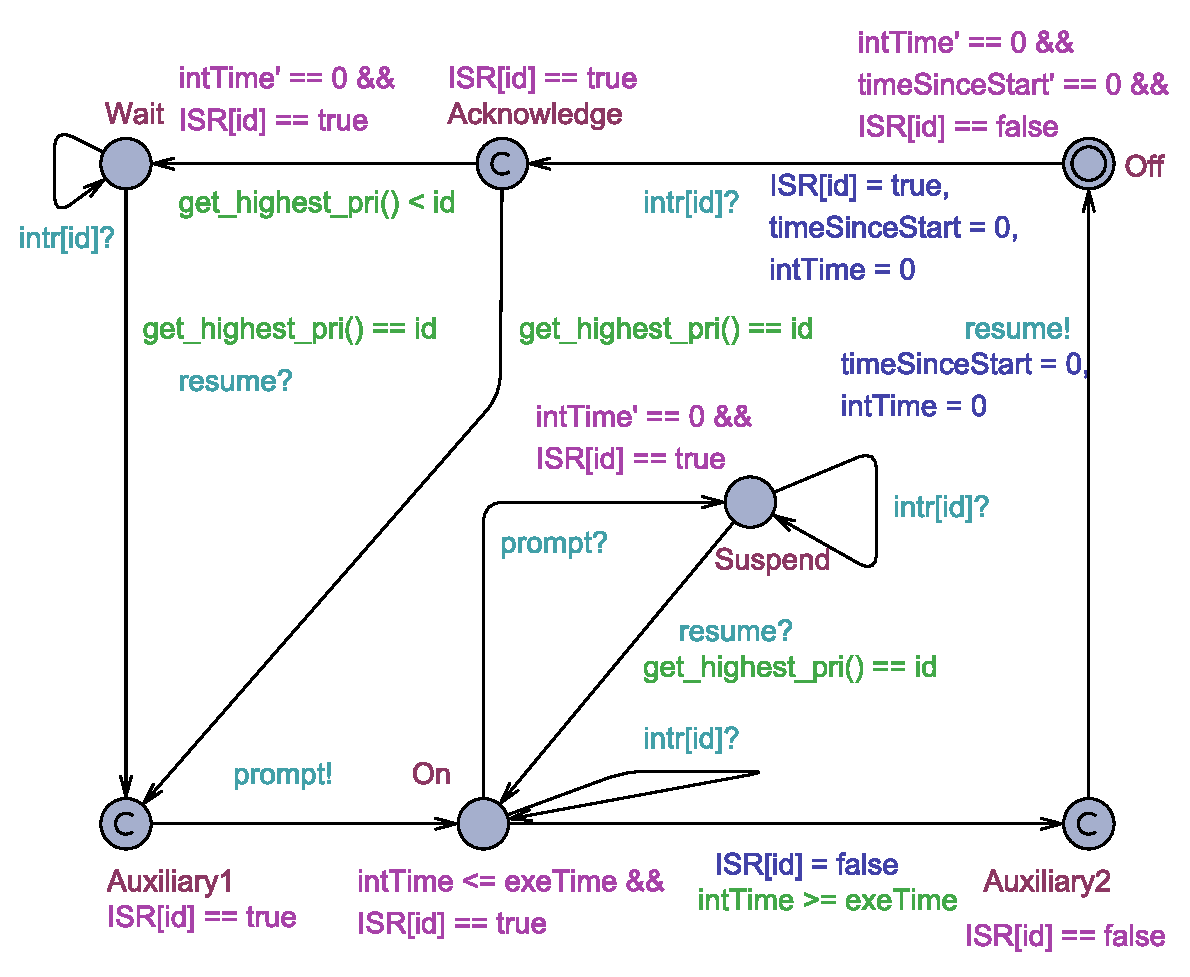
\includegraphics[width=\textwidth]{Interrupt_basic}
	\caption{基本中断的状态机}
	\label{fig:interrupt_basic}
\end{figure}

基本中断的状态机如图~\ref{fig:interrupt_basic} 所示,在这个状态机的状态在Uppaal
中称为位置(Location),以便于整个模型的状态相区分。该模板的内部声明、参数、位置
和变迁的说明分别如表~所示。

\section{带重入的中断模型}
\label{sec:reentrant}

\subsection{重入的硬件实现}
\label{subsec:reentrant_hardware}

\subsection{Uppaal中的重入中断模型}
\label{subsec:reentrant_uppaal}

\section{分段中断模型}
\label{sec:segment}

\subsection{软件的二次实现}
\label{subsec:segment_software}

\subsection{Uppaal中的分段中断模型}
\label{subsec:segment_uppaal}
%%% Local Variables:
%%% mode: latex
%%% TeX-master: t
%%% End:

\chapter{实验}
%%% Local Variables:
%%% mode: latex
%%% TeX-master: t
%%% End:

\chapter{总结}

%%% 其它部分
\backmatter

% 参考文献
\bibliographystyle{thubib}
\bibliography{ref/reference}

% 致谢
%%% Local Variables:
%%% mode: latex
%%% TeX-master: "../main"
%%% End:

\begin{ack}

\end{ack}

%% 附录
%\begin{appendix}
%	\input{data/appendix01}
%\end{appendix}
%
%% 个人简历
\begin{resume}

  \resumeitem{个人简历}

  xxxx 年 xx 月 xx 日出生于 xx 省 xx 县。
  
  xxxx 年 9 月考入 xx 大学 xx 系 xx 专业,xxxx 年 7 月本科毕业并获得 xx 学士学位。
  
  xxxx 年 9 月免试进入 xx 大学 xx 系攻读 xx 学位至今。

  \resumeitem{发表的学术论文} % 发表的和录用的合在一起

  \begin{enumerate}[{[}1{]}]
  \item Yang Y, Ren T L, Zhang L T, et al. Miniature microphone with silicon-
    based ferroelectric thin films. Integrated Ferroelectrics, 2003,
    52:229-235. (SCI 收录, 检索号:758FZ.)
  \item 杨轶, 张宁欣, 任天令, 等. 硅基铁电微声学器件中薄膜残余应力的研究. 中国机
    械工程, 2005, 16(14):1289-1291. (EI 收录, 检索号:0534931 2907.)
  \item 杨轶, 张宁欣, 任天令, 等. 集成铁电器件中的关键工艺研究. 仪器仪表学报,
    2003, 24(S4):192-193. (EI 源刊.)
  \item Yang Y, Ren T L, Zhu Y P, et al. PMUTs for handwriting recognition. In
    press. (已被 Integrated Ferroelectrics 录用. SCI 源刊.)
  \item Wu X M, Yang Y, Cai J, et al. Measurements of ferroelectric MEMS
    microphones. Integrated Ferroelectrics, 2005, 69:417-429. (SCI 收录, 检索号
    :896KM.)
  \item 贾泽, 杨轶, 陈兢, 等. 用于压电和电容微麦克风的体硅腐蚀相关研究. 压电与声
    光, 2006, 28(1):117-119. (EI 收录, 检索号:06129773469.)
  \item 伍晓明, 杨轶, 张宁欣, 等. 基于MEMS技术的集成铁电硅微麦克风. 中国集成电路, 
    2003, 53:59-61.
  \end{enumerate}

  \resumeitem{研究成果} % 有就写,没有就删除
  \begin{enumerate}[{[}1{]}]
  \item 任天令, 杨轶, 朱一平, 等. 硅基铁电微声学传感器畴极化区域控制和电极连接的
    方法: 中国, CN1602118A. (中国专利公开号.)
  \item Ren T L, Yang Y, Zhu Y P, et al. Piezoelectric micro acoustic sensor
    based on ferroelectric materials: USA, No.11/215, 102. (美国发明专利申请号.)
  \end{enumerate}
\end{resume}

\end{document}